\documentclass[11pt]{article}
\usepackage[T1]{fontenc}
\usepackage[utf8]{inputenc}
\usepackage{lmodern}
\usepackage[margin=1in]{geometry}
\usepackage{amsmath,amssymb,amsthm,mathtools,bm}
\usepackage{booktabs,graphicx,microtype}
\usepackage[numbers,sort&compress]{natbib}
\usepackage[colorlinks=true,allcolors=blue]{hyperref}
\usepackage[nameinlink,noabbrev]{cleveref}
\numberwithin{equation}{section}
\newtheorem{theorem}{Theorem}[section]
\newtheorem{proposition}[theorem]{Proposition}
\newtheorem{lemma}[theorem]{Lemma}
\newtheorem{corollary}[theorem]{Corollary}
\theoremstyle{definition}
\newtheorem{definition}[theorem]{Definition}
\newtheorem{assumption}[theorem]{Assumption}
\theoremstyle{remark}
\newtheorem{remark}[theorem]{Remark}
\newcommand{\R}{\mathbb R}
\newcommand{\E}{\mathbb E}
\newcommand{\Prob}{\mathbb P}
\newcommand{\dd}{\,\mathrm d}
\newcommand{\1}{\mathbf 1}
\newcommand{\TV}{\mathrm{TV}}
\newcommand{\Lip}{\mathrm{Lip}}
\newcommand{\pair}[2]{\langle #1,#2\rangle}
\newcommand{\norm}[1]{\left\lVert #1\right\rVert}
\newcommand{\abs}[1]{\left\lvert #1\right\rvert}
\newcommand{\Bc}{B_{\mathrm c}}
\DeclareMathOperator{\supp}{supp}
\DeclareMathOperator{\Var}{Var}
\DeclareMathOperator{\Pois}{Pois}
\title{Sampling-law separation and finite nonlinear corrections\protect\\
in additive coagulation--fragmentation}
\author{}
\date{}
\begin{document}
\maketitle
\begin{abstract}
Additive coagulation with constant per-particle fragmentation can conserve
particle count while the number and mass distributions move toward
opposite size boundaries. We prove fractional-moment inequalities that
quantify this separation, with coefficients that are sharp as uniform
instantaneous constants, for measurable time controls and
parent-dependent expected daughter measures. These coefficients are
Lyapunov bounds, not asymptotic rates: the explicit Golovin--Borel
solution decays several times faster. An auxiliary process with
the normalized number marginals accumulates only a finite upward
log-size correction and undergoes finitely many coagulations almost
surely, even when its expected total number of coagulations is infinite.
For parent-independent daughter fractions, this gives an exact finite
transport cost to a fragmentation reference and transfers compound-Poisson
scaling limits. We bound the last auxiliary coagulation time, prove daughter-law
envelopes that are extremal over all mean-conserving daughter laws, and
obtain exact representations of critical last-event observables in terms
of the unknown law. The open critical exponent reduces to the decay rate
of the deterministic number--mass overlap, and archived simulations
suggest it is near half the coagulation rate. At critical
balance $\sigma=\lambda m$, a physical finite population's normalized
count remains accurate on sublinear time
horizons although mass-distribution error approaches its maximum by
logarithmic times from identical initial data; this is a corollary of
the moment bound and the material ceiling of a finite vessel. Finally, a
Fourier factorization with an exponentially small remainder in time
yields structural fragmentation identification from ideal late-time
distributions on a low-frequency window, at a certified rate whose
asymptotic optimality is not asserted. A separate independent sampling model gives a pointwise
fixed-frequency ratio bound and a sufficient observation-time balance. These results distinguish bulk observability,
auxiliary path asymptotics, and finite-population validity.
\end{abstract}

\section{Introduction}
\label{sec:introduction}

Count, total mass, and mean size do not determine the evolution of a
coagulating and fragmenting population. For the additive kernel
$K(x,y)=\lambda(x+y)$ and constant per-particle fragmentation rate
$\sigma$, mass conservation gives
\[
 N'(t)=(\sigma-\lambda m)N(t).
\]
At the critical balance $\sigma=\lambda m>0$, all three bulk observables
remain fixed. Nevertheless, almost all particles by number become small,
while almost all material is carried by increasingly large particles.
The distinction between selecting a particle and selecting a unit of
material is therefore central to both asymptotic analysis and observation.
Throughout, ``constant fragmentation rate'' means constant per-particle
selection rate; a constant binary fragmentation density can instead
have a size-dependent integrated selection rate.

Population-balance modeling and the recovery of aggregation and breakage
rates from dynamic size distributions have a long history; see
\citet[Chapters 2, 6, and 7]{Ramkrishna2000} for the modeling, inverse,
and stochastic viewpoints, and \citet{Aldous1999,Wattis2006} for
mean-field surveys. Pure additive coagulation is explicitly solvable
\citep{Golovin1963}, has a probabilistic interpretation through
branching structures and the additive coalescent
\citep{AldousPitman1998,DeaconuTanre2000,Bertoin2002}, and a complete
scaling theory \citep{MenonPego2008}. Fractional-moment estimates are
standard tools in the analysis of Smoluchowski equations
\citep{EscobedoMischlerPerthame2002,FournierLaurencot2005,FournierLaurencot2006,EscobedoMischlerRodriguezRicard2005}. Constant count in an evolving population
with aggregation and fragmentation is also established.
\citet{PatilAndrews1998} and \citet{Lage2002} provide constant-count
examples, as explicitly discussed in the introduction of
\citet{McCoyMadras2003}, whose solution allows count to vary.
The results here concern quantitative separation of sampling laws,
its pathwise consequences for the additive model, and the implications
for finite populations and inverse observations.

\subsection{Results and their relation to established ingredients}

The main estimate is a decay inequality for every normalized
fractional moment
$\mathcal A_p=M_p/(N^{1-p}m^p)$, $0<p<1$.
These quantities compare the number law $\eta_t=n_t/N(t)$ with the mass
law $\pi_t=xn_t/m$; at $p=1/2$ they give their Hellinger affinity.
\Cref{thm:affinity} proves
\[
 \mathcal A_p(t)\leq\mathcal A_p(0)
 \exp\!\left[-a_p\int_0^t\lambda(s)m\dd s
             -a_{1-p}\int_0^t\sigma(s)\dd s\right],
 \qquad a_p=1+p-2^p.
\]
The coefficients are sharp as uniform instantaneous coefficients over
the class of solutions and daughter laws, in the explicit sense stated in
the theorem. They are not asymptotic rates: for the Golovin--Borel
solution the exact exponent of $\mathcal A_{1/2}$ is about six times
$a_{1/2}$, and the critical simulations of \cref{sec:finite} show a
similar gap. The pair inequality behind the estimate is a weighted
variant of the subadditivity-defect estimates used in the works cited
above; the contribution is the explicit constant with its equality case
and its uniform use for parent-dependent daughters. At criticality the estimate
proves number concentration at zero, mass escape to infinity, and
nonstationarity without a logarithmic moment assumption. Mass remains
conserved at each finite time.

The same estimate controls the nonlinear contribution to log size.
Probabilistic representations of coagulation equations and changes
between sampling weights are established
\citep{DeaconuTanre2000,DeaconuFournierTanre2002}.
We construct directly an auxiliary number process with marginals
$\eta_t$, including measurable parent-dependent daughters.
Its accumulated upward log increment is finite in mean and almost
surely. A daughter-product martingale then proves that its total
number of coagulation jumps is finite almost surely, although the
mean can be infinite. With selfsimilar daughters, coupling to the
independent fragmentation reference gives an exact extended
Wasserstein cost. Classical compound-Poisson limit theory transfers
to the nonlinear number law, with the daughter log moments needed
for each limit stated separately. Pure-fragmentation logarithmic
asymptotics already appear in
\citet{Bertoin2003,DoumicEscobedo2016}; the finite coagulation
correction supplies the transfer here.

The last auxiliary coagulation gives a stronger path-law comparison.
\Cref{sec:last-event} bounds its tail under arbitrary controls, proves
all-constant-rate daughter-law envelopes by a convexity argument, and
compares them with the number--mass overlap. At criticality the future
hazard is an exponential functional of a compound-Poisson subordinator
\citep{BertoinYor2005}, and the equal-split formula is the Poissonian
exponential functional of \citet{BertoinBianeYor2004}. We derive exact
representations of last-event observables and a density in terms of
the unknown law, together with upper and lower calendar-time tail
bounds. The exponent between these bounds is not determined; the
envelopes reduce it to the decay rate of the deterministic overlap, and
the archived simulations suggest the value $b/2$ of the pure-coagulation
benchmark. The Golovin--Borel solution \citep{Golovin1963}, recorded by
\citet{Bertoin2009}, provides that benchmark. These established
formulas are used with explicit attribution.

A finite physical population must obey a total-material ceiling that
the continuum equation does not share. Differences between finite
stochastic coagulation--fragmentation systems and mean-field predictions
are already documented, for example by
\citet{DOrsognaLeiChou2015} in a finite-cluster assembly model.
For the present critical additive model, \cref{sec:finite} records an
explicit distinction in growing time: starting from exactly the same
empirical initial measure, mass cumulative distributions have nearly
maximal discrepancy at least by times proportional to the logarithm of
population scale, while normalized count is uniformly accurate on every
sublinear horizon. The discrepancy statement is a corollary of the
moment bound and the material ceiling of a finite vessel; only the count
statement uses the particle dynamics. Nine reproducible particle runs
illustrate separation diagnostics and the gap between certified and
observed decay rates. They do not compute a continuum comparison.

Finally, the integrable nonlinear log correction gives a Fourier
factorization whose remainder is exponentially small in time, at the
certified rate $\kappa(b+\sigma)$. Local late-time quotients on a
low-frequency window identify the fragmentation exponent and, by
one-sided transform uniqueness, the expected daughter fraction measure.
The second step is analytic continuation from a short interval and is
severely ill-posed. This sits within established
inverse population-balance work: \citet{DoumicEscobedoTournus2018}
uses asymptotic fragmentation profiles,
\citet{DoumicEscobedoTournus2024} uses short-time distributions,
and \citet{MirzaevByrneBortz2016} estimates daughter distributions in
an aggregation--fragmentation model. Two-time quotient cancellation
and distinguished logarithms have a direct precedent in
\citet[Section 2.2]{Garnier2024}. The contribution of
\cref{sec:fourier} is the proved nonlinear remainder and its
identification consequence for additive coagulation. The statistical
application is a pointwise bound under independent sampling,
with no claim of stable recovery of a whole daughter measure or
of statistical optimality.

\subsection{Scope, assumptions, and organization}

Three different probabilistic objects occur. The auxiliary process
represents one-time continuum number laws; its jumps are not a physical
material genealogy. The finite particle system describes an actual
mass-conserving vessel with interacting particles. The empirical Fourier
sampling bound assumes independent draws from deterministic continuum
marginals. No independence or approximation between these objects is
implicit in the results.

\Cref{tab:assumptions} records the main changes of assumptions.
All deterministic estimates are conditional on the mass-conserving
weak-solution framework in \cref{sec:model}.
\Cref{thm:existence,app:existence} prove existence and uniqueness with
finite initial second moment, while most asymptotic estimates use only
finite number and mass once a solution is supplied.
A finite second size moment does not imply an integrable negative
log size. No logarithmic moment is silently inherited from that
existence theorem.

\begin{table}[htbp]
\centering\small
\begin{tabular}{p{0.29\textwidth}p{0.64\textwidth}}
\toprule
Results & Additional scope or assumptions \\
\midrule
Sampling separation and finite auxiliary correction
& Locally integrable time controls; measurable parent-dependent expected
  daughters with count two and conserved mean mass. \\
Transport and logarithmic limits
& Parent-independent fractions for the independent reference; fixed rates
  and fraction law for stationary increments; daughter log moments as stated. \\
Daughter envelopes and critical representations
& Constant rates; critical formulas require $\sigma=\lambda m$;
  equal splitting only for the formulas labeled as such. \\
Finite-population comparison
& Critical rates and eventwise complementary positive binary splits;
  continuum and particles start from the identical empirical measure. \\
Fourier identification and sampling
& Constant $\lambda>0$, $\sigma\geq0$, and fixed parent-independent $B$;
  exact distributions for identification, independent samples for the sampling bound. \\
\bottomrule
\end{tabular}
\caption{Assumption roadmap. Individual statements specify all moment,
observation, and solution hypotheses.}
\label{tab:assumptions}
\end{table}

\Cref{sec:boundaries} adds the complete fixed-mass count-neutral
classification, rigidity from one further moment, and the failure of
fractional-moment monotonicity beyond the additive kernel. These results
clarify which conclusions depend on the additive structure.
Elementary finite-grid preparation and initial-rate algebra, including
dilution and source ambiguities, are collected in a supplementary note
distributed with the numerical supplement.
The appendices contain forward well-posedness, product error
certification, finite-count formulas, and unbounded-test justifications.
\Cref{sec:discussion} separates the proved conclusions from the remaining
asymptotic and statistical questions.

\section{Model, solution framework, and sampling laws}
\label{sec:model}

The size variable $x\in E:=(0,\infty)$ is proportional to particle mass.
We fix its reference unit throughout, so that logarithms of size and sums such
as $1+x$ below are dimensionless. The finite nonnegative measure $n_t$ describes
particle number per unit volume. For $p\geq0$, write
\begin{equation}
 M_p(t)=\int_E x^p n_t(\dd x),\qquad N(t)=M_0(t),\qquad m=M_1(0).
 \label{eq:moments}
\end{equation}
We assume $0<N_0:=N(0)<\infty$ and $0<m<\infty$.

\begin{assumption}[Rates and daughters]\label{ass:rates}
The functions $\lambda,\sigma:[0,\infty)\to[0,\infty)$ are measurable and
locally integrable. Coagulation has the additive kernel
$K_t(x,y)=\lambda(t)(x+y)$. Fragmentation has per-particle selection rate
$\sigma(t)$. Its expected daughter measure is a measurable kernel
$(t,x)\mapsto b_{t,x}$ on $E$, satisfying
\begin{equation}
 b_{t,x}(E\setminus(0,x))=0,\qquad
 \int_E b_{t,x}(\dd z)=2,\qquad
 \int_E z\,b_{t,x}(\dd z)=x.
 \label{eq:daughters}
\end{equation}
These conditions hold for every $(t,x)$; the values of the model at a common
null set of times may be chosen arbitrarily subject to these conditions.
\end{assumption}

Only the expected daughter count and mass enter the deterministic equation.
An actual binary split has expected measure
$\E[\delta_{Vx}+\delta_{(1-V)x}]$ for a random $V\in(0,1)$.
Conditions \eqref{eq:daughters} allow a larger class of expected measures:
they do not require symmetry about $x/2$, which an eventwise complementary
binary split would impose. Results about a finite system of particles will
explicitly require eventwise binary mass conservation. Unless stated otherwise,
the deterministic results use only \eqref{eq:daughters}.

Write $\pair{f}{\mu}=\int_E f\dd\mu$ whenever this integral is defined.
For a Borel test $f$, define
\begin{equation}
 \Delta f(x,y)=f(x+y)-f(x)-f(y),\qquad
 \mathcal F_t f(x)=\int_E f(z)b_{t,x}(\dd z)-f(x).
 \label{eq:increments}
\end{equation}
The weak population balance is
\begin{align}
 \pair{f}{n_t}-\pair{f}{n_0}
 &=\frac12\int_0^t\lambda(s)\iint_{E^2}(x+y)\Delta f(x,y)
                  n_s(\dd x)n_s(\dd y)\dd s\notag\\
 &\quad+\int_0^t\sigma(s)\int_E\mathcal F_s f(x)n_s(\dd x)\dd s.
 \label{eq:weak}
\end{align}
The factor $1/2$ counts each unordered coagulation pair once.

\begin{definition}[Mass-conserving solution]\label{def:solution}
A solution is a curve of nonnegative finite measures $n_t$ on $E$ such that
$t\mapsto n_t(A)$ is measurable for each Borel set $A\subset E$,
with $\sup_{s\leq T}N(s)<\infty$ for every $T<\infty$, constant first moment
$M_1(t)=m$, and \eqref{eq:weak} for every bounded Borel $f$ and every $t\geq0$.
\end{definition}

All terms in this definition are absolutely integrable on bounded time
intervals: their absolute values are bounded using
$\iint(x+y)n_s(\dd x)n_s(\dd y)=2mN(s)$ and
$|\mathcal F_s f|\leq3\norm{f}_\infty$.
In particular the solution is continuous in total variation.
For a signed measure $\mu$, write
\begin{equation}
 \norm{\mu}_w=\int_E(1+x)|\mu|(\dd x),\qquad
 \norm{\mu}_{\mathrm{var}}=|\mu|(E).
 \label{eq:variation}
\end{equation}
For probability measures the distance
$\norm{\mu-\nu}_{\TV}:=\sup_A|\mu(A)-\nu(A)|$
equals $\tfrac12\norm{\mu-\nu}_{\mathrm{var}}$.

\begin{theorem}[A well-posed solution class]\label{thm:existence}
Under \cref{ass:rates}, suppose additionally that $M_2(0)<\infty$.
There is a unique mass-conserving solution with locally bounded second
moment. It is continuous in the weighted-variation norm $\norm{\cdot}_w$
and satisfies
\begin{equation}
 M_2(t)\leq M_2(0)\exp\left(2m\int_0^t\lambda(s)\dd s\right).
 \label{eq:M2bound}
\end{equation}
No continuity of the daughter kernel in the parent variable is required.
\end{theorem}

A self-contained proof appears in \cref{app:existence}. It uses a
weighted-variation stability estimate and approximations that converge in
that norm. This avoids passing a merely measurable parent-dependent kernel
through a narrow limit. The proof also avoids treating weak integrals of
moving atomic measures as Bochner integrals. We use the second moment as a
sufficient condition for this construction, not as a necessary condition for
the population balance or the results below. In the time-independent
selfsimilar setting, weaker initial-moment assumptions are available for
fixed relative-fragment laws satisfying the dislocation hypotheses of
\citet{Cepeda2014}. That work treats homogeneous-like coagulation and
multiple fragmentation using a Wasserstein-type distance. The finite first
moment is the relevant homogeneity moment for the additive kernel. Neither
that result nor the proof here is a claim of novelty for existence methods.

The estimates that follow require only \cref{def:solution}, unless a theorem
explicitly adds moment assumptions. Thus they also apply to any separately
constructed finite-count, finite-mass solution outside \cref{thm:existence}.
This distinction is useful for logarithmic observables: neither a finite
second size moment nor finite count and mass implies a finite negative
logarithmic moment.

Set
\begin{equation}
 b(t)=m\lambda(t),\qquad
 \Bc(t)=\int_0^t b(s)\dd s,\qquad
 F(t)=\int_0^t\sigma(s)\dd s,\qquad C(t)=\Bc(t)+F(t).
 \label{eq:clocks}
\end{equation}
Here $b(t)$ is a scalar rate; the two-index symbol $b_{t,x}$ always denotes
the daughter measure. Testing \eqref{eq:weak} with $f=1$ shows that $N$ is
locally absolutely continuous, with
\begin{equation}
 N'(t)=(\sigma(t)-b(t))N(t)\quad\text{for almost every }t,\qquad
 N(t)=N_0e^{F(t)-\Bc(t)}\quad(t\geq0).
 \label{eq:count}
\end{equation}
In particular $N(t)>0$ at each finite time. The number and mass sampling laws
are respectively
\begin{equation}
 \eta_t(\dd x)=\frac{n_t(\dd x)}{N(t)},\qquad
 \pi_t(\dd x)=\frac{x\,n_t(\dd x)}{m},\qquad
 \frac{\dd\pi_t}{\dd\eta_t}(x)=\frac{N(t)x}{m}.
 \label{eq:sampling}
\end{equation}
The first law samples particles uniformly by number; the second samples a
uniform unit of material and records the size of its containing particle.
Their distinction is central even when their underlying population is the
same. Probabilistic representations of mass sampling in pure coagulation
are established; see, for example, \citet{DeaconuFournierTanre2002}.

For $0<p<1$, define the normalized fractional moment
\begin{equation}
 \mathcal A_p(t)=\frac{M_p(t)}{N(t)^{1-p}m^p}
 =\int_E\left(\frac{\dd\pi_t}{\dd\eta_t}\right)^p\dd\eta_t.
 \label{eq:affinity}
\end{equation}
H\"older's inequality gives $0<\mathcal A_p\leq1$.
At $p=1/2$ it is the Hellinger affinity of the two sampling laws.
No density of $n_t$ with respect to Lebesgue measure is assumed anywhere in
these definitions.

\section{Fractional-moment decay and sampling-law separation}
\label{sec:fractional}

\subsection{The pair inequality and admissible moment tests}

\begin{lemma}[Sharp fractional pair inequality]\label{lem:pair}
For $x,y>0$ and $0<p<1$,
\begin{equation}
 (x+y)\bigl[x^p+y^p-(x+y)^p\bigr]
 \geq(2-2^p)(xy^p+yx^p).
 \label{eq:pair}
\end{equation}
Equality holds exactly when $x=y$.
\end{lemma}

\begin{proof}
Put $u=x/(x+y)$, $v=1-u$, and $A=2^p-1\in(0,1)$.
After division by $(x+y)^{p+1}$, \eqref{eq:pair} is equivalent to
$g(u)\geq1$, where
\[
 g(u)=A(u^p+v^p)+(1-A)(u^{p+1}+v^{p+1}).
\]
By symmetry it suffices to consider $0<u<1/2$. The continuous endpoint
values are $g(0)=g(1/2)=1$, whereas $g'(0+)=+\infty$ and $g'(1/2)=0$.
The sign of $g''(u)$ is the sign of
\[
 (1-A)(p+1)-A(1-p)R(u),\qquad
 R(u)=\frac{u^{p-2}+v^{p-2}}{u^{p-1}+v^{p-1}}
     =\frac{u^{2-p}+v^{2-p}}{uv(u^{1-p}+v^{1-p})}.
\]
On $(0,1/2)$ the numerator in the final expression strictly decreases,
and each positive factor in its denominator strictly increases. Hence $R$
strictly decreases and $g''$ changes sign at most once, from negative to
positive. This change must occur. Since $R(u)\to+\infty$ as
$u\downarrow0$, $g''<0$ near $0$; equivalently, $g'(0+)=+\infty$ is
incompatible with $g'$ increasing on $(0,1/2)$ to the value $g'(1/2)=0$.
Nor can $g''$ remain negative: then $g'$ would decrease to zero while
remaining positive, contradicting the equal endpoint values of $g$.
On the final interval where $g''>0$, the derivative approaches zero from
below. On the initial interval it therefore crosses zero exactly once.
Thus $g$ first increases and then decreases to its endpoint value $1$,
and $g(u)>1$ in $(0,1/2)$. This proves the inequality and its equality case.
\end{proof}

Estimates of the subadditivity defect $x^p+y^p-(x+y)^p$ are standard
tools in the fractional-moment analysis of Smoluchowski equations; see
\citet{EscobedoMischlerPerthame2002},
\citet{FournierLaurencot2005,FournierLaurencot2006}, and
\citet{EscobedoMischlerRodriguezRicard2005}. Inequality \eqref{eq:pair}
is a weighted variant of these estimates, with the additive weight $x+y$
built in. The contribution here is the explicit constant $2-2^p$ with its
equality case, and its use below as a uniform coefficient for
parent-dependent daughters.

\begin{lemma}[Fractional moment balance]\label{lem:moment-balance}
For every solution in \cref{def:solution} and every $0<p<1$, $M_p$ is
locally absolutely continuous. Its weak balance is \eqref{eq:weak} with
$f(x)=x^p$, with absolutely integrable right-hand side on finite intervals.
\end{lemma}

\begin{proof}
H\"older's inequality gives $M_p(t)\leq N(t)^{1-p}m^p$.
Use the bounded Borel tests $f_R(x)=\min(x^p,R)$.
They are increasing, concave, and subadditive, with $f_R(0)=0$.
Consequently
\[
 0\leq f_R(x)+f_R(y)-f_R(x+y)\leq\min(x^p,y^p).
\]
After multiplication by $x+y$ this is bounded by $xy^p+yx^p$,
whose integral against $n_t\otimes n_t$ is $2mM_p(t)$.
For daughters, $f_R(z)/z$ is nonincreasing in $z$; since $z<x$ and
daughter mass is conserved,
\[
 0\leq\int_E f_R(z)b_{t,x}(\dd z)-f_R(x)
 \leq\int_E z^p b_{t,x}(\dd z)\leq2^{1-p}x^p.
\]
The last inequality is Jensen's inequality for the probability
$b_{t,x}/2$, whose mean is $x/2$. These bounds are uniform in $R$ and
integrable in time after multiplication by the locally integrable rates.
Monotone convergence on the left and dominated convergence on the right
of \eqref{eq:weak} yield the asserted identity. Its integrable right-hand
side also proves local absolute continuity.
\end{proof}

\subsection{A uniform estimate for controlled rates}

Write
\begin{equation}
 a_p=1+p-2^p>0\quad(0<p<1),\qquad
 \kappa=3-2\sqrt2=2a_{1/2}>0.
 \label{eq:constants}
\end{equation}
Positivity of $a_p$ follows from strict convexity of $2^p$ and its chord
between $p=0$ and $p=1$.

\begin{theorem}[Separation of the sampling laws]\label{thm:affinity}
Under \cref{ass:rates,def:solution}, for every $0<p<1$,
\begin{align}
 M_p'(t)&\leq
 \bigl[-b(t)(2-2^p)+\sigma(t)(2^{1-p}-1)\bigr]M_p(t)
 \quad\text{for almost every }t,\label{eq:raw-moment}\\
 \mathcal A_p(t)&\leq\mathcal A_p(0)
        e^{-a_p\Bc(t)-a_{1-p}F(t)}.\label{eq:affinity-decay}
\end{align}
In particular, writing $H(t)=M_{1/2}(t)$,
\begin{equation}
 \frac{H(t)^2}{N(t)}\leq\frac{H(0)^2}{N_0}e^{-\kappa C(t)}.
 \label{eq:half-decay}
\end{equation}
The coefficients are instantaneously sharp in the following sense: if
constants $c_1,c_2$ satisfy
$\mathcal A_p(t)\leq\mathcal A_p(0)e^{-c_1\Bc(t)-c_2F(t)}$ for all
$t\geq0$, all solutions of \cref{thm:existence}, and all daughter kernels
satisfying \eqref{eq:daughters}, then $c_1\leq a_p$ and $c_2\leq a_{1-p}$.
\end{theorem}

\begin{proof}
By \cref{lem:pair}, the coagulation term in the fractional moment balance
is at most $-\lambda(t)(2-2^p)mM_p(t)$. Jensen's inequality in the proof of
\cref{lem:moment-balance} bounds the fragmentation contribution by
$\sigma(t)(2^{1-p}-1)M_p(t)$. This proves \eqref{eq:raw-moment}.
Differentiate the number normalization using \eqref{eq:count}.
Its contribution is $-(1-p)(\sigma-b)$, and the resulting coefficients
are $-a_p b-a_{1-p}\sigma$. An integrating factor proves
\eqref{eq:affinity-decay} without dividing by $M_p$.
Taking $p=1/2$ and squaring gives \eqref{eq:half-decay}.

For the sharpness statement take constant rates, initial data
$n_0=N_0\delta_{x_0}$, and equal daughters $b_x=2\delta_{x/2}$, so that
$\mathcal A_p(0)=1$. For $f(x)=x^p$, weighted-variation continuity from
\cref{thm:existence}, the bound
$(x+y)|\Delta f(x,y)|\leq xy^p+yx^p\leq2(1+x)(1+y)$,
and the equal-split identity $\mathcal F f(x)=(2^{1-p}-1)x^p$ make the
moment-balance integrand continuous at zero. Thus $M_p$ has a right
derivative at zero, equal to the value of the vector field at $n_0$.
There both the pair inequality and Jensen's inequality are equalities, so
$M_p'(0+)=[-b(2-2^p)+\sigma(2^{1-p}-1)]M_p(0)$, and by \eqref{eq:count}
$\mathcal A_p'(0+)=-a_pb-a_{1-p}\sigma$. Now let $c_1,c_2$ satisfy the
stated bound. With $\sigma=0$ and $\lambda>0$ the bound gives
$\mathcal A_p(t)\leq1-c_1bt+o(t)$ as $t\downarrow0$, while
$\mathcal A_p(t)=1-a_pbt+o(t)$; hence $c_1\leq a_p$. With $\lambda=0$ and
$\sigma>0$ the same comparison gives $c_2\leq a_{1-p}$.

For equal splitting the identity $\int z^pb_x(\dd z)=2^{1-p}x^p$ holds for
every parent size $x$, not only at a monodisperse state. Hence with
$\lambda=0$, \cref{lem:moment-balance} gives
$M_p(t)=M_p(0)e^{(2^{1-p}-1)F(t)}$ and, by \eqref{eq:count},
$\mathcal A_p(t)=\mathcal A_p(0)e^{-a_{1-p}F(t)}$ for every initial measure
and every $t\geq0$. The fragmentation coefficient is then exact for all
times, not only instantaneously.
\end{proof}

\begin{remark}[What the estimate compares]\label{rem:relative}
If $C(t)\to\infty$, the sampling laws separate in total variation, because
\begin{equation}
 1-\norm{\eta_t-\pi_t}_{\TV}
 =\int_E\min\left(1,\frac{N(t)x}{m}\right)\eta_t(\dd x)
 \leq\mathcal A_p(t)\longrightarrow0.
 \label{eq:overlap-affinity}
\end{equation}
This concerns relative number and mass sampling. Outside the critical
case below it does not imply that raw mass moves to arbitrarily large
sizes.

Instantaneous sharpness does not identify the long-time exponent for a
prescribed daughter law or initial distribution, and the gap can be
large. For pure additive coagulation ($\sigma=0$, constant $\lambda$,
unit monodisperse initial data with $N_0=m=1$, so that $b=\lambda$) the
explicit solution of \citet{Golovin1963}, recorded in \citet{Bertoin2009},
has $N(t)=e^{-bt}$ and number law $\eta_t$ equal to the Borel law with
parameter $\mu_t=1-e^{-bt}$, that is
$\eta_t(\{k\})=e^{-\mu_tk}(\mu_tk)^{k-1}/k!$; for its probabilistic
interpretation see \citet{DeaconuTanre2000,Bertoin2002}, and for the
scaling theory of this kernel see \citet{MenonPego2008}. As $t\to\infty$
the number law converges to the Borel law with parameter one, whose tail
is of order $k^{-3/2}$. Consequently $M_p/N$ stays bounded for $p<1/2$ and
grows like $e^{(2p-1)bt}$ for $p>1/2$, and $\mathcal A_p=(M_p/N)N^p$
decays at the exact exponential rate $\min(p,1-p)\,b$, in the sense that
$-t^{-1}\log\mathcal A_p(t)\to\min(p,1-p)\,b$. For $p=1/2$ this is about
six times the coefficient $a_{1/2}\approx0.086$ in
\eqref{eq:affinity-decay}. The critical equal-split particle simulations
of \cref{sec:finite} show a gap of the same kind: for the largest
population the fitted late-time decay rate of $\mathcal A_{1/2}$ is about
$0.45b$, against the guaranteed $\kappa b\approx0.17b$. The estimate is
therefore a uniform Lyapunov bound, valid for every admissible daughter
law and initial measure, not an asymptotic rate.
\end{remark}

\subsection{Criticality: constant count and motion toward both boundaries}

Suppose now that $\lambda>0$ is constant and $\sigma=b$, so that both
rates are constant.
The daughter measure may still depend measurably on time and parent size.
Count remains exactly $N_0$. Set
\begin{equation}
 \kappa_p=3-2^p-2^{1-p}=a_p+a_{1-p}>0.
 \label{eq:kappap}
\end{equation}

\begin{corollary}[Two-boundary separation]\label{cor:critical}
At criticality, for every $0<p<1$,
\begin{equation}
 M_p(t)\leq M_p(0)e^{-b\kappa_p t}.
 \label{eq:critical-moment}
\end{equation}
For each fixed $p$ the coefficient is instantaneously sharp in the
sense of \cref{thm:affinity}: if $M_p(t)\leq M_p(0)e^{-cbt}$ for all
$t\geq0$, all critical solutions of \cref{thm:existence}, and all daughter
kernels satisfying \eqref{eq:daughters}, then $c\leq\kappa_p$. Among these
coefficients the unique maximum is $\kappa_{1/2}=\kappa$.
For every $\varepsilon,R>0$,
\begin{align}
 n_t([\varepsilon,\infty))
   &\leq\varepsilon^{-p}M_p(0)e^{-b\kappa_p t},\label{eq:number-window}\\
 \int_{(0,R]}x\,n_t(\dd x)
   &\leq R^{1-p}M_p(0)e^{-b\kappa_p t}.\label{eq:mass-window}
\end{align}
Viewed as measures on $[0,\infty)$, $n_t$ converges weakly to
$N_0\delta_0$. On the compactified space $[0,\infty]$, $\pi_t$ converges
weakly to $\delta_\infty$. No nonzero stationary solution with finite count
and positive finite mass exists.
\end{corollary}

\begin{proof}
Equation \eqref{eq:critical-moment} follows from \eqref{eq:raw-moment};
its sharpness follows from the monodisperse equal-split example in the
proof of \cref{thm:affinity}, where $M_p'(0+)=-b\kappa_pM_p(0)$, so
$M_p(t)=M_p(0)(1-b\kappa_pt+o(t))$ and $c\leq\kappa_p$.
The strict convexity and symmetry of $2^p+2^{1-p}$ give its unique minimum
$2\sqrt2$ at $p=1/2$, and its value is strictly below the common endpoint
value $3$ in $(0,1)$.
On $[\varepsilon,\infty)$, $x^p\geq\varepsilon^p$; on $(0,R]$,
$x\leq R^{1-p}x^p$. These prove the window bounds.
For a bounded continuous function on $[0,\infty)$, its oscillation near
zero is small and the number outside that neighborhood tends to zero.
This proves the first weak limit. A continuous function on
$[0,\infty]$ is uniformly close to its value at infinity outside a
sufficiently large bounded interval; \eqref{eq:mass-window} proves the
second limit. A stationary measure would have $M_p>0$ constant in time,
contradicting \eqref{eq:critical-moment}.
\end{proof}

Both limits are long-time statements. All material mass is conserved at
every finite time. The particles that become rare in number carry most
of the material. There is no assertion of finite-time shattering or
gelation. On a fixed bounded size interval with an upper cutoff $R$,
positive mass $m$ forces $M_p\geq m/R^{1-p}$; hence a discretization that
confines all mass there cannot satisfy \eqref{eq:critical-moment}
indefinitely.

\begin{corollary}[Exponentially moving observation windows]\label{cor:moving}
For $\varepsilon_0,R_0>0$ and $0<v<b\log2$, both
\begin{equation}
 n_t([\varepsilon_0e^{-vt},\infty))\longrightarrow0,\qquad
 \int_{(0,R_0e^{vt}]}x\,n_t(\dd x)\longrightarrow0
 \label{eq:moving}
\end{equation}
at exponential rates.
\end{corollary}

\begin{proof}
The two respective bounds, for arbitrary $p\in(0,1)$, are
\[
 \varepsilon_0^{-p}M_p(0)e^{-[b\kappa_p-pv]t},\qquad
 R_0^{1-p}M_p(0)e^{-[b\kappa_p-(1-p)v]t}.
\]
Since $\kappa_p/p\to\log2$ as $p\downarrow0$ and
$\kappa_p/(1-p)\to\log2$ as $p\uparrow1$, a suitable exponent exists
for each bound. They generally use different exponents $p$.
Since $\kappa_p$ is concave with $\kappa_0=0$, the quotient $\kappa_p/p$
decreases in $p$, so $\sup_{0<p<1}\kappa_p/p=\log2$; by the symmetry
$\kappa_p=\kappa_{1-p}$ the same holds for $\kappa_p/(1-p)$. Thus
$v<b\log2$ is exactly the range this argument reaches.
\end{proof}

These guaranteed velocities do not give a matching asymptotic front
speed. The endpoint $v=b\log2$ is not included.

\subsection{A nonstationarity criterion under rate perturbations}

\begin{proposition}[A sufficient open rate condition]\label{prop:robust}
Consider a jointly measurable symmetric kernel $(t,x,y)\mapsto K_t(x,y)$
and jointly measurable selection rate $(t,x)\mapsto S_t(x)$ satisfying
\begin{equation}
 a(x+y)\leq K_t(x,y)\leq A(x+y),\qquad
 0\leq S_t(x)\leq s_*,\qquad 0<a\leq A<\infty,
 \label{eq:robust-assumptions}
\end{equation}
with daughters as in \cref{ass:rates}. Use \cref{def:solution} with
$\lambda(s)(x+y)$ replaced by $K_s(x,y)$ in the coagulation term of
\eqref{eq:weak}, and $\sigma(s)\mathcal F_s f(x)$ replaced by
$S_s(x)\mathcal F_s f(x)$ in the fragmentation term. In particular, the
balance holds for every bounded Borel test, count is locally bounded,
and mass is conserved. For every such solution of mass $m$ and every
$0<p<1$,
\begin{equation}
 M_p(t)\leq M_p(0)e^{-\gamma_p t},\qquad
 \gamma_p=(2^{1-p}-1)(am\,2^p-s_*).
 \label{eq:robust}
\end{equation}
If $s_*<2am$, no stationary measure of mass $m$ has finite positive
particle count.
\end{proposition}

\begin{proof}
The count balance gives $N(t)\leq N_0e^{s_*t}$. The upper bounds in
\eqref{eq:robust-assumptions} and the proof of
\cref{lem:moment-balance} justify the fractional test. Its coagulation
contribution is at most $-am(2-2^p)M_p$ by the lower kernel bound,
and fragmentation contributes at most $s_*(2^{1-p}-1)M_p$.
Their difference equals $-\gamma_pM_p$ because
$2-2^p=2^p(2^{1-p}-1)$.
If $s_*<2am$, choose $p<1$ close enough to one that $am2^p>s_*$.
A stationary measure would then have a strictly positive moment that
decays exponentially, a contradiction.
\end{proof}

The threshold here is sufficient. We make no claim of its optimality or
of existence of stationary solutions above it. Count need not be constant
under \eqref{eq:robust-assumptions}.

\section{An auxiliary number process and its finite coagulation correction}
\label{sec:auxiliary}

Fix a solution in \cref{def:solution}. In this section the rates and
daughter kernel retain the full generality of \cref{ass:rates}.
The construction uses the deterministic curve $n_t$ as its environment.
Its one-time laws are the number sampling laws $\eta_t$, but its paths
are not physical mass tags or chronological particle lineages.

\subsection{Construction and identification of the marginals}

\begin{theorem}[Number-weighted jump representation]\label{thm:number-process}
There is a nonexplosive time-inhomogeneous Markov jump process $X_t$
on $E$, with initial law $\eta_0$, whose law at every $t$ is $\eta_t$.
Its generator, meaning its jump kernel acting on bounded Borel
functions $f$, is
\begin{align}
 \mathcal L_t f(x)
 &=\sigma(t)\int_E[f(z)-f(x)]b_{t,x}(\dd z)\notag\\
 &\quad+\lambda(t)N(t)x\int_E[f(x+y)-f(x)]\eta_t(\dd y).
 \label{eq:number-generator}
\end{align}
Thus fragmentation occurs at rate $2\sigma(t)$ and selects a daughter
with law $b_{t,x}/2$. Coagulation occurs at rate $\lambda(t)N(t)x$
and adds a fresh sample from the prescribed law $\eta_t$.
The fragmentation term has a direct interpretation: a fragmentation
event replaces the tagged particle by one of its two daughters chosen
uniformly, which has law $b_{t,x}/2$; number weighting counts both
daughters, so the number-weighted process sees this daughter law at
twice the selection rate $\sigma(t)$.
\end{theorem}

\begin{proof}
Symmetry rewrites the coagulation term of \eqref{eq:weak} as
\[
 \lambda(t)\iint x[f(x+y)-f(x)-f(y)]n_t(\dd x)n_t(\dd y).
\]
For each bounded Borel $f$, divide its scalar, absolutely continuous
balance by $N(t)$ and use \eqref{eq:count}. The result is
\begin{equation}
 \pair{f}{\eta_t}-\pair{f}{\eta_0}
 =\int_0^t\pair{\mathcal L_s f}{\eta_s}\dd s.
 \label{eq:number-forward}
\end{equation}
All these integrals are finite on bounded time intervals.

For the construction use two independent Poisson random measures,
independent also of $X_0$. The fragmentation driver has intensity
$2\sigma(t)\dd t\dd u$, $0<u<1$; the quantile map
$(t,x,u)\mapsto\inf\{z:b_{t,x}((0,z])/2\geq u\}$ chooses its
daughter using $u$. This map is jointly measurable: the set where
it is at most $z$ equals $\{(t,x,u):b_{t,x}((0,z])/2\geq u\}$,
by right-continuity in $z$ of the distribution function, and
$(t,x,z)\mapsto b_{t,x}((0,z])$ is measurable because $b$ is a
measurable kernel. The coagulation driver has
intensity $\dd t\dd v\dd u$, $v>0$, $0<u<1$; retain a point when
$v\leq\lambda(t)N(t)X_{t-}$ and use the quantile map of $\eta_t$,
jointly measurable in $(t,u)$ for the same reason, to choose its
added size. Let $(\mathfrak F_t)_{t\geq0}$ be the filtration
generated by $X_0$ and the two driving Poisson random measures,
augmented with the $\Prob$-null sets; it satisfies the usual
conditions. Because the two drivers are independent of each other
and of $X_0$, each driver keeps its deterministic compensator in
this joint filtration. All stopping times, compensators, and local
martingales in this section refer to $(\mathfrak F_t)$.
Recursive construction
up to successive jumps gives the minimal process, initially defined
up to a possible explosion time. Its jump kernel $Q_t(x,\dd z)$ is
the sum of the two positive kernels in \eqref{eq:number-generator},
and its total rate is
\begin{equation}
 q_t(x)=2\sigma(t)+\lambda(t)N(t)x.
 \label{eq:number-total-rate}
\end{equation}
These rates are bounded by an integrable time function on every
bounded size set and finite time interval.

Here is a first-moment nonexplosion argument. Daughter mass conservation
and $\pair{x}{\eta_t}=m/N(t)$ give, for $V(x)=x$,
\begin{equation}
 \mathcal L_t V(x)=(b(t)-\sigma(t))x\leq b(t)x.
 \label{eq:number-lyapunov}
\end{equation}
The generator was defined on bounded functions; its application to
the unbounded $V$ is justified by the stopping that follows, which
keeps every term of the Dynkin formula finite.
Stop at the $k$th jump $\tau_k$ and at $\tau_R$, the first time
the state exceeds $R$.
Before these stops rates are integrably bounded. An upward jump can
overshoot $R$, but its mark has finite conditional mean $m/N(t)$;
the expected positive and negative increments in the stopped Dynkin
formula are therefore finite. Gronwall's inequality gives
$\E X_{t\wedge\tau_k\wedge\tau_R}\leq\E X_0e^{\Bc(t)}$.
For fixed $k$, only finitely many finite states are visited, so the
size stopping can be removed as $R\to\infty$. Fatou's lemma yields
\begin{equation}
 \E X_{t\wedge\tau_k}\leq\frac m{N_0}e^{\Bc(t)}.
 \label{eq:stopped-first-moment}
\end{equation}
The jump-count compensator is the time integral of the conditional
jump rate; after integrable stopping, its expectation equals the
expected jump count. The compensator of the stopped total jump count has
expectation at most
\begin{equation}
 L_T:=2F(T)+\frac m{N_0}
       \int_0^T\lambda(s)N(s)e^{\Bc(s)}\dd s<\infty.
 \label{eq:stopped-jump-bound}
\end{equation}
With the size stop in place all rates are integrably bounded, so
the compensator identity is exact; as $R\to\infty$ the stopped
counts and their compensators increase to those stopped at
$\tau_k\wedge T$ alone, and monotone convergence in $R$ justifies
the compensator calculation without the size stop. Since
$k\Prob(\tau_k\leq T)\leq L_T$, there is no finite-time explosion.
It also proves nonexplosion from each deterministic finite starting
state. Recursive sampling with a prescribed environment gives the
Markov property.

It remains to identify the marginals; a formal forward equation alone
would not suffice. The prescribed probability curve $\eta_t$ has
integrable jump flux, since
\begin{equation}
 \int_E q_t(x)\eta_t(\dd x)=2\sigma(t)+b(t).
 \label{eq:prescribed-flux}
\end{equation}
Put $G_s(\dd z)=\int_E Q_s(x,\dd z)\eta_s(\dd x)$ and
$S_{s,t}(z)=\exp(-\int_s^t q_u(z)\dd u)$. The weak loss identity
\eqref{eq:loss-duhamel} of \cref{app:existence}, used with weight
one, turns \eqref{eq:number-forward} into
\begin{equation}
 \eta_t(\dd z)=S_{0,t}(z)\eta_0(\dd z)
       +\int_0^t S_{s,t}(z)G_s(\dd z)\dd s.
 \label{eq:number-survival}
\end{equation}
What is used is the following. Restrict the output variable to
$z\in(0,R]$; there the loss multiplier $q_s(z)$ is bounded by the
integrable function $2\sigma(s)+\lambda(s)N(s)R$, and the incoming
gain is the restriction of the \emph{full} $G_s$, including arrivals
from parents larger than $R$. The restricted loss equation has a
unique solution with bounded total variation on bounded time
intervals, given by the exponential formula: existence is the
convergent loss-operator series, and uniqueness is Gronwall's
inequality for the variation of the difference of two solutions.
This proves the formula on the output set $(0,R]$, and positivity
allows $R\to\infty$. Both gain and loss have finite integrated
total mass by \eqref{eq:prescribed-flux}. This argument uses weak
kernel integrals, not a Bochner derivative.

The right-hand side of \eqref{eq:number-survival} is positive.
Its successive substitutions show that $\eta_t$ dominates the sum of
the zero-jump, one-jump, and all subsequent finite-jump contributions
of the minimal construction. More explicitly, start with
$\nu_t^{(0)}=S_{0,t}\eta_0$ and define
\[
 \nu_t^{(j+1)}(\dd z)=\int_0^t S_{s,t}(z)
                 (Q_s^*\nu_s^{(j)})(\dd z)\dd s.
\]
Then $\eta_t\geq\sum_{j=0}^k\nu_t^{(j)}$ for every $k$.
Nonexplosion makes $\sum_{j\geq0}\nu_t^{(j)}$ a probability measure,
the law of $X_t$. Domination between probability measures forces
equality. No additional uniqueness theorem for an unbounded forward
operator, or second size moment, is needed.
\end{proof}

\begin{remark}[Relation to mass tagging and to classical constructions]
\label{rem:inverse-size}
None of the ingredients of \cref{thm:number-process} is new, and we
state plainly what is classical. The fragmentation part, rate
$2\sigma$ with daughter law $b_{t,x}/2$, is the classical
many-to-one or intensity-measure computation for finite-activity
conservative binary fragmentation: the expected number of particles
in a Borel set evolves linearly, and its normalization by the total
count is the law of a tag that follows a uniformly chosen daughter.
The coagulation part is the number-weighted counterpart of the mass
tagging of \citet{DeaconuFournierTanre2002}: the number-weighted
process is the $h=1/x$ Doob transform of that mass-weighted process,
as the identity below shows. For pure coagulation the auxiliary path
is the cluster growth chain associated with the additive coalescent
of \citet{AldousPitman1998}, seen through the total progeny of
Poisson Galton--Watson trees (cf.\ \citet{Bertoin2002} and
\cref{cor:pure-coag}). The new ingredient of this section is only
the finite correction bound of \cref{thm:controlled-path}.

Jump representations of mass sampling in coagulation are established;
see \citet{DeaconuFournierTanre2002}. The corresponding mass-tag
generator, with the present fragmentation added, is
\[
 \mathcal L_t^{\rm mass}f(x)
 =\lambda(t)\int_E(x+y)[f(x+y)-f(x)]n_t(\dd y)
   +\frac{\sigma(t)}x\int_E z[f(z)-f(x)]b_{t,x}(\dd z).
\]
For $h(x)=1/x$, direct integration gives
$\mathcal L_t^{\rm mass}h=(\sigma(t)-b(t))h$ and the algebraic
inverse-size Doob-transform identity
\[
 h^{-1}\mathcal L_t^{\rm mass}(hf)
       -(\sigma(t)-b(t))f=\mathcal L_t f.
\]
This calculation explains the change of sampling weight and the
fragmentation rate $2\sigma$. It is an identity of generators;
the preceding direct construction supplies the required path law.
In particular the mass-tag coagulation rate is
$\lambda(t)N(t)x+b(t)$, whereas the number process has rate
$\lambda(t)N(t)x$. Conclusions about the number process below are
specific to this representation.
\end{remark}

\subsection{A finite logarithmic correction under arbitrary controls}

Let $s_j$ be the fragmentation times and
$\Theta_j=X_{s_j}/X_{s_j-}\in(0,1)$ their retained fractions.
For a coagulation time $s$, write $U_s=X_s-X_{s-}>0$ and set
\begin{equation}
 A_t=\sum_{\substack{s\leq t\\s\text{ coagulation}}}
             \log(1+U_s/X_{s-}),\qquad
 a(t)=\frac{\lambda(t)}{N(t)}\iint_{E^2}
           x\log(1+y/x)n_t(\dd x)n_t(\dd y).
 \label{eq:log-correction}
\end{equation}

\begin{theorem}[Finite correction and finite total coagulations]
\label{thm:controlled-path}
For the process in \cref{thm:number-process},
\begin{equation}
 \log X_t=\log X_0+\sum_{s_j\leq t}\log\Theta_j+A_t.
 \label{eq:path-log-identity}
\end{equation}
The nonnegative process $A_t$ increases to a finite $A_\infty$ almost
surely and in $L^1$, with $\E A_t=\int_0^t a(s)\dd s$ and
\begin{align}
 \E(A_\infty-A_t)
 &\leq\frac{H(0)^2}{mN_0}
                  \int_t^\infty b(s)e^{-\kappa C(s)}\dd s\notag\\
 &\leq\frac{H(0)^2}{\kappa mN_0}e^{-\kappa C(t)}.
 \label{eq:controlled-log-tail}
\end{align}
In particular $\E A_\infty\leq1/\kappa$.
The total number $K_\infty$ of auxiliary coagulation jumps is finite
almost surely, although its mean is exactly
\begin{equation}
 \E K_t=\Bc(t),\qquad \E K_\infty=\Bc(\infty),
 \label{eq:coag-count-mean}
\end{equation}
which is infinite whenever $\Bc(\infty)=\infty$, in particular for
every constant $\lambda>0$. No initial or daughter logarithmic moment
is assumed.
\end{theorem}

\begin{proof}
Nonexplosion makes \eqref{eq:path-log-identity} an identity of finite
sums at each finite time. The elementary inequality
$\log(1+r)\leq\sqrt r$ for $r>0$ follows by differentiating their
difference: the derivative is
$-(\sqrt r-1)^2/[2\sqrt r(1+r)]\leq0$, and the difference tends
to zero at zero. Thus \cref{thm:affinity} gives
\begin{equation}
 0\leq a(t)\leq\frac{\lambda(t)H(t)^2}{N(t)}
 \leq\frac{H(0)^2}{mN_0}b(t)e^{-\kappa C(t)}.
 \label{eq:log-rate-bound}
\end{equation}
The nonnegative jump compensator and marginal identification give
$\E A_t=\int_0^t a(s)\dd s$. Since $C'=b+\sigma\geq b$,
\[
 \int_t^\infty b(s)e^{-\kappa C(s)}\dd s
 \leq\frac{e^{-\kappa C(t)}-e^{-\kappa C(\infty)}}{\kappa}
 \leq\frac1\kappa e^{-\kappa C(t)},
\]
where $e^{-\infty}=0$. Monotone convergence proves finiteness of
$\E A_\infty$ and \eqref{eq:controlled-log-tail}; it also gives
$\E|A_\infty-A_t|\to0$. When $C(\infty)<\infty$, the final
exponential bound need not tend to zero, but the preceding integral
bound does. Finally $H(0)^2\leq mN_0$.

To prove finite total coagulation, define
\begin{equation}
 \mathcal M_t=e^{F(t)}\prod_{s_j\leq t}\Theta_j.
 \label{eq:daughter-martingale}
\end{equation}
Conditional on the full past and on a fragmentation at $(t,x)$,
the multiplier has mean
\[
 \frac1{2x}\int_E z b_{t,x}(\dd z)=\frac12.
\]
The predictable drift of \eqref{eq:daughter-martingale} is therefore
$\sigma(t)\mathcal M_{t-}+2\sigma(t)\mathcal M_{t-}(1/2-1)=0$.
It is a local martingale in the construction filtration
$(\mathfrak F_t)$, which includes the coagulation randomness. Since
$0<\mathcal M_t\leq e^{F(T)}$ on $[0,T]$, it is a true mean-one
martingale on every finite horizon. Doob's maximal inequality gives
$\Prob(\sup_{t\leq T}\mathcal M_t>L)\leq1/L$; first let
$T\to\infty$ and then $L\to\infty$ to obtain
$\sup_{t\geq0}\mathcal M_t<\infty$ almost surely.

Combining \cref{eq:count,eq:path-log-identity,eq:daughter-martingale},
\[
 N(t)X_t=N_0X_0e^{-\Bc(t)}\mathcal M_t e^{A_t}.
\]
Hence the cumulative predictable coagulation intensity
$\Lambda_t:=\int_0^t\lambda(s)N(s)X_{s-}\dd s$ satisfies
\begin{align}
 \Lambda_\infty&:=\lim_{t\to\infty}\Lambda_t\notag\\
 &\leq\frac{N_0X_0}{m}e^{A_\infty}
       \sup_{t\geq0}\mathcal M_t
       \int_0^\infty b(t)e^{-\Bc(t)}\dd t<\infty
       \quad\text{almost surely},
 \label{eq:finite-coag-hazard}
\end{align}
because the last integral is $1-e^{-\Bc(\infty)}\leq1$.
All other factors are finite pathwise; their expectations are not needed.
For completeness, stop the coagulation count at $\tau_L$, the first
time its continuous compensator $\Lambda_t$ reaches a positive level
$L$; this is an $(\mathfrak F_t)$-stopping time. The expected stopped
count over all time is at most $L$, by compensation and monotone
convergence, so it is finite almost surely. On
$\{\Lambda_\infty<L\}$ this stop changes no coagulation jump.
The union over integer $L$ proves $K_\infty<\infty$ almost surely.
On the other hand, marginal identification and Tonelli give
\[
 \E K_t=\int_0^t\lambda(s)N(s)\E X_{s-}\dd s
       =\int_0^t b(s)\dd s=\Bc(t).
\]
There are no fixed-time jumps under the absolutely continuous
driving intensities, so the left limits do not change this integral.
Monotone convergence as $t\to\infty$ gives $\E K_\infty=\Bc(\infty)$,
proving \eqref{eq:coag-count-mean}; for constant $\lambda>0$ this
is $\E K_\infty=\infty$.
\end{proof}

After its finite last coagulation, $A_t$ is exactly constant. That last
time generally is not a stopping time, so this assertion does not make
the subsequent fragmentation independent of it. Nor does finite
$K_\infty$ imply that coagulation ceases in the population. Since
$\E K_\infty=\Bc(\infty)$, the mean total count is infinite whenever
$\Bc(\infty)=\infty$, in particular for every constant $\lambda>0$:
rare auxiliary paths account for an infinite mean even though each
path has only finitely many coagulation events.

\begin{corollary}[A pathwise dichotomy for the constructed auxiliary
process]
\label{cor:controlled-size}
For the auxiliary process constructed in \cref{thm:number-process}:
if $F(t)\to\infty$, then $X_t\to0$ almost surely and
$\eta_t\Rightarrow\delta_0$ on $[0,\infty)$; if $F(\infty)<\infty$,
then $X_t$ is eventually constant at a positive finite random value,
and $\eta_t$ converges weakly on $E$ to its law.
The equation determines only the one-time laws $\eta_t$, so the
weak limits of $\eta_t$ are statements about the equation, whereas
the almost-sure path statements concern the multi-time law of the
constructed process, which is an artifact of the construction.
\end{corollary}

\begin{proof}
The path product gives
$X_t=X_0e^{-F(t)}\mathcal M_t e^{A_t}$, with the last two factors
bounded almost surely. This proves the first assertion. In the second
case the fragmentation driver has finite total intensity $2F(\infty)$,
so it has finitely many points almost surely. Together with
$K_\infty<\infty$ this leaves only finitely many jumps of either type,
each between positive finite sizes. The weak limits follow by bounded
convergence applied to continuous tests.
\end{proof}

\section{Poisson comparison, transport, and logarithmic limits}
\label{sec:log-limits}

\subsection{An independent fragmentation reference and exact transport cost}

For the independent reference, assume the daughter kernel is selfsimilar:
there is a measurable family of measures $B_t$ on $(0,1)$ such that
\begin{equation}
 b_{t,x}=(\theta\mapsto x\theta)_\#B_t,\qquad
 B_t((0,1))=2,\qquad \int_{(0,1)}\theta B_t(\dd\theta)=1.
 \label{eq:selfsimilar-daughters}
\end{equation}
Here $\#$ denotes pushforward. The fraction law $B_t/2$ is independent
of the parent size. Under \eqref{eq:selfsimilar-daughters} the
distribution function of $b_{t,x}/2$ at $z$ is that of $B_t/2$ at
$z/x$, so the quantile of $b_{t,x}/2$ equals $x$ times the quantile
of $B_t/2$. In the construction of \cref{thm:number-process} the
daughter chosen by the mark $u$ is therefore $X_{s-}\Theta$ with
$\Theta$ the quantile of $B_s/2$ at $u$: the retained fraction is a
function of the fragmentation driver's point $(s,u)$ alone, not of
the state. Consequently, on the probability space of
\cref{thm:number-process}, the fragmentation times and fractions form
a marked Poisson random measure $\mathsf P$ of intensity
$2\sigma(t)\dd t\,(B_t/2)(\dd\theta)=\sigma(t)\dd t B_t(\dd\theta)$,
independent of $X_0$ and of the coagulation driver. Define
\begin{equation}
 Z_t=\log X_t,\qquad
 \bar Z_t=Z_0+\int_{(0,t]\times(0,1)}\log\theta\,
                         \mathsf P(\dd s,\dd\theta),\qquad
 \rho_t=\operatorname{Law}(Z_t),\quad
 \bar\rho_t=\operatorname{Law}(\bar Z_t).
 \label{eq:poisson-reference}
\end{equation}
The integral is a finite sum at each finite time, even with infinite
daughter log moments. The increments of $\bar Z_t-Z_0$ are independent;
they are stationary when $\sigma$ is constant and $B_t=B$ is fixed,
as in the setting below. If $\sigma=0$ almost everywhere, the increments
are identically zero regardless of $B_t$. Changes on null sets of times
do not affect the reference law.
This is exactly the number-normalized pure-fragmentation reference,
and no separate solution theory is presupposed for it: with
$\lambda=0$, the linear equation \eqref{eq:weak} is solved directly
by $\bar n_t=N_0e^{F(t)}\operatorname{Law}(e^{\bar Z_t})$, as the
compensator formula for $\mathsf P$ shows, and $\bar n_t$ has count
$N_0e^{F(t)}$ and constant mass $m$ because
$\int\theta B_t(\dd\theta)=1$.

For arbitrary probability measures on $\R$, define the extended
transport cost
\begin{equation}
 \mathsf W_1(\alpha,\beta)
 =\inf_{\gamma\in\Gamma(\alpha,\beta)}
       \int_{\R^2}|z-w|\gamma(\dd z,\dd w)\in[0,\infty],
 \label{eq:extended-W1}
\end{equation}
where $\Gamma$ is the set of couplings. On
$\mathcal P_1(\R)=\{\alpha:\int|z|\alpha(\dd z)<\infty\}$ this
is the ordinary Wasserstein distance. A finite cost between two laws
does not require either law to belong to $\mathcal P_1$. On the
line the classical identity of \citet{Vallender1974},
\[
 \mathsf W_1(\alpha,\beta)=\int_\R|F_\alpha(z)-F_\beta(z)|\dd z
\]
with distribution functions $F_\alpha,F_\beta$, holds in $[0,\infty]$
without moment assumptions, and it is attained by the ordered
(quantile) coupling.

\begin{theorem}[Moment-free exact transport identity]\label{thm:transport}
Under \eqref{eq:selfsimilar-daughters}, the coupling
\eqref{eq:poisson-reference} satisfies $Z_t=\bar Z_t+A_t\geq\bar Z_t$.
Thus $\rho_t$ stochastically dominates $\bar\rho_t$, and
\begin{align}
 \mathsf W_1(\rho_t,\bar\rho_t)
 &=\E A_t=\int_0^t a(s)\dd s\notag\\
 &\leq\frac{H(0)^2}{mN_0}
                     \int_0^t b(s)e^{-\kappa C(s)}\dd s
 \leq\frac{H(0)^2}{\kappa mN_0}.
 \label{eq:transport-exact}
\end{align}
The cost increases to the finite constant $\E A_\infty$.
\end{theorem}

\begin{proof}
The path identity gives both the ordered coupling and the upper bound
on transport cost. Optimality of ordered couplings is classical; we
include a moment-free verification that avoids subtracting infinite
means. Put $c_L(z)=\max(-L,\min(z,L))$. For every coupling $(V,W)$
of $(\rho_t,\bar\rho_t)$, the one-Lipschitz property gives
\[
 \E|V-W|\geq\E c_L(V)-\E c_L(W)
           =\E[c_L(Z_t)-c_L(\bar Z_t)].
\]
For real $z\geq w$, the difference $c_L(z)-c_L(w)$ is the length
of $(w,z]\cap[-L,L]$, so it increases to $z-w$ as $L\to\infty$.
Monotone convergence makes the last expectation tend to $\E A_t$.
This proves the matching lower bound for every coupling, including
ones of infinite cost. The estimates are
\cref{eq:log-rate-bound,eq:controlled-log-tail}.
\end{proof}

\begin{remark}[The boundary at parent dependence]\label{rem:adaptive-marks}
For general $b_{t,x}$ the identity \eqref{eq:path-log-identity} and all
of \cref{thm:controlled-path,cor:controlled-size} remain valid. However,
the realized fractions then depend on $X_{s_j-}$ and hence on its
coagulation history. Removing $A_t$ while keeping those fractions
need not produce a standalone fragmentation process. The independent
Poisson reference and its limits in this section require
\eqref{eq:selfsimilar-daughters}.
\end{remark}

The corresponding bounded-test log equation is useful for identifying
the two mechanisms. For a bounded Borel $\phi$ on $\R$,
\begin{align}
 \pair{\phi}{\rho_t}-\pair{\phi}{\rho_0}
 &=\int_0^t\sigma(s)\int_{\R}\int_{(0,1)}
 [\phi(z+\log\theta)-\phi(z)]B_s(\dd\theta)\rho_s(\dd z)\dd s
 \notag\\
 &\quad+\int_0^t\pair{\phi}{R_s}\dd s,\label{eq:normalized-log}\\
 \pair{\phi}{R_s}
 &:=\frac{\lambda(s)}{N(s)}\iint x
       [\phi(\log(x+y))-\phi(\log x)]n_s(\dd x)n_s(\dd y).
 \label{eq:upward-remainder}
\end{align}
This follows directly from \eqref{eq:number-forward}. The signed
measure $R_s$ has mass zero and variation at most $2b(s)$; it is
nonnegative on increasing tests, and
$|\pair{\phi}{R_s}|\leq\Lip(\phi)a(s)$ for bounded Lipschitz tests.
These are estimates of paired increments. They do not assert separate
absolute log moments for the two positive measures in
\eqref{eq:upward-remainder}.

\subsection{Constant-rate bounds and their critical specialization}

For the remainder of the section, unless stated otherwise, let
$\lambda>0$ and $\sigma\geq0$ be constant, put $b=\lambda m$, and
take $B_t=B$ fixed. Write
\begin{equation}
 r=2\sigma,\qquad \Theta\sim B/2,\qquad Y=\log\Theta<0,\qquad
 \omega=\kappa(b+\sigma),\qquad
 D_0=\frac{\lambda H(0)^2}{\kappa(b+\sigma)N_0}
       \leq\frac b{\kappa(b+\sigma)}.
 \label{eq:constant-log-parameters}
\end{equation}
The symbol $D_0$ here is a transport bound, not relative entropy.
The reference is the compound-Poisson process
$\bar Z_t=Z_0+\sum_{j=1}^{J_t}Y_j$, where $J$ has rate $r$ and
the $Y_j$ are independent copies of $Y$, independent of $J$ and $Z_0$.
The limit $A_\infty$ need not be independent of these variables.

\begin{corollary}[All constant fragmentation rates]\label{cor:constant-cost}
With no logarithmic moment assumptions,
\begin{align}
 \mathsf W_1(\rho_t,\bar\rho_t)&=\E A_t
           \leq D_0(1-e^{-\omega t}),\label{eq:constant-cost}\\
 \E(A_\infty-A_t)&\leq D_0e^{-\omega t}.
 \label{eq:constant-correction-tail}
\end{align}
At criticality $\sigma=b$, count is $N_0$, $\omega=2\kappa b$, and
\begin{equation}
 D_0=\frac{H(0)^2}{2\kappa mN_0}\leq\frac1{2\kappa}.
 \label{eq:critical-cost}
\end{equation}
\end{corollary}

\begin{proof}
In \eqref{eq:log-rate-bound}, $a(t)\leq\lambda H(0)^2
e^{-\omega t}/N_0$. Integrate over $[0,t]$ or $[t,\infty)$.
\end{proof}

The growing one-time cost \eqref{eq:constant-cost} differs from the
decreasing remaining correction \eqref{eq:constant-correction-tail}.
Neither estimate is a bound on raw-size moments or a claim that the
constant $D_0$ is optimal.

\subsection{Laws of large numbers and Gaussian limits}

Pure-fragmentation logarithmic central limit theorems are classical.
For example, \citet{Bertoin2003} studies homogeneous fragmentation
using mass-weighted logarithmic sizes, and
\citet{DoumicEscobedo2016} gives refined critical-fragmentation
asymptotics and a mass-weighted Gaussian limit. Their sampling weights
differ from $B/2$ here. Our number-weighted reference is the
classical many-to-one computation for finite-activity conservative
binary fragmentation, and its limit is an ordinary compound-Poisson
limit; the only new ingredient is the finite nonlinear correction of
\cref{thm:controlled-path}, which transfers that limit to the
additive coagulation--fragmentation equation.

\begin{theorem}[Logarithmic speed and functional central limit theorem]
\label{thm:log-limits}
Assume $\sigma>0$ and fixed $B$.
If $\E|Y|<\infty$, set $\mu=\E Y$. Then
\begin{equation}
 \frac{Z_t}{t}\longrightarrow r\mu
             \quad\text{almost surely}.
 \label{eq:log-SLLN}
\end{equation}
If $\nu_2:=\E Y^2<\infty$, then, for each $S<\infty$,
\begin{equation}
 \left(\frac{Z_{Ts}-r\mu Ts}{\sqrt T}\right)_{0\leq s\leq S}
 \ \Longrightarrow\
 \left(\sqrt{r\nu_2}\,W_s\right)_{0\leq s\leq S}
 \label{eq:functional-CLT}
\end{equation}
in $D([0,S],\R)$ with the Skorokhod $J_1$ topology, where $W$ is
standard Brownian motion. Here $D([0,S],\R)$ is the space of
right-continuous real paths with left limits; $J_1$ permits small
changes in jump times through increasing continuous time changes.
In particular,
\begin{equation}
 \frac{Z_t-r\mu t}{\sqrt t}
          \Longrightarrow\mathcal N(0,r\nu_2).
 \label{eq:weak-CLT}
\end{equation}
No moment assumption on $Z_0$ is needed for these conclusions.
The almost-sure statement \eqref{eq:log-SLLN} and the functional
statement \eqref{eq:functional-CLT} concern the auxiliary process of
\cref{thm:number-process}, one specific coupling of the one-time
laws; the equation itself determines only the one-time limits, such
as \eqref{eq:weak-CLT} and the transport statements below.

If also $\E|Z_0|<\infty$, the one-time convergence
\eqref{eq:weak-CLT} holds in ordinary $\mathsf W_1$, and
\begin{equation}
 \mathsf W_1(\operatorname{Law}(Z_t/t),\delta_{r\mu})
 \leq\frac{\E|Z_0|+D_0}{t}+\sqrt{\frac{r\nu_2}{t}}.
 \label{eq:W1-speed-bound}
\end{equation}
Under only $\E|Y|<\infty$ and $\E|Z_0|<\infty$, ordinary
$\mathsf W_1$ convergence to the speed still holds, without the
displayed square-root rate.
\end{theorem}

\begin{proof}
Put $S_t^Y=\sum_{j\leq J_t}Y_j$. The strong laws for independent
integrable variables and for the Poisson count give
$J_t/t\to r$ and $J_t^{-1}\sum_{j\leq J_t}Y_j\to\mu$ almost
surely. Since $Z_0$ is finite almost surely and $A_t\leq A_\infty$
almost surely, \eqref{eq:path-log-identity} proves \eqref{eq:log-SLLN}.

We give the reduction of the functional assertion to the classical
iid invariance principle, so its moment requirement is explicit.
The increments $\xi_k=S_k^Y-S_{k-1}^Y-r\mu$ are iid with mean zero
and variance $r\nu_2$. Donsker's theorem,
\citet[Theorem~8.2]{Billingsley1999}, gives
$X^N\Rightarrow\sqrt{r\nu_2}\,W$ on $C[0,1]$ as the integer
$N\to\infty$, where $X^N$ is the linear interpolation of
$N^{-1/2}\sum_{k\leq Nu}\xi_k$ between the grid points $u=k/N$; on
$C[0,1]$ the uniform and $J_1$ topologies agree. Rescaling to
$[0,S]$ and passing from integer $N$ to real $T$ are one deterministic
time change. Let $Y_T$ be the linear interpolation of
$T^{-1/2}\sum_{k\leq Ts}\xi_k$ between the grid points $s=k/T$ of
$[0,S]$. With $N=\lceil TS\rceil$,
$Y_T(s)=\sqrt{N/T}\,X^N(\theta_Ts)$, where $\theta_T=T/N\to1/S$ and
$\theta_Ts\leq1$. The map $(x,\theta)\mapsto x(\theta\,\cdot)$ from
$D([0,1],\R)\times(0,1/S]$ to $D([0,S],\R)$ is continuous at every
$(x,\theta)$ with $x$ continuous, because $J_1$ convergence to a
continuous limit is uniform convergence and $x$ is uniformly
continuous; the continuous mapping theorem applied to
$(X^N,\theta_T)$ therefore gives
$Y_T\Rightarrow\sqrt S\sqrt{r\nu_2}\,W(\cdot/S)$ in $D([0,S],\R)$,
and $\sqrt S\,W(\cdot/S)$ is again a standard Brownian motion.
To replace interpolation by the actual compound-Poisson path, let
$V_k=\sum_{k-1<u\leq k}|\Delta S_u^Y|$. Then $V_k$ are iid and
\[
 \E V_k^2=r\nu_2+r^2(\E|Y|)^2<\infty.
\]
On each unit interval, the error between the centered process and
its interpolation is bounded by $2(V_k+r|\mu|)$.
Finite second moment implies
$u^2\Prob(V_1>u)\leq\E[V_1^2\1_{\{V_1>u\}}]\to0$.
For every $\varepsilon>0$, a union bound therefore gives
\[
 \Prob\left(\max_{k\leq\lceil TS\rceil+1}V_k>
                                      \varepsilon\sqrt T\right)
 \leq(\lceil TS\rceil+1)\Prob(V_1>\varepsilon\sqrt T)\to0.
\]
The functional limit follows for the reference process.
Finally,
\begin{equation}
 \sup_{0\leq s\leq S}
 \frac{|Z_{Ts}-S_{Ts}^Y|}{\sqrt T}
 \leq\frac{|Z_0|+A_\infty}{\sqrt T}\to0
 \quad\text{almost surely}.
 \label{eq:uniform-transfer}
\end{equation}
Uniform perturbations tending to zero also tend to zero in $J_1$.
This proves \eqref{eq:functional-CLT}; evaluation at time one gives
\eqref{eq:weak-CLT}.

For the ordinary transport statements, the path identity first gives
finite first log moments at every finite time:
\begin{equation}
 \E|Z_t|\leq\E|Z_0|+rt\E|Y|+\E A_t<\infty.
 \label{eq:log-integrability}
\end{equation}
The centered reference increment has
$\E[(S_t^Y-r\mu t)^2]/t=r\nu_2$. These bounded second moments
give uniform integrability of the first absolute moments of the
scaled reference. Together with its weak Gaussian limit this gives
ordinary $\mathsf W_1$ convergence: by a quantile coupling the variables
converge almost surely to the Gaussian, and uniform integrability
upgrades that convergence to $L^1$. Adding $Z_0/\sqrt t$ costs at
most $\E|Z_0|/\sqrt t$; adding $A_t/\sqrt t$ costs at most
$D_0/\sqrt t$. The triangle inequality proves the asserted ordinary
transport CLT. Cauchy--Schwarz for $S_t^Y-r\mu t$ and the same
coupling give \eqref{eq:W1-speed-bound}.

For the speed with only a first jump moment, truncate the jumps at
$Y^{(L)}=\max(Y,-L)$. The centered truncated sum divided by $t$
tends to zero in $L^1$ by its finite variance. The $L^1$ difference
between the original and truncated centered sums divided by $t$
is at most $2r\E|Y-Y^{(L)}|$, uniformly in $t$. Let first
$t\to\infty$ and then $L\to\infty$. Equation
\eqref{eq:path-log-identity} finishes the proof.
\end{proof}

The Gaussian variance parameter is $r\E Y^2$, the \emph{raw} second
moment of a jump, because the Poisson count fluctuates too. We do not
assert convergence of $\Var(Z_t)/t$: the hypotheses do not even
require a second moment of $Z_0$ or $A_\infty$. Nor does a weak
logarithmic CLT imply convergence to a lognormal density; for
instance, with monodisperse data at size $x_0$ and equal splitting,
the reference stays on the lattice $\log x_0+(\log2)\mathbb Z$ and
the nonlinear size law stays atomic on $\{x_0k2^{-j}:k\geq1,j\geq0\}$.

\begin{corollary}[Moment-free upper speed]\label{cor:infinite-log-speed}
For $\sigma>0$ and fixed $B$, without any log moments,
\[
 \limsup_{t\to\infty}\frac{Z_t}{t}\leq-2\sigma\log2
 \quad\text{almost surely}.
\]
If $\E(-Y)=\infty$, then $Z_t/t\to-\infty$ almost surely.
\end{corollary}

\begin{proof}
For each positive integer $L$, replace every $Y_j$ by
$Y_j^{(L)}=\max(Y_j,-L)\geq Y_j$. The strong law for these bounded
jumps and $A_t\leq A_\infty$ give
$\limsup Z_t/t\leq r\E Y^{(L)}$ on a common probability-one event.
Monotone convergence of the negative parts lets $L\to\infty$.
The resulting bound is $r\E Y$, allowing $-\infty$.
For its universal upper bound, Jensen applied to
$\max(\Theta,e^{-L})$ gives
$\E Y^{(L)}\leq\log\E\max(\Theta,e^{-L})$; the right-hand side
tends to $\log\E\Theta=-\log2$.
\end{proof}

For equal splitting, $\mu=-\log2$ and $\nu_2=(\log2)^2$, so the
speed and Gaussian variance parameter are respectively
$-2\sigma\log2$ and $2\sigma(\log2)^2$. For deterministic
complementary fractions $v$ and $1-v$, they are
$\sigma\log(v(1-v))$ and
$\sigma[(\log v)^2+(\log(1-v))^2]$.

\begin{proposition}[Transfer on every diverging log scale]
\label{prop:general-scale-transfer}
Return to the controlled selfsimilar setting
\eqref{eq:selfsimilar-daughters}. Let $d_t>0$ tend to infinity and
let $c_t$ be any deterministic centering. Then
\begin{equation}
 \E\left|\frac{Z_t-c_t}{d_t}-\frac{\bar Z_t-c_t}{d_t}\right|
 \leq\frac{\E A_\infty}{d_t}\to0.
 \label{eq:general-scale-transfer}
\end{equation}
Every weak limit of the scaled reference laws therefore transfers to
the corresponding scaled number laws. For deterministic paths
$c_T(s)$ and scales $d_T\to\infty$, the same transfer holds in
$D([0,S],\R)$ with $J_1$ whenever the centered reference paths
belong to that space and converge there.
The one-time transfer concerns the laws $\rho_t$, determined by the
equation; the path transfer concerns the auxiliary process of
\cref{thm:number-process}, one specific coupling of the one-time
laws, since the equation itself determines only the one-time limits.
\end{proposition}

\begin{proof}
The one-time bound is $0\leq Z_t-\bar Z_t=A_t\leq A_\infty$.
Markov's inequality and Slutsky's theorem transfer the weak limit.
For paths the uniform difference is at most $A_\infty/d_T$, which
tends to zero almost surely and bounds the $J_1$ distance using the
identity time change.
\end{proof}

This proposition includes a stable limit when the specified reference
satisfies the relevant classical domain-of-attraction assumptions.
It supplies no such domain-of-attraction conclusion for arbitrary
daughter laws, time-dependent marks, or controls.

\subsection{Mean log size, geometric means, and relative entropy}

\begin{proposition}[Exact logarithmic identities]\label{prop:log-means}
In the constant-rate, fixed-$B$ setting assume
$\E|Z_0|<\infty$ and, when $\sigma>0$, $\E|Y|<\infty$.
Write $\ell=r\E Y$ when $\sigma>0$, and $\ell=0$ when
$\sigma=0$. Then
\begin{equation}
 \E Z_t=\E Z_0+\ell t+\E A_t.
 \label{eq:mean-log}
\end{equation}
The geometric mean $G(t):=\exp(\int\log x\,\eta_t(\dd x))$
therefore satisfies
\begin{equation}
 e^{-\ell t}G(t)\longrightarrow
 G_*:=\exp(\E Z_0+\E A_\infty)\in(0,\infty),\qquad
 0\leq\log G_*-\log(e^{-\ell t}G(t))\leq D_0e^{-\omega t}.
 \label{eq:geometric-mean}
\end{equation}
The relative entropy of number against mass sampling is finite and
obeys
\begin{align}
 D_{\rm KL}(\eta_t\Vert\pi_t)
 &:=\int_E\log\left(\frac{\dd\eta_t}{\dd\pi_t}\right)\dd\eta_t
 =\log\frac m{N(t)}-\E Z_t\notag\\
 &=D_{\rm KL}(\eta_0\Vert\pi_0)
       +(b-\sigma-\ell)t-\E A_t.
 \label{eq:KL-identity}
\end{align}
For $\sigma>0$, $\mu=\E Y\leq-\log2$, so its asymptotic linear
growth rate is
$b-\sigma-r\mu\geq b+\sigma(2\log2-1)>0$.
At criticality this rate is $-2b\mu$.
\end{proposition}

\begin{proof}
Integrability follows from \eqref{eq:log-integrability}, with the jump
sum absent if $\sigma=0$. Taking expectations in the finite-cost
path identity proves \eqref{eq:mean-log}; the correction-tail bound
proves \eqref{eq:geometric-mean}. The sampling laws are mutually
absolutely continuous, with
$\dd\eta_t/\dd\pi_t=m/(N(t)x)$. Its logarithm is integrable by
the established first log moment, so integration and
\cref{eq:count,eq:mean-log} give \eqref{eq:KL-identity}.
Finally Jensen's inequality gives
$\mu\leq\log\E\Theta=-\log2$.
\end{proof}

No mass-weighted logarithmic moment such as
$\int x|\log x|n_0(\dd x)$ is needed here. Without the stated first
log moments we retain the paired transport identity, but make no
finite mean-log, positive geometric-mean-prefactor, or finite-entropy
claim. The entropy identity expresses the standard change of sampling
weight; it is not an additional entropy-production estimate.

\subsection{The pure additive endpoint and the classical Borel solution}

\begin{corollary}[Pure coagulation]\label{cor:pure-coag}
Let $\sigma=0$ and $\lambda>0$ be constant. Then $Z_t$ increases to
a finite real $Z_\infty$ almost surely and is eventually constant.
Writing $\rho_\infty=\operatorname{Law}(Z_\infty)$, for $0\leq s\leq t$,
\begin{align}
 \mathsf W_1(\rho_s,\rho_t)&=\int_s^t a(u)\dd u,\label{eq:pure-cost}\\
 \mathsf W_1(\rho_t,\rho_\infty)&=\int_t^\infty a(u)\dd u
                   \leq D_0e^{-\kappa bt}.
 \label{eq:pure-limit}
\end{align}
These statements require no initial log moment. In particular the
number-normalized size laws have a proper weak limit on $E$.
The transport identities and this weak limit are properties of the
equation; the almost-sure monotone convergence concerns the
constructed auxiliary process.
\end{corollary}

\begin{proof}
Now $Z_t=Z_0+A_t$, and \cref{thm:controlled-path} supplies the
finite limit and finite total jumps. Apply the clipped-test
optimality argument of \cref{thm:transport} to the ordered pairs
$(Z_t,Z_s)$ and $(Z_\infty,Z_t)$. Their expected differences are
the displayed integrals. Almost-sure convergence and continuity of
the exponential give the size-law convergence.
\end{proof}

The existence of a proper number-normalized limit at this endpoint
has classical precedents. For $n_0=\delta_1$, $m=1$, and $\lambda=1$,
the monodisperse additive solution is
\begin{equation}
 n_t(\{k\})=e^{-t}\frac{[k(1-e^{-t})]^{k-1}}{k!}
                        e^{-k(1-e^{-t})},\qquad k\geq1,\ t>0.
 \label{eq:classical-Borel}
\end{equation}
This is the classical Golovin solution as recorded in
\citet[equation~(3)]{Bertoin2009}; branching representations of the
additive solution are developed in \citet{DeaconuTanre2000}.
Its number law is $\operatorname{Borel}(1-e^{-t})$ and tends to
$\operatorname{Borel}(1)$, the proper law with probabilities
$p_k=e^{-k}k^{k-1}/k!$. One can see that this critical law is proper
as the total progeny of a Poisson-one Galton--Watson tree: its
extinction probability is the smallest fixed point of
$q=e^{q-1}$ in $[0,1]$, namely one. Stirling's formula gives
$p_k\sim(2\pi)^{-1/2}k^{-3/2}$, so its mean is infinite even
though its first logarithmic moment is finite. At finite times the
number mean size is $m/N(t)=e^t$. This classical example shows why
the finite log transport limit does not control the arithmetic
mean, and why the pure-coagulation endpoint itself is not a new
limiting phenomenon.

\section{The last auxiliary coagulation: tail bounds, daughter envelopes,
and exact critical representations}
\label{sec:last-event}

Fix a solution in \cref{def:solution} and its number process from
\cref{thm:number-process}. Retain the coagulation count $K_t$ of
\cref{thm:controlled-path}, and define
\begin{equation}
 Q_t=\frac{N(t)X_t}{m},\qquad
 L=\sup\{s>0:s\text{ is an auxiliary coagulation time}\},\qquad
 h(t)=\Prob(L>t),
 \label{eq:last-event-def}
\end{equation}
where the supremum of the empty set is zero. Thus $\E Q_t=1$ and
$\E Q_t^p=\mathcal A_p(t)$. Although $L$ is finite almost surely by
\cref{thm:controlled-path}, it is generally not a stopping time, and
nothing below conditions at $L$. All conditional future laws mean the
Markov construction restarted at a deterministic time $t$ and state
$x$ in the prescribed environment $n_s$; this specifies them even at
states of zero probability under $\eta_t$. By the Markov property of
the Poisson-random-measure construction, the regular conditional law
of $(X_s)_{s\geq t}$ given $X_t$ equals this restart law for
$\eta_t$-almost every $x$, so averaging restart quantities against
$\eta_t$ gives unconditional probabilities.

\subsection{Controlled first-event and last-event bounds}

\begin{theorem}[Controlled first-event and last-event bounds]
\label{thm:last-controlled}
For $0\leq t<T\leq\infty$, set
\begin{equation}
 u_{t,T}=1-\exp\left(-\int_t^T b(s)\dd s\right),\qquad
 u_t=u_{t,\infty}.
 \label{eq:remaining-activity}
\end{equation}
Given $X_t=x$, write $q=N(t)x/m$. Then
\begin{equation}
 \Prob(K_T>K_t\mid X_t=x)
 \leq1-e^{-q u_{t,T}}\leq\min(1,q u_{t,T}).
 \label{eq:first-event-bound}
\end{equation}
At $T=\infty$ the event means at least one coagulation after $t$.
For every $0<p<1$,
\begin{align}
 \Prob(K_T>K_t)
 &\leq u_{t,T}^p\mathcal A_p(t)
 \leq u_{t,T}^p\mathcal A_p(0)
       e^{-a_p\Bc(t)-a_{1-p}F(t)},\label{eq:window-tail}\\
 h(t)&\leq u_t^p\mathcal A_p(0)
       e^{-a_p\Bc(t)-a_{1-p}F(t)}.\label{eq:last-tail}
\end{align}
Together with finite-horizon nonexplosion from
\cref{thm:number-process}, these bounds imply $L<\infty$ and
$K_\infty<\infty$ almost surely, for all allowed controls. No
logarithmic or second size moment is required.
\end{theorem}

\begin{proof}
Start a fragmentation-only process $V_s$ at $V_t=x$, with the
prescribed daughter kernel evaluated at its own current size, driven
by the fragmentation clock and uniform innovations of the auxiliary
construction. It has finitely many events on each finite interval,
$0<V_s\leq x$, and conditional daughter mean $V_{s-}/2$, so
compensation and the integrating factor give
\begin{equation}
 \E_{t,x}V_s=xe^{-[F(s)-F(t)]},\qquad
 \E_{t,x}\frac{N(s)V_s}{m}=q e^{-[\Bc(s)-\Bc(t)]}.
 \label{eq:fragmentation-first-mean}
\end{equation}
The cancellation in the second identity is why only remaining
coagulation activity enters \eqref{eq:first-event-bound}.

Until its first coagulation after $t$, the auxiliary process has
state $V_s$ and coagulation rate $\lambda(s)N(s)V_{s-}$. The
coagulation and fragmentation Poisson measures are independent, so
conditional on the whole fragmentation path the retained coagulation
points before the first coagulation form a Poisson process with
intensity $\lambda(s)N(s)V_s\dd s$. The first future coagulation is
therefore the first crossing of an independent mean-one exponential
threshold by the hazard
\begin{equation}
 \mathcal H_{t,T}=\int_t^T b(s)\frac{N(s)V_s}{m}\dd s,
 \label{eq:first-hazard}
\end{equation}
after which a partner is sampled and the full process resumes; the
full future compensator is not identified with \eqref{eq:first-hazard}.
Tonelli's theorem gives
$\E_{t,x}\mathcal H_{t,T}=q\int_t^Tb(s)e^{-[\Bc(s)-\Bc(t)]}\dd s
=qu_{t,T}$, finite even at $T=\infty$. The event probability is
exactly $\E_{t,x}(1-e^{-\mathcal H_{t,T}})$, and Jensen's inequality
for the concave map $z\mapsto1-e^{-z}$ gives
\eqref{eq:first-event-bound}. Strict concavity makes the first inequality
an equality if and only if $\mathcal H_{t,T}=qu_{t,T}$ almost surely.
Vanishing fragmentation on $(t,T)$ is sufficient, but is not necessary:
fragmentation after all coagulation activity in the window has ended
does not affect the hazard. The second inequality is strict whenever
$0<qu_{t,T}<\infty$.
Averaging over $\eta_t$, then using $\min(1,z)\leq z^p$ and
\cref{thm:affinity}, gives the two tail bounds.

If $\Bc(\infty)=\infty$, the coagulation exponent in
\eqref{eq:last-tail} diverges; if $\Bc(\infty)<\infty$, then
$u_t\to0$ and $\mathcal A_p(t)\leq1$. In both cases $h(t)\to0$, so
almost surely there is a finite time after which no coagulation
occurs, and nonexplosion on that finite horizon leaves finitely many
coagulations before it. Hence $L<\infty$ and $K_\infty<\infty$.
\end{proof}

The conditional bound \eqref{eq:first-event-bound} is thus
instantaneously sharp as a uniform bound over the full controlled
class; its averaged consequence need not have a sharp time exponent.
Each right-hand side in \cref{eq:window-tail,eq:last-tail} may be
multiplied by the scalar factor
\begin{equation}
 c_p=\max_{z>0}\frac{1-e^{-z}}{z^p}<1,\qquad c_{1/2}\approx0.638,
 \label{eq:scalar-tail-factor}
\end{equation}
because the ratio tends to zero at both endpoints and its derivative
changes sign exactly at the unique positive root of $z/(e^z-1)=p$.
This is sharp scalar domination, not a model asymptotic assertion.

\begin{corollary}[Approximation of the entire future path]
\label{cor:future-path-TV}
Start a fragmentation-only process $V^{(t)}$ at the random state
$V^{(t)}_t=X_t$, with daughter kernel $b_{s,V^{(t)}_{s-}}/2$.
For $T\leq\infty$, the total variation distance between the laws of
$(X_s)_{t\leq s\leq T}$ and $(V^{(t)}_s)_{t\leq s\leq T}$ on the Borel
space of c\`adl\`ag $E$-valued paths is at most
\begin{equation}
 u_{t,T}^p\mathcal A_p(0)e^{-a_p\Bc(t)-a_{1-p}F(t)}.
 \label{eq:future-path-TV}
\end{equation}
\end{corollary}

\begin{proof}
Use common future fragmentation times and uniform innovations for
both processes; after their states diverge each quantile map uses its
own state, so each marginal keeps its daughter dynamics. The paths
agree on the whole interval unless $K_T>K_t$, so any two path
probabilities differ by at most $\Prob(K_T>K_t)$; apply
\eqref{eq:window-tail}. The coupling is defined for all future times,
which covers $T=\infty$.
\end{proof}

This reference starts from $\eta_t$, not $\eta_0$. For
parent-dependent daughters, common innovations do not mean common
fractions after divergence, consistent with \cref{rem:adaptive-marks}.

\begin{corollary}[Time moments and rare event-bearing paths]
\label{cor:last-moments-counts}
Let $b>0$ and $\sigma\geq0$ be constant, and put
\begin{equation}
 \chi_p=b a_p+\sigma a_{1-p}>0.
 \label{eq:last-rate}
\end{equation}
Then $h(t)\leq\mathcal A_p(0)e^{-\chi_p t}$, and, for $0<r<\chi_p$,
\begin{equation}
 \E e^{rL}\leq1+\frac{r\mathcal A_p(0)}{\chi_p-r}.
 \label{eq:last-exp-moment}
\end{equation}
For a fixed window length $\ell>0$, let
$D_t=K_{t+\ell}-K_t$ and $\omega_p=(1-e^{-b\ell})^p\mathcal A_p(0)$.
Then $\E D_t=b\ell$, $D_t=0$ eventually almost surely, and
\begin{align}
 \Prob(D_t>0)&\leq\omega_p e^{-\chi_p t},\label{eq:rare-window}\\
 \E[D_t\mid D_t>0]&\geq\frac{b\ell}{\omega_p}e^{\chi_p t},
                     \label{eq:rare-mean}\\
 \E D_t^r&\geq(b\ell)^r\omega_p^{1-r}e^{(r-1)\chi_p t}
                     \quad(r>1).\label{eq:rare-power}
\end{align}
The last inequality allows an infinite left-hand side.
\end{corollary}

\begin{proof}
The time-tail bound is \eqref{eq:last-tail} with $u_t=1$, and Tonelli
applied to $e^{rL}-1=\int_0^Lre^{rs}\dd s$ proves
\eqref{eq:last-exp-moment}. The count compensator has mean
$\int_t^{t+\ell}b\E Q_s\dd s=b\ell$, whereas the finite last time
makes $D_t$ eventually zero on each path. The window bound is
\eqref{eq:window-tail}; dividing the positive mean by
$\Prob(D_t>0)$ gives \eqref{eq:rare-mean}, and H\"older gives
$b\ell\leq(\E D_t^r)^{1/r}\Prob(D_t>0)^{1-1/r}$.
\end{proof}

The window counts are not uniformly integrable despite their
almost-sure disappearance: their mean concentrates on rare auxiliary
paths. No burst-size law, reactor count, or physical mass-tag event
is asserted.

\subsection{A classical pure-coagulation benchmark}
\label{sec:borel-benchmark}

For monodisperse data $n_0=N_0\delta_{x_0}$ and pure coagulation,
write $b=\lambda m>0$ and $\alpha=1-e^{-bt}$. The Golovin solution
\eqref{eq:classical-Borel} \citep{Golovin1963}, the marginal of the
additive coalescent \citep{AldousPitman1998,Bertoin2002}, says after
rescaling that $X_t/x_0$ has law $\operatorname{Borel}(\alpha)$, whose
generating function satisfies
$G_\alpha(z)=z\exp\{\alpha(G_\alpha(z)-1)\}$ by the Poisson branching
decomposition of total progeny. Because $N(t)=N_0(1-\alpha)$, the
normalized state is $Q_t=(1-\alpha)X_t/x_0$ and the no-future-event
probability is exactly $e^{-Q_t}$. Hence
\begin{equation}
 h(t)=1-G_\alpha(e^{-(1-\alpha)}),\qquad
 -\log(1-h(t))=(1-\alpha)+\alpha h(t).
 \label{eq:Borel-last-exact}
\end{equation}
This is a deduction from the Golovin--Borel solution as recorded by
\citet[equation~(3)]{Bertoin2009}, not a new solution. Since
$h(t)\to0$, subtracting $h(t)$ in \eqref{eq:Borel-last-exact} yields
$h(t)^2(1/2+O(h(t)))=(1-\alpha)(1-h(t))$, and therefore
\begin{equation}
 h(t)\sim\sqrt2\,e^{-bt/2}.
 \label{eq:Borel-last-asymptotic}
\end{equation}
Even this solvable endpoint has a faster tail than the certificate
$e^{-a_{1/2}bt}$ from \cref{cor:last-moments-counts} with $\sigma=0$
and $p=1/2$, where $a_{1/2}=\kappa/2$. Sharpness of a moment
differential inequality does not imply sharpness of its derived
last-event exponent.

\subsection{Daughter-law envelopes at constant rates}
\label{sec:daughter-comparison}

From here on $b=\lambda m>0$ and $\sigma\geq0$ are constant; the
competing daughter kernels retain all the time and parent dependence
allowed in \cref{ass:rates}. For a restart at time $t$ and normalized
state $q$, let $g_t(q)$ be the probability of a future auxiliary
coagulation and $w_t(q)=1-g_t(q)$. By the first-event construction
these do not depend on future partner laws, though they may depend on
$t$ through the daughter kernel.

Set $d=\sigma-b$ and $J_s=\int_0^se^{du}\dd u$. For $\sigma>0$, let
$\tau$ be exponential of rate $\sigma$ and $P$ a Poisson process of
rate $2\sigma$, and define
\begin{align}
 Z_{\rm ext}&=bJ_\tau,&
 Z_{\rm eq}&=b\int_0^\infty e^{ds}2^{-P_s}\dd s,
 \label{eq:benchmark-hazards}\\
 w_{\rm ext}(q)&=\E e^{-qZ_{\rm ext}},&
 w_{\rm eq}(q)&=\E e^{-qZ_{\rm eq}}.
 \label{eq:benchmark-transforms}
\end{align}
For $\sigma=0$ define both hazards to equal one, so both transforms
equal $e^{-q}$. The first benchmark is the hazard of a comparison
process growing at rate $d$ until a reset to zero at rate $\sigma$;
the zero-reset rule is not an admissible daughter law and is never
asserted to be one. The second is the hazard of equal splitting.
Tonelli gives $\E Z_{\rm ext}=\E Z_{\rm eq}=1$, since
$e^{ds}\Prob(\tau>s)=e^{-bs}$ and $e^{ds}\E2^{-P_s}=e^{-bs}$. The
second moment of $Z_{\rm ext}$ is finite exactly when $\sigma<2b$;
only first moments are used below.

At criticality, $d=0$, $Z_{\rm ext}=b\tau$ is a mean-one exponential
variable, and $w_{\rm ext}(q)=(1+q)^{-1}$. For equal splitting the
holding times are independent exponentials of rate $2b$, so with
independent mean-one exponentials $E_k$,
\begin{equation}
 Z_{\rm eq}\overset{d}{=}S:=\sum_{k=1}^\infty2^{-k}E_k,
 \qquad \Psi(q):=\E e^{-qS}
       =\prod_{k=1}^\infty(1+q/2^k)^{-1}.
 \label{eq:critical-product}
\end{equation}
This is the Poissonian exponential functional of
\citet[equations~(1.3), (1.6), Theorem~1.1(i)]{BertoinBianeYor2004},
whose Theorem~1.1(i) is stated for parameter values in $(0,1)$; in
their notation $S$ has law $I^{(1/2)}/2$. The product converges
locally uniformly since $\sum_k\log(1+q/2^k)\leq q$, and independence
of the holding times gives
\begin{equation}
 \E S=1,\qquad \Var S=\tfrac13,\qquad
 (2+q)\Psi(q)=2\Psi(q/2),\qquad
 \Psi(q)\leq\frac1{1+q},
 \label{eq:product-identities}
\end{equation}
the last because $\prod_k(1+q/2^k)\geq1+q\sum_k2^{-k}=1+q$. The
Laplace representation makes $\Psi$ strictly decreasing, strictly
convex, and completely monotone, with $\Psi(q)\to0$ as $q\to\infty$.
A large-$q$ form and a rational certificate for $\Psi(1)$ are in
\cref{app:product}.

\begin{theorem}[Conditional envelopes at all constant rates]
\label{thm:daughter-envelopes}
For every allowed daughter kernel, every deterministic $t\geq0$,
and every $q>0$,
\begin{equation}
 w_{\rm eq}(q)\leq w_t(q)\leq w_{\rm ext}(q),\qquad
 1-w_{\rm ext}(q)\leq g_t(q)\leq1-w_{\rm eq}(q).
 \label{eq:daughter-envelopes}
\end{equation}
At criticality $\sigma=b$ these read
\begin{equation}
 \Psi(q)\leq w_t(q)\leq\frac1{1+q},\qquad
 \frac q{1+q}\leq g_t(q)\leq1-\Psi(q),
 \label{eq:critical-envelopes}
\end{equation}
and for equal splitting $g_t(q)=g(q):=1-\Psi(q)$. Both envelopes are
instantaneously sharp as uniform bounds over the stated class: equal
splitting attains the lower bound on $w_t$, and the positive binary
daughter measures
\begin{equation}
 b^{(\varepsilon)}_{s,x}
       =\delta_{\varepsilon x}+\delta_{(1-\varepsilon)x},
       \qquad 0<\varepsilon<1/2,
 \label{eq:epsilon-daughters}
\end{equation}
approach the upper bound as $\varepsilon\downarrow0$. At $\sigma=0$
the envelopes coincide for every daughter kernel.
\end{theorem}

\begin{proof}
For the fragmentation-only future write
$Y_s=N(t+s)V_{t+s}/m$, $Y_0=q$. Between events it has drift $dY_s$;
at rate $2\sigma$ it is multiplied by a fraction $\Theta$ with
conditional mean $1/2$. By \eqref{eq:fragmentation-first-mean},
\begin{equation}
 \E Y_s=qe^{-bs},\qquad
 \mathcal H_s=\int_0^s bY_v\dd v,\qquad
 w_t(q)=\E e^{-\mathcal H_\infty},\qquad \E\mathcal H_\infty=q.
 \label{eq:constant-first-hazard}
\end{equation}
Both benchmark hazards are strictly positive with mean one, so their
transforms $w$ are decreasing, convex, and continuously differentiable
on $[0,\infty)$ (from the right at zero, by dominated convergence
using the finite mean), with
\begin{equation}
 w(0)=1,\qquad |w'(q)|\leq1,\qquad 0\leq1-w(q)\leq q.
 \label{eq:benchmark-regularity}
\end{equation}

\emph{Benchmark equations.} For $\sigma>0$ and $q\geq0$,
\begin{align}
 dq w_{\rm ext}'(q)+\sigma[1-w_{\rm ext}(q)]
                  -bq w_{\rm ext}(q)&=0,\label{eq:ext-benchmark-ODE}\\
 dq w_{\rm eq}'(q)+2\sigma[w_{\rm eq}(q/2)-w_{\rm eq}(q)]
                  -bq w_{\rm eq}(q)&=0;\label{eq:eq-benchmark-ODE}
\end{align}
for $\sigma=0$ both hold with $d=-b$ and $w=e^{-q}$. For the first,
$w_{\rm ext}(q)=\int_0^\infty\sigma e^{-\sigma s}e^{-qbJ_s}\dd s$, and
$\E Z_{\rm ext}=1$ justifies differentiation under the integral.
Since $\partial_se^{-qbJ_s}=-qb(1+dJ_s)e^{-qbJ_s}$ and
$e^{-\sigma s}e^{-qbJ_s}\to0$ as $s\to\infty$, integration by parts
gives
\[
 1-w_{\rm ext}(q)
 =qb\int_0^\infty e^{-\sigma s}(1+dJ_s)e^{-qbJ_s}\dd s
 =\frac{qb}\sigma w_{\rm ext}(q)-\frac{qd}\sigma w_{\rm ext}'(q),
\]
which is \eqref{eq:ext-benchmark-ODE}. For the second, let $\tau_1$
be the first jump time of $P$, exponential of rate $2\sigma$. The
strong Markov property of $P$ at $\tau_1$ gives
$Z_{\rm eq}=bJ_{\tau_1}+e^{d\tau_1}Z'_{\rm eq}/2$ in law, with
$Z'_{\rm eq}$ a copy of $Z_{\rm eq}$ independent of $\tau_1$. Hence
\[
 w_{\rm eq}(q)=\int_0^\infty2\sigma e^{-2\sigma s}e^{-qbJ_s}
                w_{\rm eq}(qe^{ds}/2)\dd s.
\]
If $d=0$ this reads $(2\sigma+bq)w_{\rm eq}(q)=2\sigma w_{\rm eq}(q/2)$,
which is \eqref{eq:eq-benchmark-ODE} and the recurrence in
\eqref{eq:product-identities}. If $d\neq0$, substitute $r=qe^{ds}$:
\[
 w_{\rm eq}(q)=\frac{2\sigma}{|d|}\,q^{2\sigma/d}e^{bq/d}
   \int_{I_q}r^{-2\sigma/d-1}e^{-br/d}w_{\rm eq}(r/2)\dd r,
\]
with $I_q=(q,\infty)$ for $d>0$ and $I_q=(0,q)$ for $d<0$.
Differentiating this product by the fundamental theorem of calculus,
$w_{\rm eq}$ being continuous, gives
$dq\,w_{\rm eq}'(q)=(2\sigma+bq)w_{\rm eq}(q)-2\sigma w_{\rm eq}(q/2)$,
which is \eqref{eq:eq-benchmark-ODE}.

\emph{Comparison.} For any convex $w$ with $w(0)=1$ and every
admissible conditional fraction law, Jensen's inequality and the
chord on $[0,q]$ give
\begin{equation}
 w(q/2)\leq\E[w(q\Theta)\mid s,q]
               \leq\tfrac12[1+w(q)].
 \label{eq:convex-daughter-chord}
\end{equation}
Let $\mathcal G^{\rm frag}_sf(q)=dqf'(q)
+2\sigma\{\E[f(q\Theta)\mid t+s,q]-f(q)\}$ be the fragmentation-only
generator in the $Y$ coordinate, with the actual conditional fraction
law at absolute time $t+s$. The benchmark equations and
\eqref{eq:convex-daughter-chord} give
\[
 (\mathcal G^{\rm frag}_s-bq)w_{\rm ext}(q)\leq0,\qquad
 (\mathcal G^{\rm frag}_s-bq)w_{\rm eq}(q)\geq0.
\]
Dynkin's formula applies to $e^{-\mathcal H_s}w(Y_s)$ for either
benchmark transform: the process lies in $[0,1]$; between jumps
$Y_s>0$ follows the deterministic flow and $w\in C^1$ on $[0,\infty)$
with $|w'|\leq1$ and $Y_s\leq qe^{d_+s}$, $d_+=\max(d,0)$, so the
drift term is integrable on finite horizons; and
$\E\int_0^s2\sigma|w(Y_v\Theta)-w(Y_v)|\dd v\leq2\sigma s<\infty$
because $0\leq w\leq1$. Hence $e^{-\mathcal H_s}w_{\rm ext}(Y_s)$ is a
supermartingale and $e^{-\mathcal H_s}w_{\rm eq}(Y_s)$ a submartingale.
By \eqref{eq:benchmark-regularity},
$\E|e^{-\mathcal H_s}w(Y_s)-e^{-\mathcal H_s}|\leq\E Y_s=qe^{-bs}\to0$,
while $e^{-\mathcal H_s}\to e^{-\mathcal H_\infty}$ boundedly. Taking
expectations and letting $s\to\infty$ proves
\eqref{eq:daughter-envelopes}; no monotonicity of normalized size,
stationarity of the competing kernel, or daughter log moment is used.
The critical forms \eqref{eq:critical-envelopes} are the case $d=0$
with the benchmarks computed above.

\emph{Sharpness.} For equal splitting, $Y_s=qe^{ds}2^{-P_s}$, so the
lower bound on $w_t$ is attained. For \eqref{eq:epsilon-daughters},
use independent clocks of rate $\sigma$ for the two marks, common for
all $\varepsilon$. Let $\tau_\varepsilon$ be the first
$\varepsilon$-mark and $P'_s$ the count of the other marks. The hazard
before $\tau_\varepsilon$ is
\[
 \mathcal H^{\rm pre}_\varepsilon
 =bq\int_0^{\tau_\varepsilon}e^{ds}(1-\varepsilon)^{P'_s}\dd s
       \longrightarrow qZ_{\rm ext}\quad\hbox{in }L^1,
\]
by pathwise convergence and domination by $qZ_{\rm ext}$. Immediately
after $\tau_\varepsilon$,
$Y_{\tau_\varepsilon}=q\varepsilon e^{d\tau_\varepsilon}
(1-\varepsilon)^{P'_{\tau_\varepsilon}}$, and the conditional expected
remaining hazard is $Y_{\tau_\varepsilon}$ by
\eqref{eq:constant-first-hazard} and the fresh clocks at this stopping
time. Independence of the clocks gives
\begin{equation}
 \E Y_{\tau_\varepsilon}=q\varepsilon\sigma\int_0^\infty
                   e^{-(b+\sigma\varepsilon)s}\dd s
          =\frac{q\varepsilon\sigma}{b+\sigma\varepsilon}\to0.
 \label{eq:epsilon-residual}
\end{equation}
Thus the full hazard converges in $L^1$ to $qZ_{\rm ext}$, and since
$e^{-z}$ is one-Lipschitz on $[0,\infty)$ the survival probability
tends to $w_{\rm ext}(q)$. When $\sigma=0$ the hazard is
deterministically $q$.
\end{proof}

Convex inequalities with generator verification are established
comparison methods; ordered-generator comparisons for
time-inhomogeneous Markov processes appear in
\citet{RuschendorfSchnurrWolf2016}. The conclusion orders future-event
probabilities; it asserts neither convex order of hazards nor an
order of total coagulation counts.

\begin{remark}[Exponential functionals of subordinators]
\label{rem:exponential-functional}
At criticality with parent-independent fractions $\Theta$,
$Y_s=qe^{-\xi_s}$, where $\xi$ is the compound-Poisson subordinator
with jump rate $2b$ and jump law that of $-\log\Theta$. The future
hazard $qb\int_0^\infty e^{-\xi_s}\dd s$ is an exponential functional
of a L\'evy process in the sense of \citet{BertoinYor2005}, and $w_t$
is its Laplace transform. This is why the Poissonian exponential
functional of \citet{BertoinBianeYor2004} appears for equal
splitting, where $\xi$ is $\log2$ times a Poisson process of rate
$2b$ and $b\int e^{-\xi_s}\dd s$ has the law of $S$. In this language
\cref{thm:daughter-envelopes} compares $\E e^{-qbI_\xi}$ over jump
laws of $\xi$ with $\E e^{-\Delta\xi}=1/2$: it is the convex-order
statement \eqref{eq:convex-daughter-chord} between the deterministic
fraction $1/2$, the law of $\Theta$, and the degenerate limit
concentrated on $\{0,1\}$.
\end{remark}

\begin{corollary}[Overlap coefficients at all constant rates]
\label{cor:overlap-all-rates}
Write
\begin{equation}
 O(t)=1-\norm{\eta_t-\pi_t}_{\TV}
     =\int_E\min\left(1,\frac{N(t)x}m\right)\eta_t(\dd x)
     =\E\min(1,Q_t),\qquad
 c_{b,\sigma}=1-w_{\rm ext}(1)>0.
 \label{eq:overlap-last-def}
\end{equation}
Then
\begin{equation}
 c_{b,\sigma}O(t)\leq h(t)\leq O(t),
 \label{eq:overlap-all-rates}
\end{equation}
with $c_{b,0}=1-e^{-1}$ and $c_{b,b}=1/2$. For equal splitting at
criticality, moreover,
\begin{equation}
 c_*O(t)\leq h(t)\leq O(t),\qquad
 c_*=1-\Psi(1)=0.580577558204892\ldots
 \label{eq:equal-overlap}
\end{equation}
Each lower coefficient and the common upper coefficient one are
instantaneously sharp as uniform constants over the stated class of
daughter kernels and initial populations.
\end{corollary}

\begin{proof}
The overlap identity follows from $\dd\pi_t/\dd\eta_t=Q_t$ and the
convention \eqref{eq:variation}. The increasing concave function
$f(q)=1-w_{\rm ext}(q)$ vanishes at zero, so its chord on $[0,1]$ and
monotonicity on $[1,\infty)$ give $f(q)\geq f(1)\min(1,q)$. Average
the lower envelope in \eqref{eq:daughter-envelopes} over $\eta_t$ for
the lower bound and use \eqref{eq:first-event-bound} with $u_t=1$ for
the upper bound. At criticality $f(1)=1/2$; for equal splitting the
same chord argument applies to $g$, with $g(1)=c_*$.

For the lower constants, monodisperse data give $Q_0=1$ and $O(0)=1$;
equal splitting attains $c_*$, and the $\varepsilon$-daughters
approach $c_{b,\sigma}$. For the upper constant use the mean-one
two-point laws
\begin{equation}
 \nu_{p,s}=(1-p)\delta_s+p\,\delta_{r(p,s)},\qquad
 r(p,s)=\frac{1-(1-p)s}p,\qquad 0<p<1,\ 0<s<1,
 \label{eq:two-point-family}
\end{equation}
where $\delta_x$ is a Dirac measure. Under equal splitting at
criticality with $Q_0\sim\nu_{\varepsilon,\varepsilon^2}$,
$O(0)=(1-\varepsilon)\varepsilon^2+\varepsilon\sim\varepsilon$ and
$h(0)=(1-\varepsilon)g(\varepsilon^2)+\varepsilon g(r)\sim\varepsilon$,
because $g(q)\leq q$ and $g(r)\to1$ as $r\sim\varepsilon^{-1}\to\infty$.
\end{proof}

All sharpness preparations are realizable populations: for any
finitely supported positive mean-one law $\mu$, the measure
$n_0=N_0(q\mapsto mq/N_0)_\#\mu$ has count $N_0$, mass $m$, and finite
second moment, so \cref{thm:existence} supplies a solution with
$Q_0\sim\mu$. The two-sided bounds make vanishing of the overlap
equivalent to disappearance of future coagulation in this auxiliary
representation. These constants compare probabilities at arbitrary
times and populations; they do not identify a decay exponent.

\subsection{Exact critical representations of the last-event law}
\label{sec:critical-last-event}

Assume from here on that $b=\sigma>0$, so $N(t)=N_0$. Let $\mu_t$ be
the law of $Q_t=N_0X_t/m$, and let $Q'_t$ denote an independent
variable with law $\mu_t$ whenever it appears with $Q_t$. The
generator of $Q$ is
\begin{equation}
 \mathcal G_t f(q)=2b\{\E[f(q\Theta)\mid t,q]-f(q)\}
       +bq\int_E[f(q+v)-f(q)]\mu_t(\dd v),
 \label{eq:critical-Q-generator}
\end{equation}
with the original daughter kernel expressed in normalized size in the
first term, so $\E\Theta=1/2$ conditionally. The formulas below are
exact identities in terms of the unknown law $\mu_t$: representations,
not closed-form evaluations.

\begin{theorem}[Equal-split tail, density, and Laplace representation]
\label{thm:exact-last-density}
For equal splitting and $\Psi$ from \eqref{eq:critical-product},
\begin{align}
 h(t)&=1-\int_E\Psi(q)\mu_t(\dd q),\label{eq:exact-last-observable}\\
 h'(t)&=-b\E[Q_t\Psi(Q_t+Q'_t)].\label{eq:exact-last-density}
\end{align}
Here $h'$ is continuous on $[0,\infty)$, the value at zero being a
right derivative. The law of $L$ has an atom $\E\Psi(Q_0)$ at zero and
density $b\E[Q_t\Psi(Q_t+Q'_t)]$ on $(0,\infty)$. For the size Laplace
transform $\phi_t(z)=\int_Ee^{-zq}\mu_t(\dd q)$, $z\geq0$,
\begin{equation}
 \partial_t\phi_t(z)
 =2b[\phi_t(z/2)-\phi_t(z)]
       +b[1-\phi_t(z)]\partial_z\phi_t(z),
 \label{eq:critical-Laplace-PDE}
\end{equation}
with the right derivative in $z$ at zero, and with an independent $S$
from \eqref{eq:critical-product},
\begin{equation}
 h(t)=1-\E_S\phi_t(S),\qquad
 -h'(t)/b=\E_S[-\partial_z\phi_t(S)\,\phi_t(S)].
 \label{eq:Laplace-mixture}
\end{equation}
All these formulas hold in the finite-count, finite-mass solution
class without higher size moments.
\end{theorem}

Equation \eqref{eq:critical-Laplace-PDE} is the classical
Laplace-transform reduction of the additive-kernel Smoluchowski
equation \citep{Golovin1963,Bertoin2002} with the dilation term
$2b[\phi_t(z/2)-\phi_t(z)]$ added by equal splitting; it is recorded
for the mixture identities, not as a new equation.

\begin{proof}
The conditional no-future-event probability is $\Psi(q)$ by
\cref{thm:daughter-envelopes}, so averaging proves
\eqref{eq:exact-last-observable}. Apply \eqref{eq:critical-Q-generator}
to the bounded test $\Psi$; the recurrence in
\eqref{eq:product-identities} cancels the fragmentation term against
the loss part of the coagulation term:
\[
 \mathcal G_t\Psi(q)
 =2b[\Psi(q/2)-\Psi(q)]
       +bq\int_E[\Psi(q+v)-\Psi(q)]\mu_t(\dd v)
 =bq\int_E\Psi(q+v)\mu_t(\dd v).
\]
By $\Psi(q)\leq(1+q)^{-1}$, $q\Psi(q+v)\leq q\Psi(q)\leq1$, and the
coagulation term before cancellation is bounded by $b$. The
bounded-test forward equation \eqref{eq:number-forward} therefore
yields, for $s\leq t$,
\begin{equation}
 h(t)-h(s)=-b\int_s^t\iint_{E^2}q\Psi(q+v)
                         \mu_u(\dd q)\mu_u(\dd v)\dd u.
 \label{eq:exact-density-integrated}
\end{equation}
The solution is continuous in total variation by \cref{def:solution},
and the constant normalization at criticality makes $\mu_t$, hence its
product law, continuous in total variation; the bounded integrand in
\eqref{eq:exact-density-integrated} thus has an expectation continuous
on $[0,\infty)$, proving the derivative assertion. Since $L<\infty$
almost surely, this derivative and $1-h(0)=\E\Psi(Q_0)$ exhaust the
law of $L$.

The first size moment gives $\partial_z\phi_t(z)=-\E[Q_te^{-zQ_t}]$,
including the right derivative $-1$ at zero. At fixed $z>0$ both
$e^{-zq}$ and $qe^{-zq}$ are bounded; the coagulation contribution to
the bounded-test equation for $\phi$ is
$b\E[Q_te^{-zQ_t}](\phi_t(z)-1)=b[1-\phi_t(z)]\partial_z\phi_t(z)$,
and fragmentation contributes $2b[\phi_t(z/2)-\phi_t(z)]$. Continuity
of these bounded expectations gives the pointwise time derivative in
\eqref{eq:critical-Laplace-PDE}; at $z=0$ both sides vanish. Finally
the Laplace representation of $\Psi$, independence of $Q_t,Q'_t,S$,
and Tonelli give $\E\Psi(Q_t)=\E_S\phi_t(S)$ and
$\E[Q_t\Psi(Q_t+Q'_t)]=\E_S\{\E[Q_te^{-SQ_t}]\E[e^{-SQ'_t}]\}$, which
is \eqref{eq:Laplace-mixture}.
\end{proof}

The density counts an event followed by no later coagulation; the
expected rate of all coagulations remains $b$. The scalar mixture
\eqref{eq:Laplace-mixture} does not by itself give an evolution
equation in $h$ alone.

\begin{theorem}[Last-event density for general critical daughters]
\label{thm:general-last-density}
Allow time- and parent-dependent daughters. With the restarted
survival function $w_t$ of \cref{sec:daughter-comparison}, the law of
$L$ on $(0,\infty)$ is absolutely continuous, with density
\begin{equation}
 j(t)=b\E[Q_t w_t(Q_t+Q'_t)]
 \quad\text{for almost every }t>0,
 \label{eq:general-last-density}
\end{equation}
and atom $\E w_0(Q_0)$ at zero. For every $t\geq s\geq0$,
\begin{equation}
 h(t)\geq h(s)e^{-b(t-s)}.
 \label{eq:lower-calendar-tail}
\end{equation}
The coefficient $b$ is instantaneously sharp as a uniform constant
over initial populations, already within equal splitting.
\end{theorem}

\begin{proof}
The map $(t,q)\mapsto w_t(q)$ is jointly measurable: with $Y$ started
at $q$ at time $t$ and driven by the fragmentation Poisson measure
through the measurable quantile map,
$w_t(q)=\E\exp(-\int_0^\infty bY_s\dd s)$ is the expectation of a
composition of measurable maps of $(t,q)$ and the Poisson points,
obtained as the monotone limit of finite-horizon survival
probabilities. Enumerate the auxiliary coagulation times as $\tau_i$.

Two steps give the density. (i) By the strong Markov property at the
stopping time $\tau_i$, the Poisson increments after $\tau_i$ are
independent of $\mathcal F_{\tau_i}$, so the conditional probability
given $\mathcal F_{\tau_i}$ that no coagulation follows $\tau_i$ is
$w_{\tau_i}(Q_{\tau_i})$, evaluated at the post-event state; this
conditions at a genuine stopping time, not at $L$. (ii) For a Borel
set $A\subset(0,T]$, pathwise exactly one coagulation has no successor
when $L\in A$ and none otherwise, so
$\Prob(L\in A)=\E\sum_i\1_{\{\tau_i\in A\}}w_{\tau_i}(Q_{\tau_i})$,
an integrable sum since the expected number of coagulations on
$(0,T]$ is $bT$. The marked coagulation point process has compensator
$bQ_{t-}\mu_t(\dd v)\dd t$ on the partner mark $v$, and the integrand
$w_t(Q_{t-}+v)$ is predictable in $t$, so
\[
 \Prob(L\in A)
 =\int_A b\iint q\,w_t(q+v)\mu_t(\dd q)\mu_t(\dd v)\dd t,
\]
where the pre-event marginal is $\mu_t$ for almost every $t$ because
the prescribed jump intensities have no fixed-time atoms. This proves
\eqref{eq:general-last-density}, local absolute continuity of $h$, and
the atom at zero by the definition of $w_0$.

The critical envelopes \eqref{eq:critical-envelopes} imply
\[
 j(t)\leq b\E\frac{Q_t}{1+Q_t+Q'_t}
      \leq b\E\frac{Q_t}{1+Q_t}\leq b\E g_t(Q_t)=bh(t).
\]
Hence $h'=-j\geq-bh$ almost everywhere; multiplication by $e^{bt}$ and
absolute continuity give \eqref{eq:lower-calendar-tail}.

For sharpness take equal splitting and
$Q_0\sim\nu_{\varepsilon^2,\varepsilon}$ from
\eqref{eq:two-point-family}, with large atom
$r=r(\varepsilon^2,\varepsilon)$. Since $g'(0)=1$,
$h(0)=(1-\varepsilon^2)g(\varepsilon)+\varepsilon^2g(r)\sim\varepsilon$,
while the pair of small states gives
$\E[Q_0\Psi(Q_0+Q'_0)]\geq(1-\varepsilon^2)^2\varepsilon\Psi(2\varepsilon)
\sim\varepsilon$. The proved upper bound is $h(0)$, so
$-h'(0)/(bh(0))\to1$: any coefficient smaller than $b$ fails for some
such initial law, using the right derivative at zero.
\end{proof}

\begin{corollary}[Exponential-moment bracket at criticality]
\label{cor:critical-moment-bracket}
For every allowed critical daughter kernel,
\begin{equation}
 h(0)e^{-bt}\leq h(t)\leq
       \mathcal A_{1/2}(0)e^{-\kappa bt},\qquad
       \kappa=3-2\sqrt2,
 \label{eq:critical-tail-bracket}
\end{equation}
and
\begin{equation}
 \E e^{rL}<\infty\quad(0<r<\kappa b),\qquad
 \E e^{rL}=\infty\quad(r\geq b).
 \label{eq:critical-exp-bracket}
\end{equation}
\end{corollary}

\begin{proof}
Use \cref{thm:general-last-density,cor:last-moments-counts}, with
$\chi_{1/2}=2ba_{1/2}=\kappa b$. The lower envelope
$g_t(q)\geq q/(1+q)$ and $Q_0>0$ give $h(0)>0$. The identity
$\E e^{rL}=1+r\int_0^\infty e^{rt}h(t)\dd t$, allowing infinity, gives
divergence even at $r=b$.
\end{proof}

These are proved bounds; they do not identify the large-time exponent
or the exponential-moment abscissa within $[\kappa b,b]$. The next
statement reduces that question to the deterministic equation.

\begin{proposition}[Reduction of the last-event exponent to the overlap]
\label{prop:overlap-reduction}
For every critical daughter kernel, with $O(t)$ the deterministic
number--mass overlap of \eqref{eq:overlap-last-def},
$\tfrac12O(t)\leq h(t)\leq O(t)$ for all $t\geq0$. Consequently
$\liminf_{t\to\infty}(-\log h(t))/t=\liminf_{t\to\infty}(-\log O(t))/t$,
the same holds for the limits superior, and
$\sup\{r:\E e^{rL}<\infty\}=\sup\{r:\int_0^\infty e^{rt}O(t)\dd t<\infty\}$.
All these exponents lie in $[\kappa b,b]$ by
\eqref{eq:critical-tail-bracket} and \eqref{eq:overlap-affinity}.
\end{proposition}

\begin{proof}
The two-sided bound is \cref{cor:overlap-all-rates} at $\sigma=b$. A
constant factor changes neither exponential rates nor the finiteness
of $\int_0^\infty e^{rt}h(t)\dd t$, which determines $\E e^{rL}$ by
the identity in the preceding proof.
\end{proof}

The calendar-time exponent of the last auxiliary coagulation is
therefore a property of $n_t$ alone: the exponential decay rate of
$\int\min(1,N_0x/m)\,\eta_t(\dd x)$. The open question is purely
about the deterministic equation.

\begin{remark}[Conjecture for monodisperse equal-split data]
\label{rem:exponent-conjecture}
For monodisperse critical data with equal splitting we conjecture that
$O(t)$ and $h(t)$ decay with exponent $b/2$, the pure-coagulation
Golovin--Borel exponent of \eqref{eq:Borel-last-asymptotic}
\citep{Golovin1963,Bertoin2009}; the certified bracket
\eqref{eq:critical-tail-bracket} confines the exponent to
$[\kappa b,b]$ with $\kappa b\approx0.17b$. The nine retained particle
runs of \cref{sec:finite} point toward the conjectured value: the
fitted decay rates of the finite-system half moment on $[4,10]$ listed
in \cref{tab:finite-decay} are $0.23b$--$0.28b$ for $n=10^3$,
$0.30b$--$0.37b$ for $n=10^4$, and $0.43b$--$0.50b$ for $n=10^5$,
increasing with $n$ and well above $\kappa b$; an additional exploratory Marcus--Lushnikov run with
$n=2\times10^4$ and $5\times10^4$, not archived, gave log-slopes of
$O(t)$ on $[4,9]$ of $0.54b$ and $0.57b$. This is numerical evidence
subject to finite-size effects (the mass ceiling of \cref{sec:finite}
keeps $M_{1/2}\geq n^{-1/2}$ in the unit-mass runs) and to a short
fitting window; it is not a proof, and $\mathcal A_{1/2}$ bounds $O$
above rather than equalling it.
\end{remark}

\begin{remark}[A two-point obstruction to uniform scalar dissipation]
\label{rem:scalar-obstruction}
For equal splitting and a positive mean-one law $\mu$ put
\[
 \mathfrak h(\mu)=\int_E[1-\Psi(q)]\mu(\dd q),\qquad
 \mathfrak d(\mu)=\iint_{E^2}q\Psi(q+v)\mu(\dd q)\mu(\dd v),
\]
so that $h(0)=\mathfrak h(\mu_0)$ and $h'(0)=-b\,\mathfrak d(\mu_0)$
by \cref{thm:exact-last-density}. One might hope to close the bracket
\eqref{eq:critical-tail-bracket} by an instantaneous scalar inequality
$h'\leq-cb\,h^\beta$ holding uniformly over initial data. For
$\beta<1$ this is impossible for a trivial reason: it forces $h$ to
reach zero in finite time, contradicting $h(t)\geq h(0)e^{-bt}>0$. For
$\beta\geq1$, with $\beta=1$ the relevant case, a two-point family
excludes it: for $\varepsilon\downarrow0$ let
\begin{equation}
 q^-_\varepsilon=\exp[-(\log(1/\varepsilon))^3],\qquad
 q^+_\varepsilon=\frac{1-(1-\varepsilon)q^-_\varepsilon}\varepsilon,
 \qquad
 \mu_\varepsilon=\nu_{\varepsilon,q^-_\varepsilon}
 =(1-\varepsilon)\delta_{q^-_\varepsilon}
   +\varepsilon\,\delta_{q^+_\varepsilon}.
 \label{eq:two-point-counterexample}
\end{equation}
Since $q^+_\varepsilon\sim\varepsilon^{-1}$ and
$g(q^+_\varepsilon)\to1$,
$\varepsilon g(q^+_\varepsilon)\leq\mathfrak h(\mu_\varepsilon)
\leq\varepsilon+q^-_\varepsilon$, so
$\mathfrak h(\mu_\varepsilon)\sim\varepsilon$. Separating the first
coordinate into its two values, monotonicity of $\Psi$ and
$\varepsilon q^+_\varepsilon\leq1$ give
$\mathfrak d(\mu_\varepsilon)\leq q^-_\varepsilon
+\Psi(q^+_\varepsilon)$. The first $k$ product factors give, for every
integer $k\geq1$,
\begin{equation}
 \Psi(R)\leq 2^{k(k+1)/2}R^{-k},
 \label{eq:product-superpower}
\end{equation}
so for fixed $\beta$ and $k>\beta$ both
$q^-_\varepsilon/\varepsilon^\beta$ and
$\Psi(q^+_\varepsilon)/\varepsilon^\beta$ tend to zero:
\begin{equation}
 \inf_{\substack{\mu\text{ supported on two positive points}\\
                  \int q\mu(\dd q)=1}}
      \frac{\mathfrak d(\mu)}{\mathfrak h(\mu)^\beta}=0
 \qquad(\beta>0).
 \label{eq:scalar-obstruction}
\end{equation}
Realizing $\mu_\varepsilon$ as initial data by the scaling after
\cref{cor:overlap-all-rates}, and using continuity of $h'$ to extend a
strict violation at zero to a positive time interval, refutes every
uniform inequality $h'\leq-cb\,h^\beta$. By the large-$q$ form
\eqref{eq:product-periodic} the computation excludes more than powers:
along this family
$\mathfrak d\leq\exp[-(1+o(1))(\log(1/\mathfrak h))^2/(2\log2)]$.

The mechanism is a deferred huge atom: almost all number sits at a
size whose own coagulation hazard is negligible, while the rare huge
particle will certainly coagulate, but not yet. The family refutes
only uniform-in-initial-data instantaneous bounds of the form
$h'\leq-cb\,h^\beta$; it says nothing about data-dependent or
asymptotic scalar bounds, and it contradicts neither the upper tail
certificate, whose prefactor carries the separate information
$\mathcal A_{1/2}(0)$, nor the conjecture above. Every
$\mu_\varepsilon$ has finite moments of every order. The small atom
$q^-_\varepsilon$ decays faster than every power of $\varepsilon$ yet
stays representable in double precision (about $10^{-232}$ at
$\varepsilon=3\times10^{-4}$), which keeps the illustrative
floating-point evaluations in
\texttt{supplement/last\_coagulation\_exact.py} inside the
positive-size model; $e^{-1/\varepsilon}$ would underflow to zero
there.
\end{remark}

\section{Finite populations: count accuracy and mass-distribution discrepancy}
\label{sec:finite}

The critical continuum equation conserves particle count while its mass law
escapes every fixed size window. A finite system has an additional constraint:
no particle can exceed the system's entire mass. This ceiling separates the
finite mass distribution from a growing-time continuum approximation, even
while the count prediction remains accurate. The comparison below starts from
exactly the same empirical measure; it contains no initial sampling error.

The result should be read against the convergence literature for
Marcus--Lushnikov particle systems. Hydrodynamic limits on a fixed time
horizon are classical: \citet{Norris1999} proves such a limit for the
stochastic coalescent, and \citet{Aldous1999} surveys the mean-field theory.
For the additive kernel the stochastic time scale is logarithmic in the
population size: \citet{AldousPitman1998} obtain the standard additive
coalescent by starting the $n$-cluster additive coalescent at time
$-\tfrac12\log n$, so that clusters carrying a positive fraction of the total
mass appear at times of order $\tfrac12\log n$ after the start from $n$ unit
clusters (with $b=1$ their pair rates coincide with those of the process
below without fragmentation). Discrete deterministic mean-field models are
surveyed by \citet{Wattis2006}. \Cref{thm:finite-discrepancy} is a
growing-time statement of a different kind. It compares one finite
realization with the continuum solution started from the same empirical
measure; it is not a propagation-of-chaos result, and it does not attempt the
first divergence time or the behaviour of the largest cluster.

\subsection{The physical particle process and its autonomous count}

Fix $\lambda,m>0$ and $b=\lambda m$. For each integer $n\geq1$, start with
$L_0^n\geq1$ deterministic positive masses whose sum is $nm$. Each unordered
pair $i<j$ merges at rate $\lambda(x_i+x_j)/n$. Each particle fragments at
rate $b$ into two positive complementary masses. Its split distribution may
be any measurable function of its parent size. Write $b_x$ for the resulting
expected daughter measure. Eventwise mass conservation is required here;
the larger deterministic class \eqref{eq:daughters} alone would not specify
such a physical process. Set
\begin{equation}
 \mu_t^n=\frac1n\sum_{i=1}^{L^n(t)}\delta_{x_i(t)},\qquad
 c_n=\frac{L_0^n}{n},\qquad
 \pi_t^n(\dd x)=\frac{x\mu_t^n(\dd x)}m,
 \label{eq:finite-measures}
\end{equation}
and assume $\sup_nc_n<\infty$.
Let $v_t^n$ be the solution of \cref{thm:existence} with initial measure
$v_0^n=\mu_0^n$, the same $b_x$, and critical rates. This solution exists for
every $n$ since its initial measure has finite support; no uniform initial
second-moment bound is needed. Its count is $c_n$ and its mass is $m$.
Denote its mass law by $\bar\pi_t^n(\dd x)=xv_t^n(\dd x)/m$.

\begin{proposition}[Exact count law and concentration]\label{prop:finite-count}
The particle process is nonexplosive, conserves mass $nm$ pathwise, and
has the autonomous count rates
\begin{equation}
 \ell\longrightarrow\ell+1:\ b\ell,\qquad
 \ell\longrightarrow\ell-1:\ b(\ell-1),\qquad \ell\geq1.
 \label{eq:count-rates}
\end{equation}
For deterministic $L_0^n$,
\begin{align}
 \E L^n(t)&=L_0^n+bt,\notag\\
 \Var L^n(t)&=b(2L_0^n-1)t+b^2t^2,\label{eq:finite-count-moments}\\
 \E\sup_{t\leq T}\left|L^n(t)/n-c_n\right|^2
 &\leq\frac{8b(2L_0^n-1)T+10b^2T^2}{n^2}
 \quad(T\geq0).\label{eq:finite-count-concentration}
\end{align}
Consequently count per $n$ converges uniformly to its continuum prediction
in $L^2$ on every deterministic horizon $T_n=o(n)$.
\end{proposition}

\begin{proof}
In a configuration with $\ell$ particles,
\[
 \sum_{i<j}(x_i+x_j)=(\ell-1)\sum_i x_i=(\ell-1)nm.
\]
Thus coagulation has total rate $b(\ell-1)$ and fragmentation has rate
$b\ell$. After $k$ events, $\ell\leq L_0^n+k$, so the event count is
dominated by a pure-birth chain with rate $2b(L_0^n+k)$. This chain is
nonexplosive (the reciprocal rates have divergent sum) and has finite
moments of every fixed order on finite time intervals. The usual sequential
exponential-clock construction therefore gives the full process, with only
finitely many events on each finite interval. Every event preserves strictly
positive masses and their sum.

The generator on $\ell$ and $\ell^2$ gives $b$ and $4b\ell-b$.
The compensated process $M_t=L^n(t)-L_0^n-bt$ is a square-integrable
martingale with
\begin{equation}
 \langle M\rangle_t=\int_0^t b(2L^n(s)-1)\dd s,
 \qquad
 \E M_T^2=b(2L_0^n-1)T+b^2T^2.
 \label{eq:count-bracket}
\end{equation}
Here $\langle M\rangle$ denotes predictable quadratic variation.
The generator identities prove \eqref{eq:finite-count-moments}; all
calculations may first be stopped at bounded count and then unstopped
using the preceding domination. Doob's inequality gives
$\E\sup_{t\leq T}|M_t+bt|^2\leq8\E M_T^2+2b^2T^2$,
which is \eqref{eq:finite-count-concentration}. Since $L_0^n=O(n)$, its
right-hand side tends to zero for $T_n=o(n)$.
\end{proof}

The finite count has drift $b$, and the normalized count has drift $b/n$.
This is the correction from excluding self-pairs. Concentration is absolute;
relative accuracy and the persistence of order-$n$ particles follow, for
example, if $c_n\to c>0$, but need not follow when $c_n\to0$.
The exact probability generating function and the classical
branching-with-immigration diffusion of \citet{Feller1951} and
\citet{KawazuWatanabe1971} on the later time scale $t=n\tau$ are derived
in \cref{app:finite-count}.

\subsection{A logarithmic-time mass-CDF discrepancy}

For probabilities on $E$, use the cumulative-distribution distance
\[
 d_{\rm CDF}(\alpha,\beta)
 =\sup_{R>0}|\alpha((0,R])-\beta((0,R])|\leq1.
\]
This avoids a purely atomic-versus-continuous obstruction in total variation.

\begin{theorem}[Mass discrepancy with simultaneous count accuracy]
\label{thm:finite-discrepancy}
For every $C>1/(b\log2)$ there is a fixed $p\in(0,1)$ such that
$\eta:=bC\kappa_p-(1-p)>0$. At $T_n=C\log n$, every realization satisfies
\begin{equation}
 d_{\rm CDF}(\pi_{T_n}^n,\bar\pi_{T_n}^n)
 \geq1-c_n^{1-p}n^{-\eta}\longrightarrow1,
 \label{eq:finite-discrepancy}
\end{equation}
whereas
$\E\sup_{t\leq T_n}|L^n(t)/n-c_n|^2\to0$.
The same discrepancy lower bound holds, trivially and for the same reason,
with $\E\pi_{T_n}^n$ in place of $\pi_{T_n}^n$. The estimates are uniform
over all such initial configurations with a common upper bound on $c_n$,
and over all admissible split laws.
\end{theorem}

The particle dynamics enter \eqref{eq:finite-discrepancy} only through the
total-material ceiling $\pi_t^n((0,nm])=1$, which holds for any
mass-conserving finite system. The discrepancy bound is therefore a
corollary of \cref{cor:critical} for the continuum solution started from
the empirical measure. The dynamics are used only in the accompanying count
statement, through \cref{prop:finite-count}.

\begin{proof}
The physical mass ceiling gives $\pi_t^n((0,nm])=1$ on every path.
By \cref{cor:critical} and H\"older's inequality,
\[
 M_p(v_t^n)\leq c_n^{1-p}m^p e^{-b\kappa_p t}.
\]
Since $x\leq(nm)^{1-p}x^p$ on $(0,nm]$,
\begin{equation}
 \bar\pi_t^n((0,nm])
 \leq(nc_n)^{1-p}e^{-b\kappa_p t}.
 \label{eq:finite-ceiling}
\end{equation}
The limit $\kappa_p/(1-p)\to\log2$ as $p\uparrow1$ permits a fixed
$p<1$ with $\eta>0$. Substitute $t=T_n$ in \eqref{eq:finite-ceiling}
and compare at $R=nm$. Expectation preserves the physical ceiling, so the
same comparison applies to $\E\pi_t^n$. Count accuracy follows from
\cref{prop:finite-count} because $\log n=o(n)$.
\end{proof}

The deterministic equation puts almost all material in sizes larger than
the entire finite system can contain. The mass-CDF bound is the continuum
escape of \cref{cor:critical} read against the ceiling; it uses nothing
about the particle dynamics beyond mass conservation. This proves failure
of a uniform approximation through these logarithmic horizons in mass CDF.
The constant is sufficient: the theorem neither locates the first breakdown
time nor proves accuracy at earlier growing times. It is not a
propagation-of-chaos theorem. A minimum indivisible particle size would
change the splitting rule and invalidate the autonomous count law once
sufficiently small particles appear. With the total-variation convention
\eqref{eq:variation}, the same lower bound also holds for
$\norm{\pi_{T_n}^n-\bar\pi_{T_n}^n}_{\TV}$.

\begin{remark}[The threshold constant and the certificate]
\label{rem:finite-constant}
The threshold $1/(b\log2)$ comes from the $p\uparrow1$ end of the
fractional-moment bound, where $\kappa_p/(1-p)\to\log2$. It is a sufficient
threshold for mass-CDF discrepancy. A separate second-moment comparison
is available for equal splitting: testing \eqref{eq:weak} with $f(x)=x^2$
gives $M_2'=(2b-b/2)M_2$, so
$M_2(v_t^n)=M_2(v_0^n)e^{3bt/2}$. The mass-weighted mean size
$M_2(v_t^n)/m$ reaches the ceiling $nm$ at
\[
 t_*^n=\frac{2}{3b}\log\frac{nm^2}{M_2(v_0^n)}.
\]
If $M_2(v_0^n)$ is bounded above and below by positive constants
independent of $n$, then $t_*^n=(2/3b)\log n+O(1)$. The theorem does
not impose this initial-moment scaling. Since the finite system has
$M_2(\mu_t^n)\leq nm^2$, its second moment differs from the continuum
second moment for $t>t_*^n$. A small amount of mass at very large sizes
can produce this difference, so it does not establish a macroscopic
mass-CDF discrepancy or determine its first occurrence.
Moreover $\eta=bC\kappa_p-(1-p)$ depends on
the excess $C-1/(b\log2)$: expanding $\kappa_p$ at $p=1$ shows that the best
$\eta$ vanishes like the square of this excess. The certificate
$1-c_n^{1-p}n^{-\eta}$ can therefore be weak near the threshold. At time $10$
with $b=1$, the best value over $p$ is about $2\times10^{-5}$ for $n=10^3$
and zero for $n=10^4$ and $10^5$ (\cref{sec:particle-experiment}).
\end{remark}

There is a related relative-moment obstruction. The ceiling gives
$M_p(\mu_t^n)\geq m(nm)^{p-1}$ and hence
\begin{equation}
 \frac{M_p(\mu_{T_n}^n)}{M_p(v_{T_n}^n)}
 \geq c_n^{p-1}n^\eta\longrightarrow\infty.
 \label{eq:finite-moment-ratio}
\end{equation}
The denominator is positive by positive conserved mass. This is a divergent
relative error, with no asserted nonvanishing absolute moment error.

The finite correction can also be identified before any comparison estimate.
Let $\mathcal D_p(\mu)$ be the continuum weak drift for $x^p$, evaluated at
an empirical measure $\mu=n^{-1}\sum_i\delta_{x_i}$. Its coagulation part
includes the diagonal $i=j$, whereas the physical generator $\mathcal G_n$
only permits distinct particles. Thus
\begin{equation}
 \mathcal G_n M_p(\mu)
 =\mathcal D_p(\mu)+\frac{\lambda(2-2^p)}n M_{p+1}(\mu),
 \qquad 0<p<1.
 \label{eq:finite-diagonal}
\end{equation}
Indeed the included diagonal is
$\lambda(2^p-2)n^{-2}\sum_i x_i^{p+1}$; its subtraction gives
\eqref{eq:finite-diagonal}. Fragmentation is linear and already has exactly
the continuum drift. The factor $1/n$ does not ensure uniform smallness
when higher moments grow. At $p=0$ the same calculation gives the count
correction $\lambda m/n=b/n$.

\subsection{Nine finite-particle realizations}
\label{sec:particle-experiment}

The numerical experiment uses $\lambda=m=b=1$, equal splitting, and $n$
initial unit masses, for $n\in\{10^3,10^4,10^5\}$ and seeds $11,29,47$ at
each size. All nine runs and all ten snapshot times
$0,0.5,1,2,3,4,5,6,8,10$ are retained in the supplied 90-row CSV; the runs
processed 6,588,932 events. These simulations describe the finite process
only. No continuum solution is computed, and no theorem is tested.

The sampler is an exact event construction in real arithmetic. With $L$
particles it draws an exponential waiting time of rate $2L-1$, fragments a
uniform parent with probability $L/(2L-1)$, and otherwise merges a particle
chosen proportionally to mass with a second chosen uniformly among the other
$L-1$; the resulting unordered pair rate is $(x_i+x_j)/n$. At $L=1$
fragmentation is certain. A Fenwick tree supplies mass sampling and updates
in $O(\log L)$ time. Masses are C++ \texttt{long double}.

\begin{figure}[tbp]
 \centering
 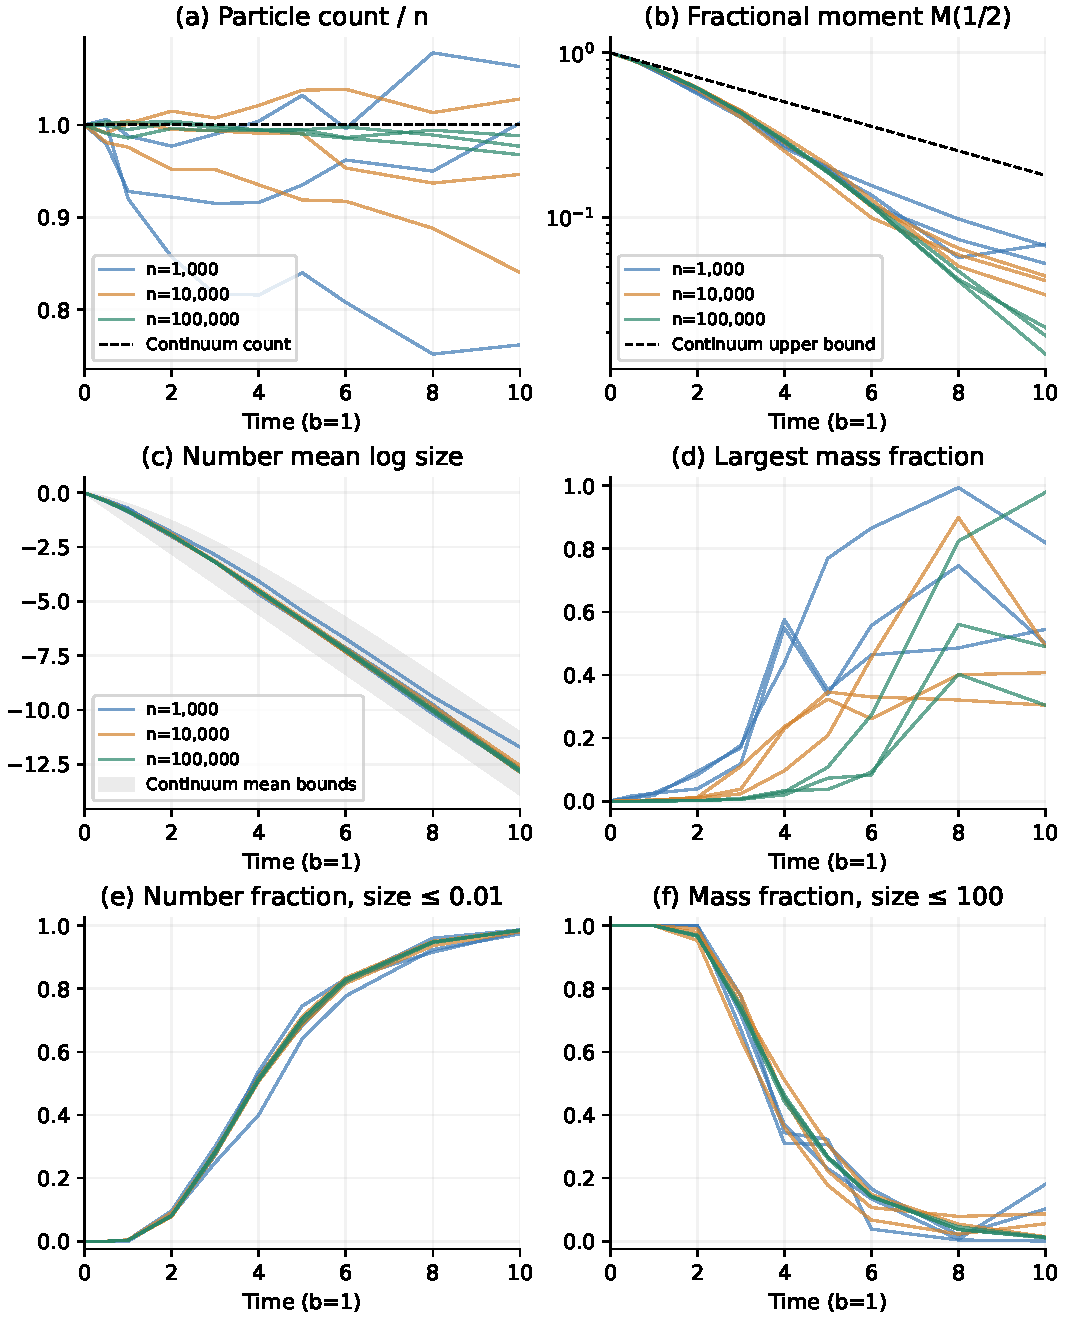
\includegraphics[width=\textwidth,height=.86\textheight,keepaspectratio]{supplement/critical_additive_particles.pdf}
 \caption{All nine finite-particle runs, with three seeds in each color.
 The dashed count and half-moment curves and the shaded mean-log interval
 are continuum references, not pathwise finite-system bounds. Number
 fractions and log means use the actual count $L$; mass fractions use total
 physical mass $n$; $M_{1/2}=n^{-1}\sum_i\sqrt{x_i}$. The figure is generated
 directly from the supplied 90-row CSV.}
 \label{fig:finite-particles}
\end{figure}

\begin{table}[tbp]
 \centering\small
 \begin{tabular}{@{}rrrrr@{}}
 \toprule
 Initial $n$ & $L(10)/n$ & $M_{1/2}(10)$ & Largest mass fraction
 & Number fraction $x\leq0.01$\\
 \midrule
 $10^3$ & $0.762$--$1.063$ & $0.0525$--$0.0688$ & $0.500$--$0.820$ & $0.974$--$0.987$\\
 $10^4$ & $0.8405$--$1.028$ & $0.0339$--$0.0441$ & $0.304$--$0.492$ & $0.981$--$0.986$\\
 $10^5$ & $0.96772$--$0.98823$ & $0.0148$--$0.0215$ & $0.304$--$0.979$ & $0.985$--$0.986$\\
 \bottomrule
 \end{tabular}
 \caption{Minima and maxima over the three declared seeds at time 10.
 These ranges are descriptive, not confidence intervals.}
 \label{tab:finite-particles}
\end{table}

\Cref{fig:finite-particles,tab:finite-particles} show number concentration
near small sizes alongside highly variable material concentration in a few
large particles. At time 10 the count is within $3.3\%$ of its continuum
value for $n=10^5$. The largest absolute relative deviations for $n=10^3$
and $n=10^4$ are $23.8\%$ and $15.95\%$, respectively. The run with
$n=10^4$, seed 47, ends $3.59$ exact standard deviations
below its count mean and is included without selection. Three seeds do not
reliably estimate the count distribution or mass-tail variability. The
dashed half-moment reference is the continuum bound $e^{-\kappa t}$, equal
to $0.17983$ at time 10; the shaded mean-log interval is
$[-2t\log2,\,-2t\log2+(1-e^{-2\kappa t})/(2\kappa)]$ from
\cref{thm:transport} and the half-moment estimate. All nine finite log means
fall inside this interval, but that fact does not turn the interval into a
stochastic bound. The mass-discrepancy certificate of
\cref{thm:finite-discrepancy} at this horizon is about $1.95\times10^{-5}$
for $n=10^3$ and zero for the two larger sizes, whose threshold times
$\log n/\log2$ are $9.97$, $13.29$, and $16.61$ (\cref{rem:finite-constant}).
These runs therefore neither establish a nearly maximal continuum
discrepancy nor measure a first breakdown time.

The half-moment panel does give a rough empirical decay rate. For the
finite system write $A_{1/2}(t)=M_{1/2}(\mu_t^n)$. The fitted rate
$-\log(A_{1/2}(10)/A_{1/2}(4))/6$ on $t\in[4,10]$, computed from the saved
CSV, is listed in \cref{tab:finite-decay}. It is $0.23$--$0.28$ for
$n=10^3$, $0.30$--$0.37$ for $n=10^4$, and $0.43$--$0.50$ for $n=10^5$,
increasing with $n$, against the certified continuum coefficient
$\kappa=3-2\sqrt2\approx0.172$. This supports the conjecture in
\cref{rem:exponent-conjecture} that the true critical exponent for these
data is near $b/2$. The caveats are finite-size effects, including the
ceiling and the $1/n$ correction \eqref{eq:finite-diagonal}, and only three
seeds per size.

\begin{table}[tbp]
 \centering\small
 \begin{tabular}{@{}rrrr@{}}
 \toprule
 Initial $n$ & Seed 11 & Seed 29 & Seed 47\\
 \midrule
 $10^3$ & $0.228$ & $0.275$ & $0.236$\\
 $10^4$ & $0.311$ & $0.368$ & $0.302$\\
 $10^5$ & $0.496$ & $0.432$ & $0.455$\\
 \bottomrule
 \end{tabular}
 \caption{Fitted decay rate $-\log(A_{1/2}(10)/A_{1/2}(4))/6$ of the finite
 half moment on $t\in[4,10]$ with $b=1$, from the saved CSV. The certified
 continuum coefficient is $\kappa\approx0.172$.}
 \label{tab:finite-decay}
\end{table}

The self-contained supplement includes the C++ source, standard-library
Python runner, recorded data and compiler metadata, figure script, and
build commands. Built-in checks exercise selection intervals, resizing,
removal, pair rates, count-generator identities, and conservation over
10,000 events. Each snapshot checks $L=n+\mathrm{births}-\mathrm{deaths}$,
the mass ceiling, and agreement of direct and tree mass sums, with relative
mass tolerance $10^{-10}$. The archived normalized mass is printed as one
at every snapshot. Equal splitting preserves dyadic masses in real
arithmetic, but a bound on their size range does not bound the number of
significant bits needed for exact arithmetic. Floating-point rounding can
occur in merges and cumulative sums even in these runs; the printed mass
values do not certify exact conservation. Longer runs with extreme size
ratios can lose small weights in cumulative sums, and the uniform draws
have 53 bits of resolution. Different
floating-point platforms or C++ library implementations can change a path
with the same seed. The supplement also records the prior independent
structural and count-law checks and their reproducible commands; they are
implementation diagnostics, not extra research trajectories.

\section{What bulk observables hide, and what fails beyond the additive kernel}
\label{sec:boundaries}

Count neutrality has an exact algebraic classification at fixed mass. It
explains why constant count, mass, and mean size can coexist with rapid
broadening. A second observable removes this universal ambiguity. Beyond
the additive kernel, the same classification also leads to a finite-count
nonstationarity theorem, while fractional-moment monotonicity can fail.

\subsection{Universal count neutrality and observable rigidity}

In this subsection $K:E^2\to[0,\infty)$ is measurable, symmetric and finite
pointwise, and $S:E\to[0,\infty)$ is measurable and finite pointwise. The
expected daughter measure $b_x$ satisfies \eqref{eq:daughters}. For a
finitely supported preparation $v$, define its count vector field by
\[
 \mathcal R(v)=\int S(x)v(\dd x)-\frac12\iint K(x,y)v(\dd x)v(\dd y).
\]
This definition concerns initial rates and needs no existence theorem for
the general kernel. Fix a prescribed material mass $m>0$. The preparation
class below fixes this mass while allowing count to vary.

\begin{theorem}[The complete count-neutral class]\label{thm:neutral-class}
The identity $\mathcal R(v)=0$ holds for every nonnegative finitely
supported $v$ with $M_1(v)=m$ if and only if there is a nonnegative
measurable function $d$, finite pointwise, such that
\begin{equation}
 K(x,y)=xd(y)+yd(x),\qquad S(x)=md(x).
 \label{eq:neutral-class}
\end{equation}
For this class, any mass-conserving trajectory at mass $m$ whose weak count
balance has locally integrable event rates has constant count.
\end{theorem}

\begin{proof}
The preparation $(m/x)\delta_x$ gives
$S(x)=mK(x,x)/(2x)$. Define $d(x)=S(x)/m$. For $x\ne y$, substitute
$v=(m/(2x))\delta_x+(m/(2y))\delta_y$ and use the diagonal identities.
After cancellation the result is $K(x,y)=xd(y)+yd(x)$; the same relation
already holds on the diagonal. Conversely, for \eqref{eq:neutral-class},
\begin{equation}
 \mathcal R(v)=(m-M_1(v))\int d(x)v(\dd x).
 \label{eq:neutral-count-balance}
\end{equation}
This proves the equivalence. Along a trajectory with the stated event
integrability, the weak count balance integrates the right-hand side of
\eqref{eq:neutral-count-balance}, which vanishes by mass conservation.
\end{proof}

The full-time assertion uses the weak equation and conserved mass, rather
than inferring a trajectory from an initial derivative. The fixed-mass
preparation class is essential: a class fixing both mass and count admits
only one monodisperse size and cannot support the proof below.

\begin{proposition}[An additional moment forces zero kinetics]
\label{prop:observable-rigidity}
Fix any $0<p<1$. If the count vector field vanishes for every finitely
supported preparation of mass $m$, and the $p$th-moment vector field
vanishes for every monodisperse preparation of mass $m$, then
$K=S=0$ pointwise. The same conclusion holds if the second moment replaces
the $p$th moment. In particular one may use the half moment.
\end{proposition}

\begin{proof}
By \cref{thm:neutral-class}, the rates have form \eqref{eq:neutral-class}
with $d\geq0$. At $v=(m/x)\delta_x$ the coagulation contribution to the
$p$th-moment vector field is
$m^2d(x)x^{p-1}(2^p-2)$. Jensen's inequality bounds fragmentation by
$m^2d(x)x^{p-1}(2^{1-p}-1)$. Therefore their sum is at most
\begin{equation}
 -\kappa_p m^2d(x)x^{p-1}.
 \label{eq:rigidity-fractional}
\end{equation}
If this vector field is zero, then $d(x)=0$ for every $x$.
For the second moment, Jensen gives
$\int z^2b_x(\dd z)\geq x^2/2$, so the corresponding vector field is
at least $3m^2xd(x)/2$. Its universal vanishing again forces $d=0$.
Every displayed integral is finite for these monodisperse preparations
because daughters lie below their parent.
\end{proof}

This is a result about a class of preparations at fixed mass, not
identification of arbitrary rates from a single observed trajectory.
Only monodisperse preparations enter the moment hypothesis, and the proof
of \cref{thm:neutral-class} uses only preparations with at most two atoms,
so the count hypothesis can be weakened to that class as well. Nonnegative
physical rates are used in the conclusion from
\eqref{eq:rigidity-fractional}.

\subsection{Broadening and entropy production with fixed bulk outputs}

Return to the additive member $d\equiv\lambda>0$, with critical selection
$b=\lambda m$. The daughter law may now depend measurably on time and size,
as in \cref{ass:rates}. In the finite-second-moment solution class already
constructed, second-moment and entropy balances require no extra assumptions.
Use $\mathcal H(t)=\int x\log x\,n_t(\dd x)$ for the entropy moment, to
avoid confusing it with the half moment $H$ used earlier.

\begin{proposition}[Two unbounded observables]\label{prop:broadening-entropy}
For the critical solution of \cref{thm:existence}, $M_2$ and $\mathcal H$
are finite and locally absolutely continuous, and almost everywhere
\begin{align}
 \frac32\lambda mM_2(t)&\leq M_2'(t)\leq2\lambda mM_2(t),
 \label{eq:broadening}\\
 \mathcal H'(t)&\geq\lambda m^2\log2.
 \label{eq:entropy-production}
\end{align}
In particular,
\begin{equation}
 M_2(0)e^{3\lambda mt/2}\leq M_2(t)\leq M_2(0)e^{2\lambda mt},
 \qquad
 \mathcal H(t)\geq\mathcal H(0)+\lambda m^2t\log2.
 \label{eq:broadening-integrated}
\end{equation}
Equal splitting gives exactly $M_2(t)=M_2(0)e^{3\lambda mt/2}$.
The entropy production constant is sharp as a uniform instantaneous bound:
monodisperse data with equal splitting attain it at time zero.
\end{proposition}

\begin{proof}
The unbounded-test justification is given in \cref{app:unbounded}; it
establishes the complete integrated weak balances using only locally
bounded $M_2$. The coagulation contribution to $M_2'$ is
$2\lambda mM_2$. By Jensen and $z<x$,
\[
 x^2/2\leq\int z^2b_{t,x}(\dd z)\leq x^2,
\]
so the fragmentation contribution lies between $-bM_2/2$ and zero.
This proves \eqref{eq:broadening} and its equal-split identity.

For $f(x)=x\log x$, put $u=x/(x+y)$ and
$h(u)=-u\log u-(1-u)\log(1-u)$. Then
$\Delta f(x,y)=(x+y)h(u)$. Divide \eqref{eq:pair} by $1-p$ and let
$p\uparrow1$ at fixed positive $x,y$. Differentiability of the scalar powers
gives
\begin{equation}
 (x+y)\Delta f(x,y)\geq4(\log2)xy,
 \quad\text{equivalently}\quad h(u)\geq4(\log2)u(1-u).
 \label{eq:entropy-pair}
\end{equation}
Estimates of this subadditivity type for concave tests are standard in
the coagulation--fragmentation literature; see
\citet{EscobedoMischlerRodriguezRicard2005}.
Thus coagulation produces at least $2\lambda m^2\log2$. Jensen's inequality
for $b_{t,x}/2$ and the increase of $f(z)/z=\log z$ give
\[
 -x\log2\leq\int f(z)b_{t,x}(\dd z)-f(x)\leq0.
\]
Fragmentation loses at most $bm\log2$, proving
\eqref{eq:entropy-production}. Integrating proves
\eqref{eq:broadening-integrated}. Both scalar inequalities are equalities
at a monodisperse equal-split initial state. The right derivative there
is justified at the end of \cref{app:unbounded}, so sharpness is a statement
about actual solutions as well as their vector fields.
\end{proof}

Expected daughter count two and expected daughter mass $x$ suffice for
these bounds; an eventwise binary law is not needed. For any fixed initial
measure with $0<M_2(0)<\infty$, compare the equal-split solution with the
static model $K=S=0$ from that same measure. At every time both models have
identical count $N_0$, mass $m$, and mean size $m/N_0$, yet their second
moments differ by
$M_2(0)(e^{3\lambda mt/2}-1)$. At a fixed positive time this difference
can be made arbitrarily large by increasing $\lambda$. Consequently these
three bulk outputs alone cannot bound the second-moment error uniformly
over the class. For each fixed $\lambda$ the second moment remains finite
at every finite time; this example has no finite-time gelation claim.
The entropy inequality provides another strictly increasing observable in
the same accepted solution class.

\subsection{A power-kernel nonstationarity theorem}

Consider a separate time-independent model,
\begin{equation}
 K(x,y)=xy^\alpha+yx^\alpha,\qquad S(x)=s x^\alpha,
 \qquad 0<\alpha\leq1,\quad s\geq0.
 \label{eq:power-kernel}
\end{equation}
Let $B_x$ be the pushforward of $b_x$ by $z\mapsto z/x$, so
$B_x((0,1))=2$ and $\int\theta B_x(\dd\theta)=1$. These fraction measures
may depend measurably on the parent. A stationary measure means a
nonnegative measure $v$ whose coagulation--fragmentation vector field is
zero for every bounded Borel test, with finite total event integrals.

\begin{theorem}[No finite-count equilibrium for power kernels]
\label{thm:power-no-equilibrium}
For \eqref{eq:power-kernel} and every such daughter law, there is no
stationary measure $v$ with finite positive count $N$ and finite positive
mass $m$. No negative moment, logarithmic moment, or moment above order
one is required.
\end{theorem}

\begin{proof}
Suppose $v$ is such a measure and put $D=M_\alpha(v)$.
The inequality $x^\alpha\leq1+x$ gives $0<D<\infty$; the total coagulation
and fragmentation event rates are $mD$ and $sD$. Testing stationarity
with one gives $(s-m)D=0$, hence $s=m$. The case $s=0$ is already excluded
because $m>0$.

At $s=m$ the integrated population vector field equals
$\int\mathcal Lf\dd v$, where
\begin{equation}
 \mathcal Lf(x)
 =x\int y^\alpha[f(x+y)-f(x)]v(\dd y)
  +mx^\alpha\int[f(\theta x)-f(x)]B_x(\dd\theta).
 \label{eq:power-generator}
\end{equation}
To verify this, symmetry combines the coagulation gains and the two
losses in the full weak field into
$\iint xy^\alpha f(x+y)\dd v\dd v-D\int xf\dd v-m\int x^\alpha f\dd v$.
Fragmentation adds $m\int x^\alpha\int f(\theta x)B_x(\dd\theta)v(\dd x)
-m\int x^\alpha f\dd v$, exactly as in \eqref{eq:power-generator}.
The total jump rate of this representation is
\begin{equation}
 q(x)=xD+2mx^\alpha,
 \qquad \int q(x)v(\dd x)=3mD.
 \label{eq:power-rate}
\end{equation}
Divide its nonnegative gain kernel by $q(x)>0$ to obtain a Markov
transition kernel $P(x,\dd z)$, and set
$\zeta(\dd x)=q(x)v(\dd x)/(3mD)$. Bounded-test stationarity is exactly
the finite-measure identity $\zeta P=\zeta$.

The singular test $g(x)=x^{-\alpha}$ need not be integrable under $v$,
but it is integrable under the rate-weighted probability:
\begin{equation}
 3mD\int g\dd\zeta=D M_{1-\alpha}(v)+2mN<\infty.
 \label{eq:power-singular-integrability}
\end{equation}
Test $\zeta P=\zeta$ first with $g\wedge k$ and let $k\uparrow\infty$.
Monotone convergence gives $\int Pg\dd\zeta=\int g\dd\zeta<\infty$.
Both gain and loss are therefore integrable, and subtraction is legitimate:
\begin{equation}
 \int\mathcal Lg\dd v=0.
 \label{eq:power-singular-balance}
\end{equation}
No jump-process construction or time-dependent population solution has
been used. Even if some daughter inverse moments are initially infinite,
the hypothetical stationary identity forces their integrated gain to be
finite by \eqref{eq:power-singular-integrability}.

Jensen for $B_x/2$ gives
$\int\theta^{-\alpha}B_x(\dd\theta)\geq2^{1+\alpha}$, so fragmentation
in \eqref{eq:power-singular-balance} contributes at least
$2mN(2^\alpha-1)$. Write its coagulation contribution as $-J$, where
\[
 J=\iint xy^\alpha[x^{-\alpha}-(x+y)^{-\alpha}]v(\dd x)v(\dd y)\geq0.
\]
We claim $J\leq\alpha mN$. Symmetrize the integrand, set $r=x+y$ and
$u=x/r$, and denote the symmetrized integrand by $rC_\alpha(u)/2$, where
\[
 C_\alpha(u)=u(1-u)^\alpha(u^{-\alpha}-1)
 +(1-u)u^\alpha((1-u)^{-\alpha}-1).
\]
Concavity of $z^\alpha$ gives
$u^{-\alpha}-1\leq\alpha(u^{-1}-1)$ and the counterpart with $1-u$.
Thus
\[
 C_\alpha(u)\leq\alpha\bigl[(1-u)^{1+\alpha}+u^{1+\alpha}\bigr]
 \leq\alpha.
\]
Integrating $r/2$ gives $mN$, proving the claim. It follows that
\begin{equation}
 \int\mathcal Lg\dd v
 \geq\bigl[2(2^\alpha-1)-\alpha\bigr]mN
 \geq(2\log2-1)\alpha mN>0,
 \label{eq:power-positive-drift}
\end{equation}
contradicting \eqref{eq:power-singular-balance}.
\end{proof}

At $\alpha=1$, $D=m$ and $\zeta=xv/m$ is the mass probability itself.
The embedded transition coagulates with probability $1/3$ by adding an
independent mass-sampled size and fragments with probability $2/3$ using
$B_x/2$. Since $\int x^{-1}\zeta(\dd x)=N/m<\infty$, stationarity would
imply
\[
 3\E(1/X)=\E[1/(X+Y)]+2\E[1/(X\Theta)]\geq4\E(1/X),
\]
a direct contradiction; here $X,Y$ are independent with law $\zeta$ and
$\Theta\mid X$ has law $B_X/2$. This illustrates why rate weighting makes
the singular test admissible.

\subsection{Failure of fractional-moment monotonicity beyond the additive kernel}

The preceding proof does not transfer the additive model's monotone
positive moments. With equal splitting, take
$v_R=\delta_1+R^{-1}\delta_R$, $R>1$, of mass two, and choose $s=m=2$.
Direct substitution gives, for $0<p<1$,
\begin{align}
 \mathcal D_p(v_R)
 &=A_p(1+R^{\alpha+p-1})
 +(1+R^{\alpha-1})[(1+R)^p-1-R^p],\label{eq:power-counterexample}\\
 A_p&=2^p+2^{2-p}-4=\frac{(2^p-2)^2}{2^p}>0.\notag
\end{align}
For verification, the two diagonal coagulation terms are
$(2^p-2)(1+R^{\alpha+p-1})$, fragmentation is
$2(2^{1-p}-1)(1+R^{\alpha+p-1})$, and the cross coagulation term is the
second term in \eqref{eq:power-counterexample}. If $p>1-\alpha$, the first
term tends to infinity, while the negative second term remains bounded:
$-1<(1+R)^p-R^p-1<0$ and $1+R^{\alpha-1}\leq2$.
Nothing is proved for $p\leq1-\alpha$: there the first term stays
bounded and this family does not settle the sign of
$\mathcal D_p(v_R)$.

In particular the half moment can have positive drift for every
$\alpha>1/2$. An explicit half-moment counterexample is $\alpha=1$, $p=1/2$, $R=64$:
\begin{equation}
 \mathcal D_{1/2}(v_{64})=27\sqrt2+2\sqrt{65}-54
 >\frac{151}{500}>0.
 \label{eq:power-half-positive}
\end{equation}
Indeed $(1414/1000)^2<2$ and $(8062/1000)^2<65$, and substitution gives
the rational lower bound. The supplement independently evaluates the
atomic double sum and certifies this inequality by rational arithmetic.
These are vector-field counterexamples. If a local mass-conserving solution
with the required initial moment derivative is separately established,
they give that derivative; no time-dependent existence assertion for
\eqref{eq:power-kernel} is made here. Since count and mass are neutral at
these data, the same sign obstruction applies to a universal initial decay
inequality for the normalized affinity.

The finite-count qualification is necessary. \citet[Proposition 4.3 and
Remark 4.4 of arXiv version 3, whose numbering we follow]{TranVan2022}
construct critical stationary
Bernstein transforms for $K(x,y)=xy$ and a constant binary breakup kernel,
which in our notation means selection $x/2$ and uniform daughter fractions.
Their mass-one convention maps to $K=2xy$, $S=mx$ at mass $m$ by
$n_t=m c_{2mt}$. Writing their stationary transform as
$F(q)=\int(1-e^{-qx})c(\dd x)$ and $G=1-F'$, their identity is
\[
 \frac{G(q)}{(1-G(q))^3}=Cq,\qquad C>0.
\]
It implies $F'(0)=1$ and
$F(q)\sim\tfrac32C^{-1/3}q^{2/3}\to\infty$: indeed $G(q)\to1$ and
$F'(q)=1-G(q)\sim(Cq)^{-1/3}$, which can be integrated using two-sided
asymptotic bounds. Monotone convergence in the Bernstein representation
then gives infinite count. These known equilibria do not contradict
\cref{thm:power-no-equilibrium}.

For $0<\alpha\leq1$, that theorem establishes only stationary exclusion.
It does not supply mass conservation, boundary convergence, logarithmic
scaling, or a final auxiliary coagulation event for time-dependent power
kernels. For $\alpha>1$, both the finite flux and the concavity estimate in
its proof can fail under count and mass assumptions alone; that regime is
outside the result.

\section{Late-time Fourier identification and a pointwise sampling bound}
\label{sec:fourier}

Throughout this section $\lambda>0$ and $\sigma\geq0$ are constants,
$b=\lambda m$, and the selfsimilar daughter measure in
\eqref{eq:selfsimilar-daughters} is a fixed measure $B$. Thus
$B((0,1))=2$ and $\int\theta B(\dd\theta)=1$.
We assume a solution in \cref{def:solution}; no initial or daughter
logarithmic moment is required. The well-posed class in
\cref{thm:existence} supplies such solutions when $M_2(0)<\infty$.
Define the log-size characteristic function and fragmentation exponent by
\begin{equation}
 \chi_t(k)=\int_E e^{ik\log x}\eta_t(\dd x),\qquad
 \psi(k)=\sigma\int_{(0,1)}(\theta^{ik}-1)B(\dd\theta),
 \quad k\in\R.
 \label{eq:fourier-def}
\end{equation}
The symbol $\chi_t$ is a log-size characteristic function, not a
raw-size Laplace transform.
The exponent $\psi$ is continuous, vanishes at zero, and has nonpositive
real part. Its finite jump measure is
$\nu=\sigma(\log)_\# B$, supported on $(-\infty,0)$.

Fourier and Mellin inversion are established tools for fragmentation
inference. The exact pure-fragmentation transform evolution appears in
\citet[equations (12)--(14)]{DoumicEscobedo2016}; inverse recovery from
asymptotic profiles and from short-time observations is developed by
\citet{DoumicEscobedoTournus2018,DoumicEscobedoTournus2024}.
Most directly, \citet[Section 2.2]{Garnier2024} cancels an unknown factor
with two-time characteristic-function quotients and uses a distinguished
logarithm for decompounding. Here the task is to justify this cancellation
asymptotically in a nonlinear equation and bound the coagulation error.
The limiting factor need not be a characteristic function.
\citet[Sections 3.1.1--3.1.4]{HoangEtAl2022} already develops
log-size Fourier estimation from independent samples of an asymptotic
growth--fragmentation profile, including denominator regularization.
That model has size growth and division without coagulation.

\subsection{Factorization with an exponentially small nonlinear error}

Set, consistently with \eqref{eq:constant-log-parameters},
\begin{equation}
 \omega=\kappa(b+\sigma)>0,\qquad
 a_0=\frac{\lambda H(0)^2}{N_0},\qquad
 \delta(k)=\omega+\operatorname{Re}\psi(k),\qquad
 \Xi(k)=\frac{|k|a_0}{\delta(k)}\quad(\delta(k)>0).
 \label{eq:fourier-constants}
\end{equation}
The condition $\delta(k)>0$ defines an admissible frequency set containing
a neighborhood of zero; it can have several connected components.
Since $1-\cos u\leq u^2/2$,
\begin{equation}
 \operatorname{Re}\psi(k)
 \geq-\frac{\sigma k^2}2\int_{(0,1)}(\log\theta)^2B(\dd\theta),
 \label{eq:window-quadratic}
\end{equation}
so if $\sigma>0$ and the fraction law has a finite second logarithmic
moment, the set $\{\delta>0\}$ contains
\begin{equation}
 |k|<\left(\frac{2\omega}{\sigma\int(\log\theta)^2B(\dd\theta)}\right)^{1/2}.
 \label{eq:window}
\end{equation}
When $\sigma=0$, the set is all of $\R$. At criticality with equal
splitting, $\sigma=b$, $\omega=2\kappa b$, and
$\int(\log\theta)^2B(\dd\theta)=2(\log2)^2$, so \eqref{eq:window} reads
$|k|<\sqrt{2\kappa}/\log2\approx0.85$. In this case
$\operatorname{Re}\psi(k)=2b[\cos(k\log2)-1]$. With
$\theta_0=\arccos(1-\kappa)$, the full admissible set is therefore
\[
 \{k:\delta(k)>0\}
 =\bigcup_{j\in\mathbb Z}
 \left(\frac{2\pi j-\theta_0}{\log2},
       \frac{2\pi j+\theta_0}{\log2}\right).
\]
Its component containing zero is $|k|<\theta_0/\log2\approx0.86$.
These bands certify factorization; the nonvanishing amplitude needed for
quotient identification is guaranteed below only on a neighborhood of zero.
The admissible set is inherited from the rate $\omega$ in
\eqref{eq:half-decay}, whose asymptotic optimality is not asserted.
The factorization may hold at more frequencies, but it is proved only
where $\delta>0$.

\begin{theorem}[Nonlinear Fourier factorization]\label{thm:factorization}
For every real $k$ with $\delta(k)>0$, there is an amplitude
$C_\infty(k)$ such that, for all $t\geq0$,
\begin{align}
 |\chi_t(k)-e^{t\psi(k)}C_\infty(k)|
 &\leq \Xi(k)e^{-\omega t},\label{eq:factorization}\\
 |e^{-t\psi(k)}\chi_t(k)-C_\infty(k)|
 &\leq \Xi(k)e^{-\delta(k)t}.\label{eq:amplitude-error}
\end{align}
The set $\{\delta>0\}$ is open and contains zero, and $C_\infty$ is
continuous on it. There is a compact interval $I$ with zero in its
interior on which $\delta$ and $|C_\infty|$ are bounded below by positive
constants. Also $C_\infty(0)=1$.
\end{theorem}

\begin{proof}
Use the real and imaginary parts of $e^{ikz}$ in
\eqref{eq:normalized-log}. In the locally absolutely continuous sense,
\begin{align}
 \partial_t\chi_t(k)&=\psi(k)\chi_t(k)+r_t(k),\notag\\
 r_t(k)&=\frac\lambda{N(t)}\iint x
  [e^{ik\log(x+y)}-e^{ik\log x}]n_t(\dd x)n_t(\dd y).
 \label{eq:fourier-source}
\end{align}
The paired increment bound
$|e^{iku}-e^{ikv}|\leq|k||u-v|$ and
$\log(1+y/x)\leq\sqrt{y/x}$ give, by \eqref{eq:half-decay},
\begin{equation}
 |r_t(k)|\leq |k|\frac{\lambda H(t)^2}{N(t)}
             \leq |k|a_0e^{-\omega t}.
 \label{eq:fourier-forcing}
\end{equation}
Variation of constants therefore defines the absolutely convergent integral
\begin{equation}
 C_\infty(k)=\chi_0(k)+\int_0^\infty e^{-s\psi(k)}r_s(k)\dd s.
 \label{eq:fourier-amplitude}
\end{equation}
Subtracting its tail proves \eqref{eq:amplitude-error}; multiplying by
$e^{t\operatorname{Re}\psi(k)}$ proves \eqref{eq:factorization}.
Since $\psi$ is continuous with $\psi(0)=0$, the set $\{\delta>0\}$ is
open and contains zero. On each compact subset of it, $\delta$ is bounded
below by a positive constant and $\Xi$ is bounded, so
$e^{-t\psi}\chi_t$, which is continuous in $k$, converges uniformly to
$C_\infty$ by \eqref{eq:amplitude-error}. Thus the amplitude is
continuous on $\{\delta>0\}$. At zero it equals one, so a compact
neighborhood of zero gives the nonvanishing.
\end{proof}

The amplitude includes both the unknown initial law and the accumulated
nonlinear interactions. Equation \eqref{eq:fourier-amplitude} gives no
independence interpretation for it and does not assert positive
definiteness. The notation distinguishes it from the controlled clock
$C(t)$ in \eqref{eq:clocks}.

\subsection{Exact-data identification from local frequencies}

\begin{corollary}[Late-time quotients]\label{cor:fourier-ratio}
Let $I$ be the interval of \cref{thm:factorization}. Then
$\chi_t(k)\ne0$ for all sufficiently large $t$, uniformly in $k\in I$,
and for every $h>0$
\begin{equation}
 R_t(k):=\frac{\chi_{t+h}(k)}{\chi_t(k)}
       \longrightarrow e^{h\psi(k)}
 \label{eq:ratio-limit}
\end{equation}
uniformly on $I$. Whenever
$\Xi(k)e^{-\delta(k)t}\leq|C_\infty(k)|/2$,
\begin{equation}
 |R_t(k)-e^{h\psi(k)}|
 \leq \frac{2\Xi(k)}{|C_\infty(k)|}
 e^{h\operatorname{Re}\psi(k)}(1+e^{-\delta(k)h})e^{-\delta(k)t}.
 \label{eq:ratio-bias}
\end{equation}
Fix $h>0$. There is a compact interval $I'\subset I$ with zero in its
interior on which the continuous logarithm of the limiting quotient,
anchored at zero by $\log 1=0$, recovers $\psi$:
\begin{equation}
 \psi(k)=\frac1h\log\!\left(\lim_{t\to\infty}R_t(k)\right),
 \qquad k\in I'.
 \label{eq:local-exponent}
\end{equation}
\end{corollary}

\begin{proof}
Write $e^{-t\psi(k)}\chi_t(k)=C_\infty(k)+\epsilon_t(k)$.
The denominator has modulus at least $|C_\infty(k)|/2$ under the
stated condition. Subtract $e^{h\psi(k)}$ from the quotient and bound
$|\epsilon_{t+h}(k)-\epsilon_t(k)|$ using
\eqref{eq:amplitude-error}. Uniform bounds on $\Xi$, $\delta^{-1}$,
and $|C_\infty|^{-1}$ on $I$ give the uniform conclusion.
Choose $I'\subset I$ so small that $e^{h\psi(k)}$ stays near one and
$|h\operatorname{Im}\psi(k)|<\pi$ on $I'$. The principal logarithm there
is continuous and equals $h\psi(k)$; equivalently it is the unique
continuous branch anchored at zero.
\end{proof}

The interval $I$ depends on the kinetics and the initial data through
$\omega$, $a_0$, and the lower bound for $|C_\infty|$; the interval $I'$
depends in addition on $h$. These quantities are unknown in an
identification problem, and no computable procedure for choosing $I$ or
$I'$ from observations is offered here. The corollary is a proof of
principle.

For completeness, the analytic uniqueness ingredient needs no log moments.
It is the classical uniqueness theorem for boundary values of bounded
holomorphic functions in a half-plane, in a Paley--Wiener-type form: the
transform of a finite measure on a half-line extends to a bounded
holomorphic function in a half-plane, and a bounded holomorphic function
whose boundary values vanish on a set of positive length is identically
zero (a theorem of F.\ and M.\ Riesz, extended by Lusin and Privalov).
Continuity up to the boundary allows the short reflection proof below.

\begin{lemma}[One-sided transform uniqueness]\label{lem:one-sided}
Let $\nu_1,\nu_2$ be finite measures on $(-\infty,0)$. If
\[
 \int(e^{iky}-1)\nu_1(\dd y)
 =\int(e^{iky}-1)\nu_2(\dd y)
\]
on a nonempty open real interval, then $\nu_1=\nu_2$.
\end{lemma}

\begin{proof}
Put $\Delta=\nu_1-\nu_2$ and
$\mu=\Delta-\Delta(\R)\delta_0$. This is a finite signed measure
supported on $(-\infty,0]$, and its Fourier transform vanishes on the
specified interval. The function
\[
 f(z)=\int e^{izy}\mu(\dd y),\qquad \operatorname{Im}z<0,
\]
is holomorphic in the lower half-plane and continuous up to the real
boundary. Indeed, the exponential is bounded by one there; on compact
subsets of the open half-plane its damping controls every power of
$|y|$, justifying differentiation without moments.
Its zero boundary values are real. Schwarz reflection across a smaller
segment extends $f$ holomorphically through that segment. The extension
vanishes on the segment, so the identity theorem makes it zero on an
open subset and then throughout the lower half-plane. Boundary
continuity gives a zero Fourier transform on all of $\R$. Uniqueness
of Fourier transforms of finite signed measures yields $\mu=0$.
Restriction to $(-\infty,0)$ gives $\Delta=0$.
\end{proof}

\begin{theorem}[Structural identification]\label{thm:fourier-identification}
Ideal exact knowledge of the normalized size laws at the pairs of times
$(t_j,t_j+h)$, for one fixed lag $h>0$ and some sequence $t_j\to\infty$,
determines $\nu=\sigma(\log)_\#B$ uniquely.
If $\sigma>0$, it determines
\begin{equation}
 \sigma=\tfrac12\nu((-\infty,0)),\qquad
 B=\sigma^{-1}(\exp)_\#\nu.
 \label{eq:daughter-recovery}
\end{equation}
If $\sigma=0$, it identifies the zero selection rate but cannot identify
an unused $B$. With additionally known conserved mass $m$ and observed
unnormalized count growth $r_N$, it determines
\begin{equation}
 r_N=\frac{\log N(t+h)-\log N(t)}h=\sigma-\lambda m,
 \qquad \lambda=\frac{\sigma-r_N}{m}.
 \label{eq:coag-recovery}
\end{equation}
Neither the initial distribution nor its characteristic function needs
to be known.
\end{theorem}

\begin{proof}
Since the limit in \eqref{eq:ratio-limit} exists, the observations along
$t_j$ give \eqref{eq:local-exponent} on the open neighborhood
$\operatorname{int}I'$ of zero. For two candidate models, intersect
their neighborhoods;
\cref{lem:one-sided} identifies their jump measures. Their common total
mass is $2\sigma$, proving \eqref{eq:daughter-recovery} and the zero-rate
case. The count identity \eqref{eq:count} proves
\eqref{eq:coag-recovery}.
\end{proof}

A fixed change of size unit multiplies both $\chi_t$ and $\chi_{t+h}$ by
the same phase, which cancels in their quotient. Unknown initial data
cancel through $C_\infty$. Absolute mass and unnormalized count growth
are separate observations in \eqref{eq:coag-recovery}. The theorem uses
a continuum of exact frequencies in the window $I'$; finitely many
Fourier values do not supply the one-sided uniqueness conclusion, and
the passage from $\psi$ on $I'$ to $\nu$ is an analytic continuation from
a short interval, whose ill-posedness is quantified below. The measure $B$
records expected daughters and does not specify additional correlations
or genealogical information absent from the population balance.
The strict support assumption excludes zero log jumps. If one instead
allows $B$ on $(0,1]$ with the same count and mass constraints, an atom
at one contributes nothing directly to the exponent. It is nevertheless
identified by those constraints. Indeed, the visible measure
$\nu_-:=\sigma(\log)_\#(B|_{(0,1)})$ is determined by
\cref{lem:one-sided}, and
\[
 \sigma=\int_{(-\infty,0)}(1-e^y)\nu_-(\dd y),\qquad
 z:=\sigma B(\{1\})=2\sigma-\nu_-(\R).
\]
The integral has a bounded integrand. For $\sigma>0$ these formulas
recover $B=\sigma^{-1}[(\exp)_\#\nu_-+z\delta_1]$.
Thus strict reduction is not necessary for this algebraic identification
when both daughter constraints are known. The forward solution framework
in this paper retains its stated support assumption.

The holomorphic exponent satisfies the mass identity
$\psi(-i)=\sigma\int(\theta-1)B(\dd\theta)=-\sigma$.
This is an identity for the uniquely determined exponent, not an
instruction to continue noisy observations to a complex argument.
Identification from the window rests on \cref{lem:one-sided}, that is,
on analytic continuation from a short interval, and such continuation is
exponentially ill-posed. Quantitatively, let $g=\psi_1-\psi_2$ for two
admissible models with the same $\sigma$. Then $g$ is holomorphic in the
open lower half-plane, continuous up to the real axis, and bounded there
by $8\sigma$. If $|g|\leq\varepsilon$ on $I'$, the two-constants theorem
gives
\[
 |g(z)|\leq\varepsilon^{\varpi(z)}(8\sigma)^{1-\varpi(z)},
\]
where $\varpi(z)$ is the harmonic measure of $I'$ seen from $z$ in the
lower half-plane. This exponent tends to zero as $z$ approaches any real
frequency outside $I'$, so the data on $I'$ control no real frequency
outside $I'$ without further assumptions. If in addition
$\int\theta^{-a}B(\dd\theta)<\infty$ for some $a>0$, so that both
exponents extend holomorphically to the strip $|\operatorname{Im}z|<a$,
the same theorem in the strip slit along $I'$ gives an exponent that
decays exponentially with the distance from $I'$. The resulting bound
is then informative only up to distances of order
$\log\log(1/\varepsilon)$ from $I'$. The norm discontinuity that follows
is one symptom of this ill-posedness.
In fact, take $p\in(0,1)\setminus\{1/2\}$ and
$B_p=\delta_p+\delta_{1-p}$. As $q\to p$ with the four daughter atoms
distinct, the exponents for $B_q$ converge uniformly on each bounded
real-frequency interval, while
$\norm{B_q-B_p}_{\mathrm{var}}=4$.
Thus inversion to the daughter measure in variation norm is not continuous
under this data norm, even with fixed positive $\sigma$ and both daughter
constraints. This does not exclude stability in weaker metrics or under
additional regularity assumptions, but any such stability must be proved
separately; nothing here supplies it.

\subsection{Independent sampling: a pointwise sampling bound and observation time}

Fix one frequency $k\in I$ and a lag $h>0$. At the predetermined times
$t$ and $t+h$, observe $n$ independent draws from each of the deterministic
continuum number laws $\eta_t$ and $\eta_{t+h}$, with the two samples
also independent. These are hypothetical observations of continuum laws,
not the interacting particles of \cref{sec:finite}, and not auxiliary
paths from \cref{sec:auxiliary}.
Write $U=\chi_t(k)$, $V=\chi_{t+h}(k)$, and let
$\widehat U,\widehat V$ be the corresponding empirical averages of
$e^{ik\log X}$. Put $\widehat R=\widehat V/\widehat U$ when defined.
For $0<\varsigma<1$, set
\begin{equation}
 \varepsilon_n=2\sqrt{\frac{\log(8/\varsigma)}n}.
 \label{eq:sampling-epsilon}
\end{equation}

\begin{proposition}[Pointwise sampling bound for the ratio]\label{prop:ratio-sampling}
With probability at least $1-\varsigma$, both empirical characteristic
function errors are at most $\varepsilon_n$. On this event, whenever
$|\widehat U|>\varepsilon_n$, the exact finite-time ratio is defined and
\begin{equation}
 |\widehat R-R_t(k)|
 \leq\frac{\varepsilon_n(1+|\widehat R|)}
                  {|\widehat U|-\varepsilon_n}.
 \label{eq:observable-certificate}
\end{equation}
Let $\delta=\delta(k)>0$ be as in \eqref{eq:fourier-constants}, so that
$\omega-\delta=-\operatorname{Re}\psi(k)\geq0$. Choose
$\underline C>0$, $\Upsilon<\infty$, and $t_0\geq0$ so that
for $t\geq t_0$,
\begin{equation}
 |U|\geq\tfrac{\underline C}2e^{-(\omega-\delta)t},\qquad
 |R_t(k)-e^{h\psi(k)}|\leq\Upsilon e^{-\delta t}.
 \label{eq:sampling-signal}
\end{equation}
Such constants exist by \cref{thm:factorization,cor:fourier-ratio}.
If additionally $\varepsilon_n\leq(\underline C/4)e^{-(\omega-\delta)t}$,
then on the same event $\widehat U\ne0$ and
\begin{equation}
 |\widehat R-e^{h\psi(k)}|
 \leq\Upsilon e^{-\delta t}
  +\frac{4(2+\Upsilon)}{\underline C}\varepsilon_n e^{(\omega-\delta)t}.
 \label{eq:bias-noise}
\end{equation}
For all sufficiently large $n$, the deterministic schedule
\begin{equation}
 t_n=\frac{\log(1/\varepsilon_n)}\omega
 \label{eq:observation-time}
\end{equation}
satisfies these hypotheses and gives
\begin{equation}
 |\widehat R-e^{h\psi(k)}|
 \leq\left[\Upsilon+\frac{4(2+\Upsilon)}{\underline C}\right]
              \varepsilon_n^{\delta/\omega}
 \label{eq:balanced-ratio}
\end{equation}
with probability at least $1-\varsigma$.
\end{proposition}

\begin{proof}
Hoeffding's bounded-variable inequality \citep{Hoeffding1963}, applied
to each real and imaginary component in $[-1,1]$ at threshold
$\varepsilon/\sqrt2$, and a union bound over all four components give
\[
 \Prob\bigl(|\widehat U-U|>\varepsilon
             \text{ or }|\widehat V-V|>\varepsilon\bigr)
 \leq8e^{-n\varepsilon^2/4}.
\]
Substitute \eqref{eq:sampling-epsilon}. On the resulting event,
$|U|\geq|\widehat U|-\varepsilon_n$, and
\[
 \widehat R-R_t
 =\frac{\widehat R(U-\widehat U)-(V-\widehat V)}U
\]
proves \eqref{eq:observable-certificate}. Under the stronger signal
condition, $|\widehat U|\geq(\underline C/4)e^{-(\omega-\delta)t}$ and
$|R_t|\leq1+\Upsilon$, because $|e^{h\psi(k)}|\leq1$.
Using instead
\[
 \widehat R-R_t
 =\frac{\widehat V-V-R_t(\widehat U-U)}{\widehat U}
\]
gives the second term in \eqref{eq:bias-noise}; add the deterministic
bias. Finally, at \eqref{eq:observation-time} both
$e^{-\delta t_n}$ and $\varepsilon_ne^{(\omega-\delta)t_n}$ equal
$\varepsilon_n^{\delta/\omega}$, so both terms are constant multiples of
this quantity. It tends to zero, which verifies the signal condition
eventually; also $t_n\to\infty$.
\end{proof}

The pointwise sampling bound \eqref{eq:observable-certificate} controls
sampling error to the exact finite-time ratio; the bias in
\eqref{eq:ratio-bias} must still be added to estimate $e^{h\psi(k)}$.
Its strict denominator condition is required. At fixed confidence,
\eqref{eq:balanced-ratio} is an upper bound of order
$n^{-\delta/(2\omega)}$, attained at a time of order
$(\log n)/(2\omega)$. This is a sufficient balance of the proved bounds,
not a minimax result or an optimal experimental-design theorem.
Both the schedule and the exponent use the certified decay coefficient
$\omega=\kappa(b+\sigma)$ for $H^2/N$ in \eqref{eq:half-decay}.
Its asymptotic optimality is not asserted. For the Golovin
benchmark of pure additive coagulation from monodisperse data
\citep{Golovin1963}, $H^2/N$ decays roughly like $e^{-bt}$ up to
polynomial factors, against the certified $\omega=\kappa b\approx0.17b$.
This benchmark shows that a stronger decay estimate can permit an earlier
observation time, but does not prove faster decay throughout the model
class. If a stronger exponential forcing bound is established for a given
model, the balance can be recomputed with that bound. At frequencies with
$\operatorname{Re}\psi(k)<0$, increasing the decay coefficient improves
the resulting sampling exponent $\delta/(2\omega)$.
When $\delta=\omega$, that is, when $\operatorname{Re}\psi(k)=0$, the
sampling term does not grow with time and the same schedule remains
sufficient. The sampling exponent is then already $1/2$, including in the
pure-coagulation benchmark, and a stronger decay bound does not increase
it. The constants depend on unknown kinetics
and initial data; using the schedule requires their relevant values or
prior class bounds. No adaptive choice of time or frequency is proved,
and no computable procedure selects the frequency interval $I$; the
proposition is a proof of principle under a hypothetical observation
model.
A local logarithm separated from its branch cut transfers pointwise ratio
convergence to the exponent, but supplies no full noisy daughter inversion.
The logarithmic observation time in sample size also does not validate
an estimator based on a single finite reactor: the continuum obstruction
in \cref{thm:finite-discrepancy} concerns a different population parameter
and a different observation law.

\section{Discussion}
\label{sec:discussion}

The additive equation can hide persistent kinetics from bulk count,
mass, and mean size while separating number and mass sampling almost
completely. Fractional moments quantify this distinction and also
control a different object: the accumulated nonlinear displacement
of an auxiliary number path. Its finite log correction explains why
fragmentation governs the large-scale logarithmic limits and the
late-time Fourier quotient. Its almost-sure finite coagulation count
is compatible with infinite expected activity because increasingly
rare paths carry large event counts. It is not a statement that the
physical population eventually stops coagulating.

Several qualifications are part of the mathematical conclusions.
The moment coefficients are sharp only as instantaneous uniform
constants; the Golovin--Borel solution and the archived critical
simulations decay several times faster, so the estimates are Lyapunov
bounds rather than rates. The equal-split daughter envelopes and
overlap constants are extremal over their stated classes, but the
critical calendar-time exponent of the last-coagulation tail is not
determined. The envelopes reduce that exponent to the decay rate of
the deterministic number--mass overlap, a question about the equation
alone, and the simulations suggest the value $b/2$. Proving that rate,
or any asymptotic rate for the fractional moments at criticality, is
the main open problem this paper leaves.
Parent-dependent daughters retain the controlled path bounds, but
do not yield the independent translation-invariant fragmentation
reference without additional structure.

The finite-population statement shows that checking count alone can
miss a nearly maximal error in the material distribution. Its particle
input is only the material ceiling of a finite vessel, so it is a
corollary of the moment bound. It gives a sufficient logarithmic
horizon for this failure, and does not identify the first failure time or prove accuracy
before it. The exact count
law, its later diffusion limit, and the retained simulations answer
different questions from propagation of a full size distribution.
A growing-time approximation for specific bounded statistics would
require a separate argument adapted to those statistics.

The inverse application likewise separates exact identifiability
from stable estimation. A nonvanishing local amplitude cancels the
unknown initial law, and one-sided support determines the jump measure
from exact frequencies on a short low-frequency interval; that step is
analytic continuation and is severely ill-posed. The empirical sampling
bound makes attenuation of the denominator explicit and provides a
sufficient balance between coagulation bias and sampling noise, at a
certified rate whose asymptotic optimality is not asserted. It neither adapts
the observation time to unknown kinetics nor supplies stable analytic
continuation. Establishing recovery of an entire daughter law from noisy
data requires additional assumptions and regularization. Connecting
such an estimator to measurements in a finite vessel also requires an
observation model that accounts for particle dependence and continuum
error. These are distinct tasks beyond the factorization proved here.

The preparation algebra in the supplementary note offers a
complementary lesson:
what can be identified depends on which preparations and observables
are available. Preserving material loading does not remove the complete
count-neutral family. Same-shape dilution can separate linear and
quadratic initial-rate terms when coefficients remain unchanged, but
an unknown source leaves an additional ambiguity with only two
concentrations. Distributional information, physical preparation
constraints, and the sampling law must therefore be specified together.

\appendix
\section{Existence and uniqueness for measurable daughter kernels}
\label{app:existence}

This appendix proves \cref{thm:existence}. In addition to providing a
solution class for the estimates in the paper, the argument explains why
mere measurability of the parent-dependent daughter law causes no gap.
All the approximations converge in weighted variation, which controls
bounded measurable tests directly.

\subsection{Weak kernel integrals and a comparison lemma}

Throughout this appendix, $w(x)=1+x$, so that
$\norm{\mu}_w=\int w\dd|\mu|$ is the weighted variation \eqref{eq:variation}.
If $G_t$ is a signed measure kernel with
$\int_0^T\norm{G_t}_w\dd t<\infty$, its integral is the measure defined
on Borel sets by integration in time. Countable additivity follows from
dominated convergence for the variation kernels, and
\begin{equation}
 \norm{\int_s^tG_u\dd u}_w\leq\int_s^t\norm{G_u}_w\dd u.
 \label{eq:kernel-integral}
\end{equation}
The same convention applies to other positive weights.
This construction does not require strong measurability of $G_t$ as a
Banach-space-valued function. For instance, $t\mapsto\delta_t$ need not
be strongly measurable in total variation, even though all its time
integrals on Borel sets are well defined. We therefore use weak kernel
integrals, rather than a Bochner differential equation on measures.

We first establish the norm estimate used below. Suppose a signed
measure curve $d_t$ satisfies, in weak kernel form,
\begin{equation}
 d_t=d_0+\int_0^t\{H_s-a_s d_s\}\dd s,
 \label{eq:signed-loss}
\end{equation}
where $a_s(x)\geq0$ is jointly measurable and, for every finite $R,T>0$,
there is a nonnegative $h_{R,T}\in L^1(0,T)$ such that
$\sup_{0<x\leq R}a_s(x)\leq h_{R,T}(s)$ for almost every $s\in(0,T)$.
Assume also that $t\mapsto d_t(A)$ is measurable for each Borel $A$ and
that both $H_s$ and $a_sd_s$ have integrable weighted variation on $(0,T)$.
The loss integrating factor gives
\begin{equation}
 d_t(\dd x)=e^{-\int_0^t a_u(x)\dd u}d_0(\dd x)
   +\int_0^t e^{-\int_s^t a_u(x)\dd u}H_s(\dd x)\dd s.
 \label{eq:loss-duhamel}
\end{equation}

Here is the proof. By Tonelli's theorem, $(s,x)\mapsto\int_s^ta_u(x)\dd u$
is jointly measurable, and it is finite for every $x$ because
$a_\cdot(x)\leq h_{x,T}$ on $(0,T)$. The exponential factors are therefore
Borel functions with values in $[0,1]$, and the right-hand side of
\eqref{eq:loss-duhamel} is a finite signed measure on $E$.

Variations of setwise measurable curves are measurable in time, by a
countable supremum: if $t\mapsto\rho_t(A)$ is measurable for each Borel
$A$, then for every Borel $A$ and bounded Borel $\phi\geq0$,
\begin{equation}
 \int_A\phi\dd|\rho_t|
 =\sup_{B\in\mathcal B_0}\Bigl[\int_{A\cap B}\phi\dd\rho_t
                          -\int_{A\setminus B}\phi\dd\rho_t\Bigr],
 \label{eq:variation-countable-sup}
\end{equation}
where $\mathcal B_0$ is the countable algebra of finite unions of intervals
with rational endpoints. Indeed each bracket is at most the left side,
and the Hahn sets of $\phi\rho_t$ are approximated in
$\phi|\rho_t|$-measure by sets from the generating algebra $\mathcal B_0$.
Monotone convergence in $\phi$ extends this to unbounded Borel
$\phi\geq0$, in particular to $\norm{\rho_t}_w$.

Fix $R,T$ and restrict the output coordinate to $(0,R]$: for Borel
$A\subset(0,R]$, \eqref{eq:signed-loss} reads
$d_t(A)=d_0(A)+\int_0^t\{H_s(A)-(a_sd_s)(A)\}\dd s$. The restriction
applies only to the output coordinate; it does not discard any
contribution to $H_s$ from outside that set. Two facts follow from the
assumptions. First, the restricted curve is bounded in variation:
by \eqref{eq:kernel-integral} with weight one,
$\sup_{t\leq T}|d_t|((0,R])\leq\norm{d_0}_w
+\int_0^T(\norm{H_s}_w+\norm{a_sd_s}_w)\dd s<\infty$.
Second, on $(0,R]$ the loss is a multiplication operator bounded by an
integrable function: $|a_s\rho|((0,R])\leq h_{R,T}(s)|\rho|((0,R])$ for
every finite signed measure $\rho$ on $(0,R]$ and almost every $s$.
Consider the linear Volterra equation
\begin{equation}
 \rho_t(A)=d_0(A)+\int_0^tH_s(A)\dd s-\int_0^t(a_s\rho_s)(A)\dd s,
 \qquad A\subset(0,R]\ \text{Borel},\quad t\leq T,
 \label{eq:restricted-volterra}
\end{equation}
in the class of curves $\rho$ of finite signed measures on $(0,R]$ such
that $t\mapsto\rho_t(A)$ is measurable for each Borel $A$ and
$\sup_{t\leq T}|\rho_t|((0,R])<\infty$. The restriction of $d$ belongs to
this class and solves \eqref{eq:restricted-volterra}. Uniqueness holds in
this class: the difference $\delta$ of two solutions satisfies
$\delta_t=-\int_0^ta_s\delta_s\dd s$, hence
$|\delta_t|((0,R])\leq\int_0^th_{R,T}(s)|\delta_s|((0,R])\dd s$, and the
bounded function $s\mapsto|\delta_s|((0,R])$, measurable by
\eqref{eq:variation-countable-sup}, vanishes identically by Gronwall's
inequality. For existence, let $\rho_t$ be the restriction to $(0,R]$ of
the right-hand side of \eqref{eq:loss-duhamel}. It is a finite signed
measure with $|\rho_t|((0,R])\leq|d_0|(E)+\int_0^T|H_s|(E)\dd s$, and
$t\mapsto\rho_t(A)$ is measurable as an integral of a jointly measurable
integrand. For Borel $A\subset(0,R]$, the scalar identity
\[
 \int_r^ta_s(x)e^{-\int_r^sa_u(x)\dd u}\dd s=1-e^{-\int_r^ta_u(x)\dd u},
\]
valid because $a_\cdot(x)$ is integrable on $(0,T)$, and Fubini's theorem,
applicable because the integrands are dominated by $h_{R,T}(s)|d_0|(A)$
and $h_{R,T}(s)|H_r|(A)$, give
\begin{align*}
 \int_0^t(a_s\rho_s)(A)\dd s
 &=\int_A\bigl[1-e^{-\int_0^ta_u(x)\dd u}\bigr]d_0(\dd x)
  +\int_0^t\int_A\bigl[1-e^{-\int_r^ta_u(x)\dd u}\bigr]H_r(\dd x)\dd r\\
 &=d_0(A)+\int_0^tH_r(A)\dd r-\rho_t(A).
\end{align*}
So $\rho$ solves \eqref{eq:restricted-volterra}, and by uniqueness
$\rho_t$ is the restriction of $d_t$ to $(0,R]$. Since both sides of
\eqref{eq:loss-duhamel} are finite signed measures on $E$, letting
$R\to\infty$ through the integers and using countable additivity gives
the identity on every Borel set. This proves \eqref{eq:loss-duhamel}
for every curve $d$ satisfying the assumptions of this paragraph; in
particular, uniqueness is asserted among setwise measurable curves of
finite signed measures whose restrictions to bounded sets are bounded in
variation on bounded time intervals.

Define the nonnegative majorant
\begin{equation}
 z_t(\dd x)=e^{-\int_0^t a_u(x)\dd u}|d_0|(\dd x)
   +\int_0^t e^{-\int_s^t a_u(x)\dd u}|H_s|(\dd x)\dd s.
 \label{eq:z-majorant}
\end{equation}
Then $|d_t|\leq z_t$. Tonelli's theorem and the scalar loss identity
give
\begin{equation}
 \pair{w}{z_t}+\int_0^t\pair{wa_s}{z_s}\dd s
 =\norm{d_0}_w+\int_0^t\norm{H_s}_w\dd s.
 \label{eq:z-balance}
\end{equation}
In particular the integrated loss of $z$ is finite, without any higher
moment assumption on $z$.

\begin{lemma}[Weighted comparison]\label{lem:weighted-comparison}
In the preceding setting, suppose $P_s$ is a positive linear kernel
operator and $r_s$ a signed kernel such that
\begin{equation}
 |H_s|\leq P_s|d_s|+|r_s|,\qquad
 P_s^*w(x)-a_s(x)w(x)\leq c(s)w(x),
 \label{eq:comparison-assumptions}
\end{equation}
where $c\geq0$ is locally integrable, $s\mapsto\pair{P_s^*w-a_sw}{|d_s|}$
is measurable, and all terms paired with $|d_s|$ have finite time
integrals. Then
\begin{equation}
 \norm{d_t}_w\leq e^{\int_0^t c(u)\dd u}
 \left[\norm{d_0}_w+\int_0^t\norm{r_s}_w\dd s\right].
 \label{eq:comparison}
\end{equation}
\end{lemma}

\begin{proof}
Since $z_s\geq|d_s|$, \eqref{eq:z-balance} implies
\begin{align*}
 \norm{d_t}_w
 &\leq\norm{d_0}_w+
 \int_0^t\pair{P_s^*w-a_sw}{|d_s|}\dd s
 +\int_0^t\norm{r_s}_w\dd s\\
 &\leq\norm{d_0}_w+
 \int_0^t c(s)\norm{d_s}_w\dd s+
 \int_0^t\norm{r_s}_w\dd s.
\end{align*}
The function $s\mapsto\norm{d_s}_w$ is measurable by
\eqref{eq:variation-countable-sup} and locally bounded by
\eqref{eq:z-balance}, so Gronwall's inequality yields
\eqref{eq:comparison}.
Thus no differentiation of a norm or of a Hahn sign is needed.
\end{proof}

\subsection{Stability for the additive equation}

Let $n,v$ be two nonnegative curves with locally bounded count and second
moment, satisfying the population equation with the same coefficients,
possibly with an additional signed forcing term $r_t$ in their difference.
Put $d=n-v$ and $\mu=(n+v)/2$. Denote the moments of $\mu$ by
$\bar N,\bar m,\bar M_2$; the two curves need not have equal mass.
Polarization of the quadratic coagulation operator gives, against a test
$f$,
\begin{equation}
 \pair{f}{Q_t(n)-Q_t(v)}
 =\lambda(t)\iint (x+y)\Delta f(x,y)\mu_t(\dd x)d_t(\dd y).
 \label{eq:polarization}
\end{equation}
Write this difference and the fragmentation difference as
$H_t-a_td_t$, where
\begin{equation}
 a_t(y)=\lambda(t)(\bar m(t)+\bar N(t)y)+\sigma(t).
 \label{eq:comparison-loss}
\end{equation}
The terms in $H_t$ are the coagulation gain, the signed cross loss
$-\lambda(t)\mu_t(\dd x)\int(x+y)d_t(\dd y)$, the fragmentation gain,
and $r_t$. Their variations are bounded by $P_t|d_t|+|r_t|$, where
for a nonnegative measure $\xi$ and Borel $A$,
\begin{align}
 (P_t\xi)(A)
 &=\lambda(t)\iint(x+y)
       [\1_A(x+y)+\1_A(x)]\mu_t(\dd x)\xi(\dd y)\notag\\
 &\quad+\sigma(t)\int b_{t,y}(A)\xi(\dd y).
 \label{eq:positive-comparison}
\end{align}
Although the cross loss is replaced by a positive term, keeping the
direct loss $a_td_t$ preserves the cancellation needed for stability:
\begin{align}
 P_t^*w(y)-a_t(y)w(y)
 &=\lambda(t)\int(x+y)[w(x+y)+w(x)-w(y)]\mu_t(\dd x)
       +\sigma(t)\notag\\
 &=\lambda(t)[\bar m+2\bar M_2+y(\bar N+2\bar m)]+\sigma(t)
 \leq c(t)w(y),\label{eq:weight-cancellation}
\end{align}
where we may choose
\begin{equation}
 c(t)=\lambda(t)[\bar N(t)+3\bar m(t)+2\bar M_2(t)]+\sigma(t).
 \label{eq:stability-coefficient}
\end{equation}
All event integrals in weighted variation are finite under the stated
second-moment bounds. For example, the absolute weighted coagulation
increment is bounded by
$(x+y)[w(x+y)+w(x)+w(y)]=(x+y)[3+2(x+y)]$.
Also $a_t(y)\leq\lambda(t)(\bar m(t)+R\bar N(t))+\sigma(t)$ for
$0<y\leq R$, providing the required integrable local bound. The
measurability hypothesis of \cref{lem:weighted-comparison} holds because
$P_t^*w-a_tw$ in \eqref{eq:weight-cancellation} is a polynomial in $y$
whose coefficients are $\lambda(t)$, $\sigma(t)$, and moments of the
setwise measurable curve $\mu_t$; more generally, for a product-type
kernel $g(x,y)=\sum_i\phi_i(x)\psi_i(y)$ with finitely many Borel terms,
$s\mapsto\iint g\,\mu_s(\dd x)\,d_s(\dd y)$ and the same integral against
$|d_s|$ are finite sums of products of measurable functions of $s$, by
setwise measurability and \eqref{eq:variation-countable-sup}. All kernels
in \eqref{eq:polarization} and \eqref{eq:positive-comparison} that are
paired with $w$ are of this type.
\Cref{lem:weighted-comparison} therefore proves the stability estimate
\begin{equation}
 \norm{n_t-v_t}_w\leq
 e^{\int_0^t c(s)\dd s}
 \left[\norm{n_0-v_0}_w+\int_0^t\norm{r_s}_w\dd s\right].
 \label{eq:nonlinear-stability}
\end{equation}

Solutions in the sense of \cref{def:solution} are defined through
bounded tests only. \Cref{lem:weighted-comparison} needs
\eqref{eq:signed-loss} only on Borel sets, which is \eqref{eq:weak} with
indicator tests applied to $n$ and $v$ and subtracted; the integrability
of the weighted variations of $H_s$ and $a_sd_s$ follows from the locally
bounded second moments and the absolute event bound just displayed. The
identities for tests with $|f|\leq w$, obtained from the Borel-set form by
truncating $f$ and dominated convergence with that bound, enter only
through \eqref{eq:kernel-integral}, which gives the weighted-variation
continuity of $t\mapsto n_t$. In particular
\eqref{eq:nonlinear-stability} proves uniqueness in the solution class of
\cref{thm:existence} once existence is established.

\subsection{Bounded kernels with a finite third initial moment}

First assume $\int(1+x^3)n_0(\dd x)<\infty$. For integers $r\geq1$, replace
$x+y$ in the coagulation rate by
\begin{equation}
 k_r(x,y)=\min(x+y,r),
 \label{eq:cutoff}
\end{equation}
while retaining offspring size $x+y$ and the original fragmentation
kernel. In the space with norm $\norm{\mu}_3=\int(1+x^3)\dd|\mu|$, the
resulting coagulation vector field is locally Lipschitz, with a time
coefficient bounded on each ball by a constant times $r\lambda(t)$.
Indeed $1+(x+y)^3\leq4[(1+x^3)+(1+y^3)]$, and the bilinear difference
identity gives the estimate. Fragmentation is a bounded operator with
norm at most $3\sigma(t)$, since
\begin{equation}
 \int_E(1+z^3)b_{t,x}(\dd z)\leq2+x^3\leq2(1+x^3).
 \label{eq:fragment-weight}
\end{equation}

Picard iteration using weak kernel integrals constructs a local solution
continuous in this norm, on a time interval whose length depends only on
$r$, the rates, and the radius $H$ of the ball in $\norm{\cdot}_3$
containing the initial measure. Here are the relevant measurability and
positivity details. A continuous weighted-variation path is a measurable measure
kernel; composing it with the given daughter kernel and the coagulation
map preserves setwise measurability. Inequality \eqref{eq:kernel-integral}
makes each integral iterate continuous in norm and gives the usual
contraction estimate with an integrable time coefficient. On a nonnegative
ball of radius $H$, the loss rate is at most
$r\lambda(t)H+\sigma(t)$. Add this scalar multiple of the measure to the
vector field and solve its subtraction by an integrating factor. The
remaining map has nonnegative gain, maps a sufficiently short-time
nonnegative ball into itself, and is a contraction there. Since the
existence time depends only on $H$, $r$, and the rates, the construction
can be restarted from any time at which $\norm{n_t^r}_3$ is finite.
Iterating it gives a nonnegative maximal solution $n^r$, whose existence
time is either infinite or a time at which $\norm{n_t^r}_3$ is unbounded
on the approach.

The tests $1,x,x^2,x^3$ are valid for this bounded kernel in the weighted
space just used. Conservation of daughter mass and exact coagulation
mass cancellation yield
\begin{equation}
 M_1^r(t)=m,\qquad N^r(t)\leq N_0e^{F(t)}.
 \label{eq:cutoff-countmass}
\end{equation}
Since $z<x$ and the daughter first moment is $x$,
$\int z^q b_{t,x}(\dd z)\leq x^q$ for $q\geq1$.
Using $k_r\leq x+y$, the polynomial coagulation increments give
\begin{align}
 (M_2^r)'&\leq2\lambda(t)mM_2^r,\label{eq:cutoff-M2}\\
 (M_3^r)'&\leq3\lambda(t)\bigl[mM_3^r+(M_2^r)^2\bigr]
            \leq6\lambda(t)mM_3^r.\label{eq:cutoff-M3}
\end{align}
The final inequality follows from $(M_2^r)^2\leq mM_3^r$ by
Cauchy--Schwarz. Thus on each finite interval $[0,T]$ the count, second
moment, and third moment are bounded uniformly in $r$. Since
$\norm{n_t^r}_3=N^r(t)+M_3^r(t)$ then stays bounded on every finite
interval, the local existence time is bounded below along the maximal
solution, which therefore extends to the whole half-line.

Let $Q$ denote the full additive coagulation operator and $Q^r$ its
cutoff. Treat $n^r$ as a solution of the full equation with forcing
$e^r=Q^r(n^r)-Q(n^r)$. With $s=x+y$ its weighted norm satisfies
\begin{align}
 \norm{e_t^r}_w
 &\leq\frac{\lambda(t)}2\iint s\1_{\{s>r\}}(3+2s)
                       n_t^r(\dd x)n_t^r(\dd y)\notag\\
 &\leq\frac{\lambda(t)}{2r}\iint(3s^2+2s^3)
                       n_t^r(\dd x)n_t^r(\dd y).
 \label{eq:cutoff-error}
\end{align}
The two double moments are
$2N^rM_2^r+2m^2$ and $2N^rM_3^r+6mM_2^r$ respectively.
They are uniformly bounded on $[0,T]$. Applying
\eqref{eq:nonlinear-stability} to $n^r,n^q$, with forcing $e^r-e^q$,
therefore gives
\begin{equation}
 \sup_{t\leq T}\norm{n_t^r-n_t^q}_w
 \leq C_T(r^{-1}+q^{-1}),
 \label{eq:cutoff-Cauchy}
\end{equation}
where $C_T$ is independent of $r,q$. The coefficient in the stability
estimate is uniform because it requires only the common second-moment
bound, not a bound on the cutoff size.

Completeness gives a nonnegative limit $n_t$ in weighted variation,
uniformly on each finite interval. Its count and mass pass to the limit
in this norm; its second and third moments obey the preceding upper
bounds by monotone truncation and lower semicontinuity. For every bounded
Borel test, the coagulation map is continuous in this convergence:
polarization and $|\Delta f|\leq3\norm{f}_\infty$ bound its difference
by a constant times $\lambda(t)\norm{n^r_t-n_t}_w$ when the background
counts and masses are bounded. Fragmentation is likewise continuous
because $|\mathcal F_t f|\leq3\norm{f}_\infty$.
Equation \eqref{eq:cutoff-error} removes the forcing. Dominated convergence
in time passes the complete weak equation, including for merely Borel
parent-dependent daughters. The resulting $n$ has all the properties
claimed in \cref{thm:existence} for this initial class.

\subsection{Finite second initial moment}

For the general initial condition of \cref{thm:existence}, let
$n_0^j=\1_{(0,j]}n_0$. Each has finite third moment, and
$\norm{n_0^j-n_0}_w\to0$. The solutions just constructed have masses
$m_j\leq m$, initial counts at most $N_0$, and the common bounds
\begin{equation}
 N^j(t)\leq N_0e^{F(t)},\qquad
 M_2^j(t)\leq M_2(0)e^{2m\int_0^t\lambda(s)\dd s}.
 \label{eq:initial-approx-bounds}
\end{equation}
The unforced estimate \eqref{eq:nonlinear-stability} now makes $n^j$
Cauchy uniformly on $[0,T]$ in weighted variation, with no uniform third
moment requirement. The same passage to bounded Borel tests gives a
solution with initial measure $n_0$, mass $m_j\to m$, and the
second-moment bound \eqref{eq:M2bound}. Uniqueness has already been proved.

No tightness argument is needed: the limits were taken in the Banach
space of finite signed measures on $E$ with the norm $\norm{\cdot}_w$, so
$n_t$ is itself a finite measure on $E$ with the limiting mass, and no
boundary atom can arise. Finally testing with $1$ gives \eqref{eq:count},
completing the proof of \cref{thm:existence}.

\section{The classical product: explicit remainder and a rational certificate}
\label{app:product}

The product in \eqref{eq:critical-product} is the established
Poisson exponential-functional transform of
\citet{BertoinBianeYor2004}. The calculations here give an explicit
truncation error and a useful large-argument form for this particular
normalization. They concern the conditional size argument $q$,
not the calendar-time tail $h(t)$.

\begin{proposition}[Periodic large-size correction]
\label{prop:product-periodic}
For $q\geq1$, write $\log_2q=n+\theta$ with integer $n\geq0$ and
$0\leq\theta<1$; the hypothesis $q\geq1$ is what makes $n\geq0$. Then
\begin{equation}
 \log\Psi(q)=-\frac{(\log q)^2}{2\log2}
                +\frac12\log q-\mathcal P(\theta)+\mathcal R(q),
 \label{eq:product-periodic}
\end{equation}
where
\begin{align}
 \mathcal P(\theta)
 &=\frac{\log2}{2}(\theta-\theta^2)
   +\sum_{j=0}^\infty\log(1+2^{-j-\theta})
   +\sum_{\ell=1}^\infty\log(1+2^{\theta-\ell}),
 \label{eq:product-periodic-function}\\
 \mathcal R(q)&=\sum_{r=0}^\infty\log(1+q^{-1}2^{-r}),
             \qquad 0\leq\mathcal R(q)\leq2/q.
 \label{eq:product-remainder}
\end{align}
The function $\mathcal P$ extends to a bounded Lipschitz
one-periodic function on $\R$, with Lipschitz constant at most
$\tfrac92\log2$. More precisely,
\begin{equation}
 \frac2q-\frac{2}{3q^2}\leq\mathcal R(q)
       \leq\frac2q-\frac{2}{3q^2}+\frac8{21q^3}.
 \label{eq:product-refined-remainder}
\end{equation}
The bounds \eqref{eq:product-remainder} and
\eqref{eq:product-refined-remainder} hold for every $q>0$.
\end{proposition}

\begin{proof}
Put $a=n+\theta=\log_2q$. Split $-\log\Psi(q)$ at $k=n$ and
factor $2^{a-k}$ from each of the first $n$ factors. This gives
\begin{align*}
 -\log\Psi(q)
 &=\log2\left(na-\frac{n(n+1)}2\right)
   +\sum_{j=0}^{n-1}\log(1+2^{-j-\theta})
   +\sum_{\ell=1}^\infty\log(1+2^{\theta-\ell})\\
 &=\frac{\log2}{2}(a^2-a+\theta-\theta^2)
   +\sum_{j=0}^{\infty}\log(1+2^{-j-\theta})
   +\sum_{\ell=1}^\infty\log(1+2^{\theta-\ell})
   -\mathcal R(q).
\end{align*}
The removed completion is
$\sum_{j=n}^\infty\log(1+2^{-j-\theta})=\mathcal R(q)$;
this proves \eqref{eq:product-periodic}, also when $n=0$.
For $\theta\in[0,1]$ the two series are uniformly dominated by
geometric series, so their sums are continuous. At zero and one,
their combined values both equal
$\log2+2\sum_{j\geq1}\log(1+2^{-j})$, and the polynomial term
vanishes. Hence the endpoint values agree, giving the periodic
extension. Its boundedness follows from continuity on $[0,1]$.
The termwise derivatives of the two series are bounded by
$(\log2)2^{-j}$ and $(\log2)2^{1-\ell}$, whose sums are $2\log2$
each, and the polynomial term has derivative bounded by
$\tfrac12\log2$; so $\mathcal P$ is continuously differentiable on
$[0,1]$ with $|\mathcal P'|\leq\tfrac92\log2$. A continuous
one-periodic function that is Lipschitz on $[0,1]$ is Lipschitz on
$\R$ with the same constant.

The inequalities $0\leq\log(1+x)\leq x$ give
\eqref{eq:product-remainder}. For $x\geq0$,
$x-x^2/2\leq\log(1+x)\leq x-x^2/2+x^3/3$: both differences vanish
at zero and have derivatives $x^2/(1+x)$ and $x^3/(1+x)$.
Sum these with $x=q^{-1}2^{-r}$; the geometric sums are
$2/q$, $4/(3q^2)$, and $8/(7q^3)$, proving
\eqref{eq:product-refined-remainder}. Neither remainder bound uses
$q\geq1$; that hypothesis enters only through $n\geq0$ in the
decomposition \eqref{eq:product-periodic}.
\end{proof}

In particular the leading term is a negative square of $\log q$,
with a bounded periodic correction. This agrees with the
faster-than-every-power estimate \eqref{eq:product-superpower},
which was sufficient for the scalar dissipation counterexample.

\begin{proposition}[Finite-product certificate]\label{prop:product-certificate}
For $q\geq0$ and integer $k\geq1$, put
\[
 P_k(q)=\prod_{j=1}^k(1+q/2^j)^{-1}.
\]
Then
\begin{equation}
 P_k(q)e^{-q/2^k}\leq\Psi(q)\leq P_k(q).
 \label{eq:product-certificate}
\end{equation}
If $q/2^k<1$, the lower bound
$P_k(q)(1-q/2^k)$ is positive and uses only rational operations
when $q$ is rational. In particular
\begin{equation}
 0.580577558204892402290043892297
       <c_*<0.580577558204892402290043892298.
 \label{eq:overlap-certificate}
\end{equation}
\end{proposition}

\begin{proof}
The omitted log sum lies between zero and
$\sum_{j>k}q2^{-j}=q2^{-k}$. Exponentiating proves
\eqref{eq:product-certificate}; $e^{-x}\geq1-x$ gives its
rational version. At $q=1$, $k=128$, form the exact rational
number $P=\prod_{j=1}^{128}2^j/(2^j+1)$. If $\ell$ and $u$
are the two terminating decimals in \eqref{eq:overlap-certificate},
respectively, integer cross-multiplication verifies
\[
 \ell<1-P\leq c_*\leq1-P(1-2^{-128})<u.
\]
The following complete Python calculation reproduces the finite
arithmetic part with the standard library, without floating point:
\begin{verbatim}
from fractions import Fraction as F
P = F(1)
for k in range(1, 129):
    P *= F(2**k, 2**k + 1)
lo = F("0.580577558204892402290043892297")
hi = F("0.580577558204892402290043892298")
assert lo < 1 - P
assert 1 - P * (1 - F(1, 2**128)) < hi
\end{verbatim}
\end{proof}

The accompanying standard-library script
\texttt{supplement/last\_coagulation\_exact.py} additionally writes
outward-rounded decimal bounds and floating-point evaluations of
\eqref{eq:two-point-counterexample}. Its saved JSON distinguishes
the rational certificate from those illustrative evaluations.
The proofs of asymptotics and scalar obstruction do not depend on
the floating-point examples.

\section{Exact count generating function and the classical diffusion limit}
\label{app:finite-count}

The count component in \cref{prop:finite-count} is a critical linear
branching process with immigration after shifting by one. Its generating
function and diffusion are classical objects: the limiting diffusion is the
branching diffusion of \citet{Feller1951}, and the diffusion limit of
branching processes with immigration is due to \citet{KawazuWatanabe1971};
birth--death immigration approximations to Feller diffusions are discussed,
for example, by \citet{GiornoNobile2021}. We provide the specialization and
path argument to fix the factors in the present physical normalization.

\begin{proposition}[Generating function and count-scale limit]
\label{prop:count-diffusion}
Let $Y_t=L^n(t)-1$. For $y\in\{0,1,\ldots\}$ and $0\leq z\leq1$,
\begin{equation}
 \E[z^{Y_t}\mid Y_0=y]
 =\frac{u_t(z)^y}{1+bt(1-z)},\qquad
 u_t(z)=1-\frac{1-z}{1+bt(1-z)}.
 \label{eq:count-pgf}
\end{equation}
If $c_n=L_0^n/n\to c\geq0$, then, on every finite interval $[0,T]$,
\begin{equation}
 Z_n(\tau):=L^n(n\tau)/n\ \Longrightarrow\ Z(\tau)
 \quad\text{in }D([0,T],[0,\infty))\text{ with its }J_1\text{ topology},
 \label{eq:count-diffusion-limit}
\end{equation}
where $Z$ has continuous paths and solves, in the weak sense,
\begin{equation}
 \dd Z=b\dd\tau+\sqrt{2bZ}\dd W,\qquad Z(0)=c.
 \label{eq:count-sde}
\end{equation}
Its transition law is determined by
\begin{equation}
 \E_c e^{-\theta Z(\tau)}
 =\frac1{1+b\tau\theta}
   \exp\left(-\frac{c\theta}{1+b\tau\theta}\right),\qquad\theta\geq0,
 \label{eq:count-laplace}
\end{equation}
and
$\E_c Z(\tau)=c+b\tau$,
$\Var_c Z(\tau)=2bc\tau+b^2\tau^2$.
\end{proposition}

\begin{proof}
The shifted chain has birth rate $b(Y+1)$ and death rate $bY$. Realize it
as independent critical birth--death families, each with per-individual
birth and death rates $b$, together with immigration at Poisson rate $b$.
The generating function for one family started from one individual solves
$\partial_tu=b(u-1)^2$, $u_0(z)=z$, by conditioning on its first event.
Solving gives the displayed $u_t$. The $y$ initial families contribute
$u_t(z)^y$. Poisson immigration contributes
\[
 \exp\left(b\int_0^t[u_s(z)-1]\dd s\right)
 =[1+bt(1-z)]^{-1},
\]
proving \eqref{eq:count-pgf}. Nonexplosion from \cref{prop:finite-count}
justifies the family construction on finite intervals.

Substitute $t=n\tau$, $z=e^{-\theta/n}$, and $y=L_0^n-1$ into
\eqref{eq:count-pgf}; multiply by $e^{-\theta/n}$ to account for the shift.
Since $n(1-e^{-\theta/n})\to\theta$, the resulting transform converges
to \eqref{eq:count-laplace}. For fixed $\tau,\theta$ this convergence is
uniform when the scaled starting count stays in a bounded set. The limiting
transform is continuous in that starting count. The Markov property,
compact truncation of starting states, and this uniform transition
convergence identify all finite-dimensional laws. Equivalently one may
iterate the conditional Laplace transforms; products of exponentials form
a convergence-determining class for nonnegative finite-dimensional vectors.

To verify path tightness, the scaled martingale decomposition is
\begin{equation}
 Z_n(\tau)=c_n+b\tau+\mathcal M_n(\tau),\qquad
 \langle\mathcal M_n\rangle_\tau
 =\int_0^\tau(2bZ_n(s)-b/n)\dd s.
 \label{eq:scaled-count-martingale}
\end{equation}
Since $Z_n$ is a nonnegative submartingale,
\[
 \Prob\left(\sup_{\tau\leq T}Z_n(\tau)>R\right)
 \leq\frac{c_n+bT}{R}.
\]
This proves compact containment. Stop at
$\tau_R^n=\inf\{\tau:Z_n(\tau)>R\}$. The stopped bracket has rate at
most $2bR$ before this time. For stopping times $S_n\leq U_n\leq T$
with $U_n-S_n\leq\delta$, the martingale isometry gives
\[
 \E\bigl|\mathcal M_n(U_n\wedge\tau_R^n)
          -\mathcal M_n(S_n\wedge\tau_R^n)\bigr|^2
 \leq2bR\delta.
\]
The stopped drift changes by at most $b\delta$. Chebyshev's inequality,
followed by $\delta\downarrow0$ and then $R\uparrow\infty$, verifies the
stopping-time tightness criterion for $D$; see
\citet[Section 16]{Billingsley1999}. The jumps of $Z_n$ have size $1/n$,
so every subsequential limit is continuous. Finite-dimensional convergence
therefore identifies the whole path limit in \eqref{eq:count-diffusion-limit}.

For an explicit construction, let $B_1,B_2$ be independent standard
Brownian motions and set
\begin{equation}
 Z(\tau)=\frac b2
 \left[(\sqrt{2c/b}+B_1(\tau))^2+B_2(\tau)^2\right].
 \label{eq:count-bessel}
\end{equation}
It\^o's formula gives drift $b$ and martingale quadratic variation
$2bZ(\tau)\dd\tau$. Normalize the radial Brownian increment when $Z>0$
and choose a fixed unit direction when $Z=0$; its stochastic integral has
quadratic variation $\tau$ and hence is Brownian, giving
\eqref{eq:count-sde}. Rotational invariance of the two-dimensional Brownian
increments shows that \eqref{eq:count-bessel} is Markov and that its
transitions depend only on its current squared radius. A Gaussian integral
then gives \eqref{eq:count-laplace} with the current state in place of $c$.
These are precisely the limiting transitions already obtained. The same
Gaussian calculation gives the displayed mean and variance. Thus the limit
is a rescaled squared Bessel process of dimension two; it is independent
of daughter law and initial mass allocation once $b$ and $c$ are fixed.
\end{proof}

Order-one count fluctuations emerge on time $n$, whereas
\cref{thm:finite-discrepancy} already forces a mass-CDF discrepancy on a
logarithmic time scale. The classical diffusion is therefore a description
of a later count scale, not an explanation that requires count collapse at
the earlier mass-discrepancy horizon.

\section{Second-moment and entropy balances under finite second moments}
\label{app:unbounded}

We justify the tests used in \cref{prop:broadening-entropy} directly in
\cref{def:solution}, assuming the locally bounded second moments of
\cref{thm:existence}. There is no additional logarithmic integrability
assumption: $|x\log x|\leq e^{-1}+x^2$ implies finite entropy at every
finite time.

For $R\geq1$, let $f$ be either $x^2$ or $x\log x$ and replace its tail
by its tangent at $R$:
\begin{equation}
 f_R(x)=
 \begin{cases}
 f(x),&0<x\leq R,\\
 f(R)+f'(R)(x-R),&x>R.
 \end{cases}
 \label{eq:tangent-truncation}
\end{equation}
The function $f_R(x)-f'(R)x$ is bounded on $E$. Apply the bounded weak
equation to this function and add the conserved first-moment balance.
That balance is \eqref{eq:weak} with $f=x$, which is the trivial identity
$m-m=0$: its left side vanishes by the constant first moment in
\cref{def:solution}, and its right side vanishes identically because
$\Delta x=0$ and $\mathcal F_tx=0$ by daughter mass conservation. So
nothing beyond \cref{def:solution} is used. Linearity then gives the
integrated weak identity for $f_R$ without appealing to an unproved
unbounded-test rule.

Both $f_R$ and $f-f_R$ extend continuously to zero with value zero and are
convex. For any such convex function $a$, $a(x)/x$ is nondecreasing; hence
$a(x+y)\geq a(x)+a(y)$ and
$\int a(z)b_{t,x}(\dd z)\leq a(x)$. Applying these facts to both convex
functions proves
\begin{align}
 0&\leq\Delta f_R(x,y)\leq\Delta f(x,y),\label{eq:tangent-coag-dom}\\
 0&\leq f_R(x)-\int f_R(z)b_{t,x}(\dd z)
 \leq f(x)-\int f(z)b_{t,x}(\dd z).\label{eq:tangent-frag-dom}
\end{align}
For fixed $x$, $f_R$ agrees with $f$ on the whole daughter interval once
$R\geq x$, so the daughter increments converge pointwise as well.

For $f=x^2$, the respective majorants are
\[
 (x+y)\Delta f(x,y)=2xy(x+y),\qquad
 0\leq f(x)-\int f(z)b_{t,x}(\dd z)\leq x^2.
\]
Their population integrals are $4mM_2(t)$ and at most $M_2(t)$.
For $f=x\log x$, writing the merger increment through binary entropy gives
\[
 0\leq(x+y)\Delta f(x,y)\leq(\log2)(x+y)^2,
 \qquad
 0\leq f(x)-\int f(z)b_{t,x}(\dd z)\leq x\log2.
\]
The latter bound follows from Jensen against $b_{t,x}/2$.
The double integral of $(x+y)^2$ equals $2N(t)M_2(t)+2m^2$.
All these majorants, multiplied by their locally integrable rates, are
integrable on every finite time interval. At the endpoints,
$0\leq f_R\leq x^2$ in the first case and
$|f_R|\leq e^{-1}+x^2$ in the second. Dominated convergence in the complete
integrated balance therefore proves both unbounded-test identities and
local absolute continuity. Explicitly, for the rates of
\cref{ass:rates},
\begin{align}
 M_2'(t)&=2\lambda(t)mM_2(t)
 +\sigma(t)\int\left[\int z^2b_{t,x}(\dd z)-x^2\right]n_t(\dd x),
 \label{eq:full-second-balance}\\
 \mathcal H'(t)&=\frac{\lambda(t)}2\iint(x+y)\Delta(x\log x)(x,y)
                         n_t(\dd x)n_t(\dd y)\notag\\
 &\quad+\sigma(t)\int\left[\int z\log z\,b_{t,x}(\dd z)-x\log x\right]
                         n_t(\dd x),\label{eq:full-entropy-balance}
\end{align}
for almost every $t$. At criticality $\lambda$ is constant and
$\sigma=b$, which gives the forms used in \cref{prop:broadening-entropy}.

For the instantaneous sharpness assertion, take time-independent equal
splitting and monodisperse initial data. The just-proved second-moment
balance gives continuity of $M_2(t)$ at zero, while the solution is continuous
in total variation. These imply
$\int(1+x^2)|n_t-n_0|(\dd x)\to0$ as $t\downarrow0$: first truncate $x^2$
on $(0,R]$ and use total-variation convergence; the remaining tail integrals
are uniformly small as $t\downarrow0$ because their total second moments
converge to $M_2(0)$. More explicitly, subtract the integrals of
$\min(x^2,R^2)$ from the convergent second moments, and then control the
$x^2$ tail beyond $\sqrt2R$ by twice that remainder.
The entropy coagulation integrand is bounded by
$2(\log2)(x^2+y^2)$, so its double integral is continuous at zero in this
weighted variation. The equal-split fragmentation increment is exactly
$-x\log2$ and is also continuous. Thus the integrated entropy balance has
a right derivative at zero, equal to the monodisperse vector-field value
$\lambda m^2\log2$.

\bibliographystyle{plainnat}
\bibliography{references}
\end{document}
